
\begin{filecontents}{\jobname .xmpdata}
	\Title{\ThesisTitle}
	\Author{\ThesisAuthor}
	\Keywords{dark energy\sep modified gravity\sep N-body simulations\sep cosmology\sep approximate methods}
	\Subject{The~accelerated expansion of~the~Universe poses a~major theoretical puzzle. Although the~assumption of~a~non-zero cosmological constant provides a~minimal extension of~general relativity that is consistent with~observational data, many theories of~modified gravity have been suggested as possible alternatives. Predictions of~structure formation for~these models in~the~fully non-linear regime are very expensive and~it is difficult, if not impossible, to~explore such a~huge space of~models and~parameters using high-resolution N-body simulations. Even in~the~mildly nonlinear regime, perturbative methods can become extremely complex. We explore whether simplified dynamical approximations, applicable for~a~certain set of~cosmological probes, can be used to~investigate models of~modified gravity with~acceptable accuracy in~the~latter instance. For~the~case of~chameleon gravity, we found that it is screened away on~scales smaller than that of~galaxy clusters. On~large cosmological scales, we found that approximate methods can be used to~explore the~region around the~baryon acoustic oscillation scale, k~0.1 h/Mpc but not much further.}
	\Publisher{Charles University}
\end{filecontents}

\documentclass[12pt,a4paper]{report}
\setlength\textwidth{145mm}
\setlength\textheight{242mm} 
\setlength\oddsidemargin{15mm}
\setlength\evensidemargin{15mm}
\setlength\topmargin{0mm}
\setlength\headsep{0mm}
\setlength\headheight{0mm}
\let\openright=\clearpage

\renewcommand{\arraystretch}{1.5}


\usepackage[utf8]{inputenc}
\usepackage[english]{babel}
\usepackage{csquotes}

\usepackage{lmodern}

\usepackage{amsmath}        
\usepackage{amssymb}
\usepackage{amsfonts}       
\usepackage{amsthm}         
\usepackage{bm}             
\usepackage{graphicx}       
\usepackage{fancyvrb}       

\usepackage[
backend=biber,
style=authoryear,
citestyle=authoryear
]{biblatex}

\addbibresource{bibliography/cosmo_surveys.bib}
\addbibresource{bibliography/overview.bib}
\addbibresource{bibliography/cosmo_evol.bib}
\addbibresource{bibliography/modif_grav.bib}
\addbibresource{bibliography/approx_schemes.bib}
\addbibresource{bibliography/cosmo_sim.bib}
\addbibresource{bibliography/simulations_approx.bib}
\addbibresource{bibliography/outlook.bib}

\usepackage[nottoc,numbib]{tocbibind} 
\usepackage{dcolumn}        
\usepackage{booktabs}       
\usepackage{paralist}       
\usepackage{textcomp}

\usepackage{preamble/journals}

\usepackage{subcaption} 
\usepackage[export]{adjustbox} 
\usepackage{multirow}
\usepackage{changepage} 
\usepackage{floatpag}
\usepackage{lscape}
\usepackage{multicol}
\usepackage{xspace}

\usepackage{sectsty}
\allsectionsfont{\boldmath}
\usepackage[stable]{footmisc}

\captionsetup{compatibility=false,font=small,labelfont=bf}

\graphicspath{{img/}}



\makeatletter
\def\@makechapterhead#1{
  {\parindent \z@ \raggedright \normalfont
   \Huge\bfseries \thechapter. #1
   \par\nobreak
   \vskip 20\p@
}}
\def\@makeschapterhead#1{
  {\parindent \z@ \raggedright \normalfont
   \Huge\bfseries #1
   \par\nobreak
   \vskip 20\p@
}}
\makeatother

\def\chapwithtoc#1{
\chapter*{#1}
\addcontentsline{toc}{chapter}{#1}
}

\overfullrule=1mm


\theoremstyle{plain}
\newtheorem{thm}{Theorem}
\newtheorem{lemma}[thm]{Lemma}
\newtheorem{claim}[thm]{Claim}

\theoremstyle{plain}
\newtheorem{defn}{Definition}

\theoremstyle{remark}
\newtheorem*{cor}{Corollary}
\newtheorem*{rem}{Remark}
\newtheorem*{example}{Example}




\DefineVerbatimEnvironment{code}{Verbatim}{fontsize=\small, frame=single}

\DeclareMathOperator{\pr}{\textsf{P}}
\DeclareMathOperator{\E}{\textsf{E}\,}
\DeclareMathOperator{\var}{\textrm{var}}
\DeclareMathOperator{\sd}{\textrm{sd}}

\makeatletter
\newcommand\footnoteref[1]{\protected@xdef\@thefnmark{\ref{#1}}\@footnotemark}
\makeatother

\newcommand{\T}[1]{#1^\top}

\newcommand{\goto}{\rightarrow}
\newcommand{\gotop}{\stackrel{P}{\longrightarrow}}
\newcommand{\maon}[1]{o(n^{#1})}
\newcommand{\abs}[1]{\left|{#1}\right|}
\newcommand{\dint}{\int_0^\tau\!\!\int_0^\tau}
\newcommand{\isqr}[1]{\frac{1}{\sqrt{#1}}}

\newcommand{\pulrad}[1]{\raisebox{1.5ex}[0pt]{#1}}
\newcommand{\mc}[1]{\multicolumn{1}{c}{#1}}

\newcommand{\um}{$\mu$m\xspace}
\newcommand{\unith}{km$\cdot$ s$^{-1}$ Mpc$^{-1}$}

\newcommand{\mins}{^{-1}}
\newcommand{\sq}{$^2$}

\newcommand{\eq}[1]{\begin{align}#1\end{align}}
\newcommand{\eqq}[1]{\begin{equation}\begin{aligned}#1\end{aligned}\end{equation}}
\newcommand{\seq}[1]{\begin{subequations}\eq{#1}\end{subequations}}
\newcommand{\mb}{\mathbf}


\newcommand{\dd}{\mbox{d}}  
\newcommand{\partpart}[2]{\frac{\partial #1}{\partial #2}}
\newcommand{\dddd}[2]{\frac{\dd #1}{\dd #2}}

\newcommand{\nbody}{\textit{N}-body}
\newcommand{\nbodysim}{\nbody\ simulation}
\newcommand{\ZA}{_\textsc{\tiny ZA}}
\newcommand{\FFA}{_\textsc{\tiny FFA}}
\newcommand{\FPA}{_\textsc{\tiny FPA}}
\newcommand{\AAP}{_\textsc{\tiny AA}}
\newcommand{\eff}{_\text{\tiny eff}}
\newcommand{\lin}{_\text{\tiny lin}}
\newcommand{\vel}{_\text{\tiny vel}}
\newcommand{\err}{_\text{\tiny err}}
\newcommand{\coll}{_\text{\tiny coll}}
\newcommand{\new}{^\text{\tiny new}}
\newcommand{\vac}{_\text{\tiny vac}}
\newcommand{\crit}{_\text{\tiny crit}}
\newcommand{\Req}{R_\text{\tiny eq}}

\newcommand{\LCDM}{$\Lambda$CDM}
\newcommand{\wCDM}{$w$CDM}
\newcommand{\Mpl}{M_{\text{\scriptsize pl}}}
\newcommand{\mpl}{m_{\text{\scriptsize pl}}}
\newcommand{\dg}{\sqrt{-g}}
\newcommand{\dgt}{\sqrt{-\tilde{g}}}
\newcommand{\uv}{{\mu\nu}}
\newcommand{\R}{_{,R}}
\newcommand{\RR}{_{,RR}}
\newcommand{\tR}{{\tilde{R}}}
\newcommand{\fR}{$f(R)$}
\newcommand{\GB}{\mathcal{G}}
\newcommand{\Phiscr}{\Phi_{\text{\scriptsize scr}}}
\newcommand{\Phiscrz}{\Phi_{0,\text{\scriptsize scr}}}
\newcommand{\Phiscra}{\Phi_{a,\text{\scriptsize scr}}}
\newcommand{\hMpc}{h\text{Mpc}^{-1}}
\newcommand{\Mpch}{h^{-1}\text{Mpc}}

\newcommand{\HH}{\mathcal{H}}
\newcommand{\LL}{\mathcal{L}}
\newcommand{\OO}{\mathcal{O}}
\newcommand{\TT}{\mathcal{T}}
\newcommand{\VV}{\mathcal{V}}
\newcommand{\PP}{\mathcal{P}}
\newcommand{\RRR}{\mathcal{R}}

\newcommand{\arcsec}{$^{\prime\prime}$}
\newcommand{\arcmin}{$^\prime$}

\renewcommand{\code}[1]{\texttt{#1}}

\newcommand{\Np}{N_{\rm p}}
\newcommand{\Nf}{N_{\rm f}}
\newcommand{\Nm}{N_{\rm m}}
\newcommand{\Na}{N_{\rm a}}
\newcommand{\Nt}{N_t}

\newcommand{\knq}{k_{\rm nq}}

\newcommand{\includegraphicscustom}[2][1.0]{\includegraphics[width=#1\linewidth,center]{{#2-eps-converted-to}.pdf}}
\newcommand{\includegraphicscustomlegend}[2][0.7]{\includegraphics[width=#1\linewidth,center]{{#2_legend-eps-converted-to}.pdf}}

\newcommand{\zone}{3.88}
\newcommand{\ztwo}{1.82}
\newcommand{\zthree}{0.53}
\newcommand{\zfour}{0.00} 

\def\ThesisTitle{Study of~dark energy and~modified gravity and~their influence on~the~cosmological parameters of~the~universe}

\def\ThesisAuthor{Michal Vra\v{s}til}

\def\YearSubmitted{2020}

\def\Department{Institute of~Physics of~the~Czech Academy of~Sciences}

\def\DeptType{Institute}

\def\Supervisor{RNDr. Michael Prouza, Ph.D.}

\def\SupervisorsDepartment{Institute of~Physics of~the~Czech Academy of~Sciences}

\def\StudyProgramme{Theoretical Physics, Astronomy\\&and~Astrophysics}
\def\StudyBranch{Theoretical Physics, Astronomy\\&and~Astrophysics}

\def\Dedication{
I would like to~thank my supervisor Michael Prouza for~his support during my whole studies. My thanks belong to~many great people in~the~Argonne National Laboratory who helped me made this project possible and~my visits there wonderful. In~particular, I would like to~mention Salman Habib who stood at~the~beginning of~our project and~who introduced me to~the~exciting field of~the~chameleon gravity. And~last but not least I would like to~thank my wife, family and~friends for~their support during the~time of~the~writing.
}

\def\Abstract{
Discovery of~the~accelerated expansion of~the~Universe poses a~major theoretical puzzle. Although the~assumption of~a~non-zero cosmological constant provides a~minimal extension of~general relativity that is consistent with~observational data, many theories of~modified gravity have been suggested as possible alternatives due to the serious problem connected with~the~cosmological constant. Numerical predictions of~structure formation for~these models in~the~fully non-linear regime are very expensive and~it is difficult, if not impossible, to~explore such a~huge space of~models and~parameters using high-resolution \textit{N}-body simulations. Even in~the~mildly nonlinear regime, perturbative methods can become extremely complex. We explore whether simplified dynamical approximations, applicable for~a~certain set of~cosmological probes, can be used to~investigate models of~modified gravity with~acceptable accuracy in~the~latter instance. For~the~case of~chameleon gravity, we found that it is screened away on~scales smaller than that of~galaxy clusters. On~large cosmological scales, we found that approximate methods can be used to~explore the~region around the~baryon acoustic oscillation scale, $k\sim 0.1~h\text{Mpc}^{-1}$ but not much further.}

\def\Keywords{
{dark energy}, {modified gravity}, {\textit{N}-body simulations}, {cosmology}, {approximate methods}
}

\usepackage[a-2u]{pdfx}

\hypersetup{unicode}
\hypersetup{breaklinks=true}

\usepackage{cleveref}
\crefformat{footnote}{\footnotemark[#1]}

\widowpenalties=4 10000 10000 10000 150
\clubpenalty=10000
\pretolerance=10000
\begin{document}

\overfullrule=0pt

\clearpage{}

\pagestyle{empty}
\hypersetup{pageanchor=false}
\begin{center}

\centerline{\mbox{\includegraphics[width=166mm]{logo-en-converted-to.pdf}}}

\vspace{-8mm}
\vfill

{\bf\Large DOCTORAL THESIS}

\vfill

{\LARGE\ThesisAuthor}

\vspace{15mm}

{\LARGE\bfseries\ThesisTitle}

\vfill

\Department

\vfill

\begin{tabular}{rl}

Supervisor of~the~doctoral thesis: & \Supervisor \\
\noalign{\vspace{2mm}}
Study programme: & \StudyProgramme \\
\end{tabular}

\vfill

Prague \YearSubmitted

\end{center}

\newpage



\openright
\hypersetup{pageanchor=true}
\pagestyle{plain}
\pagenumbering{roman}
\vglue 0pt plus 1fill

\noindent
I declare that I carried out this doctoral thesis independently, and only with the cited
sources, literature and~other professional sources.

\medskip\noindent
I understand that my work relates to~the~rights and~obligations under the~Act No.~121/2000 Sb.,
the~Copyright Act, as amended, in~particular the~fact that the~Charles
University has the~right to~conclude a~license agreement on~the~use of~this
work as a~school work pursuant to~Section 60 subsection 1 of~the~Copyright Act.

\vspace{10mm}

\hbox{\hbox to 0.5\hsize{
In~Prague 17.8.2020
\hss}\hbox to 0.5\hsize{
.......................
\hss}}

\vspace{20mm}
\newpage


\openright

\noindent

\Dedication

\newpage


\openright

\vbox to 0.5\vsize{
\setlength\parindent{0mm}
\setlength\parskip{5mm}

{\bf Title:}
\ThesisTitle

{\bf Author:}
\ThesisAuthor

{\bf \DeptType:}
\Department

{\bf Supervisor:}
\Supervisor, \SupervisorsDepartment

{\bf Abstract:}
\Abstract

{\bf Keywords:}
\Keywords

\vss}

\newpage

\openright
\pagestyle{plain}
\pagenumbering{arabic}
\setcounter{page}{1}
\clearpage{}


\tableofcontents

\clearpage{}\chapwithtoc{List of~Symbols}

\begin{tabular}{ll}
\hline\hline
Symbol & Definition \\
\hline
$G$ & gravitational constant; $G=6.67\times10^{-11}\rm{m}^{-3}\rm{kg}^{-1}\rm{s}^{-2}$ \\
$\Mpl$ & reduced Planck mass; $\Mpl\equiv\sqrt{\hbar c/8\pi G} = 2.4357\times10^{18}$ GeV\\
$g_\uv$ & metric tensor \\
$a$ & cosmic scale factor \\
$t$ & cosmic time \\
$\eta$ & conformal time \\
$z$ & redshift \\
$D$ & growth function \\
$\Lambda$ & cosmological constant \\
$H$ & Hubble parameter; $H_0$ denotes Hubble constant (present value) \\
$\HH$ & conformal Hubble quantity \\
$h$ & Hubble constant; $H_0\equiv100 h \rm{\ km\ s}^{-1}\rm{Mpc}^{-1}$ \\
$\rho$ & energy-density \\
$p$ & pressure \\
$w$ & equation of~state parameter \\
$\Omega_b$ & baryon density parameter \\
$\Omega_m$ & matter density parameter \\
$\Omega_\gamma$ & radiation density parameter \\
$\Omega_\Lambda$ & cosmological constant density \\
$\Omega_{tot}$ & total density parameter \\
$n_s$ & scalar spectral index \\
$\sigma_8$ & matter fluctuation amplitude at~$8\Mpch$ \\
$\phi_G$ & gravitational potential \\
$\chi$ & chameleon field (potential) \\
$P(k)$ & matter power spectrum \\
$\xi(r)$ & two-point correlation function \\
\hline


\hline\hline
\end{tabular}\clearpage{}

\clearpage{}\chapter*{Introduction}
\addcontentsline{toc}{chapter}{Introduction}
Since the~twentieth century, astronomers have accumulated conclusive evidence that the~content of~the~Universe is mostly of~unknown origin and~that the~ordinary matter, baryonic matter, constitutes a~tiny fraction of~the~energy density of~the~Universe -- only 5\%. The~remaining bulk of~the~Universe is composed of~70\% of~dark energy causing the~accelerated expansion of~the~Universe, whereas 25\% is in~a~form of~a~dark matter causing the~formation of~the~structures in~the~Universe. Dark energy is one of~the~most important discoveries in~cosmology, with~major implications for~astronomy and~fundamental physics.

With~the~measurement of~an~accelerated rate of~expansion of~the~Universe, various alternatives to~standard Einstein's theory of~gravity have been suggested to~explain the~acceleration, attempting to~bypass problems connected to~the~cosmological constant. These theories usually add some new degrees of~freedom, either in~a~form of~new fields or by modifying existing fields.

There are many different ways how to~study the~dark energy (or modified gravity), e.g. through a~growth of~structures on~large scales and~consequent formation of~cluster and~galaxies on~smaller scales, bending of~light in~the~Universe, or baryonic oscillations in~the~early Universe.

Predictions of~structure formation and~other observables cannot be obtained analytically even for~the~standard theory of~gravity, let alone for~highly non-linear equations of~modified gravity. One must employ numerical methods such as \nbodysim s or perturbative methods. What is possible to~study numerically in~the~fully non-linear regime for~standard gravity can be very expensive for~modified gravity, and~it is difficult, if not impossible, to~explore such a~huge space of~models and~parameters using high-resolution \nbodysim s. Even in~the~mildly non-linear regime, perturbative methods can become extremely complex.

Due to~the~numerical difficulties connected with~highly non-linear equations of~modified gravities, one must often look for~new ways how to~address these problems. We explore whether simplified dynamical approximations, applicable for~a~certain set of~cosmological probes, can be used to~investigate models of~modified gravity with~acceptable accuracy in~the~latter instance.

For~our purposes, from many different models of~modified gravity, we chose to~explore and~test these simplified methods on~the~Hu-Sawicki \fR\ model. \fR\ gravity represents a~broad class of~theories. It can be considered as the~simplest example of~an~extended theory of~gravity. \fR\ gravity can be also studied from a~different point of~view than a~modification of~gravity. We can see this extra degree of~freedom as a~new scalar field, chameleon field, with~strong non-standard gravitation coupling to~other fields. The~chameleon field has a~mass-dependent on~surrounding density and~can, therefore, escape standard Solar system tests through this so-called chameleon mechanism. We will study this mechanism on~galaxy scales, cluster scales, and~mainly on~large cosmological scales.

All theoretical predictions which can be obtained analytically or numerically through simulations need to~verify by real-life experiments. Present-day experiments such as DES, BOSS, or Planck place constraints on~modified gravities and~so far no extension of~Einstein's gravity has been confirmed but many alternatives remain viable. But a~new era of~next-generation experiments is coming in~the~next decade, such as the~Vera C. Rubin Observatory, Euclid, or W-FIRST.


The~thesis is organized as follows: in~\autoref{chpt:cosmo_evol} we review basics of~the~evolution of~the~Universe; in~\autoref{chpt:de_mg} we describe various theories of~dark energy and~modified gravity while focusing on~the~chameleon theory. We study the~non-linear behavior of~the~chameleon field numerically in~systems exhibiting spherical symmetry in~\autoref{sec_cham}, which is something not studied previously. In~\autoref{chpt:cosmo_sim} we describe different techniques when dealing with~large cosmological simulations, how we adapted them in~our own code for~\nbodysim s, and~our contributions to~a~publicly available software \code{CCL} which compute basic cosmological observables. In~\autoref{chpt:app_schemes} we introduce different approximations, those we use in~our simulations, and~also approximations that are used by other codes or have been studied in~the~past. Unlike previously studied cases of~Einstein--de Sitter universes we adapted these approximations to~general \LCDM\ cosmologies. In~\autoref{chpt:app_sims} we describe original results of~our cosmological \nbodysim s using approximate schemes. In~this chapter, we also study the~chameleon gravity behavior on~cosmological scales. 
In~the~end, in~\autoref{chpt:outlook} we discuss possible future applications of~implemented techniques and~ways to~further improve them.

\section*{Units and~conventions}
Throughout this work, we use units such that $c=\hbar=k_B=1$, where $c$ is the~speed of~light, $\hbar$ is reduced Planck's constant, and~$k_B$ is Boltzmann's constant. We list frequently used symbols after the~Table of~Contents. We adopt the~metric signature $(-, +, +, +)$. The~Greek indices such as $\mu$ and~$\nu$ run from 0 to~3 whereas the~Latin indices such as $i$ and~$j$ run from 1 to~3. When referring to~present values of~quantities we use subscript $0$, e.g. $H_0$ to~denote the~present value of~the~Hubble parameter.\clearpage{}
\clearpage{}\chapter{Cosmological Evolution}
\label{chpt:cosmo_evol}
In~this chapter we briefly describe the~evolution of~the~Universe. For~more comprehensive lectures see e.g. \textcite{Ref:Weinberg}, \textcite{2002col.luc..cosmology} or \textcite{2010deto.book.....A}. We begin with~basic equations for~the~evolution and~apply them to~cosmological scales. We describe background evolution and~formation of~structures in~the~\LCDM\ model and~we briefly mention non-linear cosmological perturbations. At~the~end of~the~chapter, we introduce some basic cosmological observables that are often used to~put observational constraints on~dark energy.

\section{Background evolution}
The~standard cosmological model is based on~the~\textit{cosmological principle}, first clearly formulated in~\textcite{1687pnpm.book.....N}. The~cosmological principle states that the~Universe is homogeneous and~isotropic on~sufficiently large scales. The~cosmic microwave background (CMB) observations strongly support this statement as photons from different parts of~the~Universe are coming with~almost identical temperatures. However, the isotropy does not imply homogeneity. The~\textit{Copernican Principle} states that the~observer is not in~a~special place or time. With~the~observed isotropy, the~Copernican Principle implies the~Cosmological Principle. The~observed inhomogeneities and~irregularities on~local scales come from gravitational instability and~do not violate these principles.
\subsection{Friedmann equations}
The~homogeneous and~isotropic space-time is described by the~Friedmann-Lema\^{i}tre-Robertson-Walker (FLRW) metric given by
\eq{
    \label{eq:flrw}
    \dd s^2=g_\uv\dd x^\mu \dd x^\nu=-\dd t^2+a^2(t)\left[\frac{\dd r^2}{1-Kr^2} + r^2\left(\dd\theta^2+\sin^2\theta\dd\phi^2 \right) \right]\,,
}
where $g_{\mu\nu}$ is a~metric tensor, $a(t)$ is a~scale factor with~cosmic time $t$ and~$K=+1,-1,0$ is a~curvature that corresponds to~closed, open, and~flat geometries. The~scale factor can be arbitrarily rescaled and~we adopt the~common normalization $a_0=1$. We can also transform metric \eqref{eq:flrw} to~a~more convenient form by setting $r=\sin\chi\ (K=+1),r=\chi\ (K=0)$, and~$r=\sinh\chi\ (K=-1)$. The~FLRW metric is then given by
\eq{
    \label{eq:flrw_chi}
    \dd s^2=-\dd t^2+a^2(t)\left[\dd \chi^2 + f_K^2(\chi)\left(\dd\theta^2+\sin^2\theta\dd\phi^2 \right)\right]\,,
}
where
\eq{
    f_K(\chi)=
    \begin{cases}
        \sin\chi & (K=+1)\,, \\
        \chi & (K=0)\,, \\
        \sinh\chi & (K=-1)\,.
    \end{cases}
}
By allowing taking the~limit $K\to0$ we can rewrite $f_K(\chi)$ in~a~unified way
\eq{
    \label{eq:f_K}
    f_K(\chi)=\frac{1}{\sqrt{-K}}\sinh{(\sqrt{-K}\chi)}\,.
}
In~the work, we use also the~conformal time $\eta$ defined as
\eq{
    \eta\equiv\int{a^{-1}\dd t}\,.
}
From the~Einstein equations of~motion in~the~expanding Universe one can derive the~Friedmann equations
\eq{
    \label{eq:Friedmann}
    H^2 &= \frac{8\pi G}{3}\rho - \frac{K}{a^2}+\frac{\Lambda}{3}\,, \\
    \label{eq:Friedmann_2}
    \frac{\ddot a}{a} &= -\frac{4\pi G}{3}(\rho + 3p)+\frac{\Lambda}{3}\,,\\
    \label{eq:Friedmann-continuity}
    \dot\rho &= -3H(\rho+p)\,,
}
where the~overdot denotes a~time derivative with~respect to~$t$, $H\equiv\dot a/a$ is the~Hubble parameter, $\Lambda$ the~cosmological constant (more details in~\autoref{ssec:lambda}), $\rho(t)$ is energy-density and~$p$ pressure. We will be also using the~conformal Hubble quantity
\eq{
    \mathcal{H}\equiv\frac{1}{a}\frac{\dd a}{\dd\eta}=Ha\,.
}
These three equations are not independent and~we need to~also specify the~equation of~state, $\rho=\rho(p,t)$. The~first equation is usually also written in~the~form
\eq{
    \Omega_m+\Omega_\gamma+\Omega_K+\Omega_\Lambda=1\,,
}
where
\eq{
    \label{eq:omega}
    \Omega_m\equiv\frac{8\pi G\rho_m}{3H^2}\,,\hspace{3pt}
    \Omega_\gamma\equiv\frac{8\pi G\rho_\gamma}{3H^2}\,,\hspace{3pt}
    \Omega_K\equiv-\frac{K}{a^2H^2}\,,\hspace{3pt}
    \Omega_\Lambda\equiv\frac{\Lambda}{3H^2}
}

Most matter species in~the~Universe can be described by a~simple equation of~state
\eq{
    p=w\rho\,,
}
where $w$ is constant. This lead to~the~following solutions in~a~flat universe
\eq{
    \rho\propto a^{-3(1+w)}\,,\hspace{6pt}a\propto (t-t_i)^{2/(3(1+w)))}\,,
}
where $t_i$ is an~integration constant. The~relativistic matter has the~equation of~state $w=1/3$ and~the~cosmic evolution during the~radiation-dominated epoch is given by $\rho\propto a^{-4}$ and~$a\propto(t-t_i)^{1/2}$. The~non-relativistic matter has negligible pressure $(w=0)$ and~the~evolution during the~matter-dominated era is given by $\rho\propto a^{-3}$ and~$a\propto(t-t_i)^{2/3}$.

The~accelerated expansion of~the~Universe $(\ddot a>0)$ without the~cosmological constant is possible only for~$w<-1/3$ (see Friedman equation \eqref{eq:Friedmann_2}), i.e. negative pressure. Note that in~Newtonian gravity there is no such equivalent.

When $w=-1$, the~energy-density $\rho$ is constant and~corresponds to~the~cosmological constant. This energy-density connected to~the~cosmological constant is
\eq{
    \rho_\Lambda=\frac{\Lambda}{8\pi G}\,.
}
With~constant energy-density, the~Friedmann equations lead to~an~exponential expansion $a\propto\exp{Ht}$.
 
\subsection{Hubble--Lema\^{i}tre law}
During the~1920s, astronomers Slipher, Hubble, and~Str{\"o}mberg found that the~observed wavelength $\lambda_o$ of~absorption lines of~distant galaxies is larger than the~wavelength $\lambda$ in~the~rest frame \parencite{1925ApJ....61..353S,1929PNAS...15..168H}. This is because the~wavelength is stretched in~proportion to~the~scale factor in~an~expanding Universe. Although for~many years this law was known as the~Hubble's law (renamed in~2018), Lema\^{i}tre first published his research, where he derived this law, two years prior to~the~Hubble's paper (\textcite{1927ASSB...47...49L}, English translation in~\textcite{1931MNRAS..91..483L}).

The~redshift $z$ is defined as
\eq{
    z\equiv\frac{\lambda_o}{\lambda} - 1=a^{-1}-1\,.
}
Physical distance $r$ from an~observer to~an~object in~an~expanding Universe is given by $r=a(t)x$, where $x$ denotes the~comoving distance. Objects, which are at~rest with~respect to~the~Hubble flow, have constant comoving distance. Taking the~time derivative of~$r$ we obtain
\eq{
    v_H\equiv\dot r=Hr+a\dot x
}
Because of~the~cosmic expansion, more distant objects are moving faster from us with~velocity $v_H$. On~the~other hand, the~peculiar velocity $v_p\equiv a\dot x$ describes the~movement of~an~object with~respect to~the~local Hubble flow. For~small peculiar velocities and~near objects $(z\ll1)$, we obtain
\eq{
    v\sim H_0r\,,
}
which is the~law Hubble reported in~1929 by plotting the~recessional velocity $v$ versus the~distance $r$. His measurements were noisy but the~current measurements give the~Hubble constant the~value \parencite{planck_cosm}
\eq{
    H_0=(67.4\pm0.5)\rm{\ km\ s}^{-1}\rm{Mpc}^{-1}
} 
\section{Formation and~evolution of~LSS}
So far we have considered only equations for~a~smooth, homogeneous, and~isotropic background. To~describe the~real Universe with~its rich structures, we must employ perturbation theory for~cosmological equations.
\subsection{Newtonian gauge}
We will consider first-order (linear) perturbations of~the~metric:
\eq{
    g_{\mu\nu}=g_{\mu\nu}^{(0)}+\delta g_{\mu\nu}\,,
}
where $g_{\mu\nu}^{(0)}$ is the~FLRW metric \eqref{eq:flrw} and~all the~entries in~the~perturbed metric $\delta g_{\mu\nu}$ have to~be small with~respect to~the~background metric. The~general perturbed metric can be written as
\eq{
    \delta g_{\mu\nu}=a^2(\eta)
    \begin{pmatrix}
        -2\Psi & w_i \\
        w_i & 2\Phi\delta_{ij}+h_{ij} \\
    \end{pmatrix}\,,
}
where $\Psi(t,x)$ and~$\Phi(t,x)$ are spatial scalars, $w_i(t,x)$ is 3-vector, and~$h_{ij}(t,x)$ is a~traceless 3-tensor. We have the~freedom to~choose coordinates in~which we will describe the~equations of~motion -- we can choose our \textit{gauge}. We wish to~keep our background metric $g_{\mu\nu}^{(0)}$ the~same (i.e. FLRW) and~only change $\delta g_{\mu\nu}$. Note that unlike ordinary coordinate transformations, which link different observers in~the~same spacetime, a~gauge transformation links two different spacetimes seen by the~same observer. For~a~detailed discussion of~gauge choices, see e.g. \textcite{PhysRevD.40.1804,10.1143/PTPS.78.1,PhysRevD.22.1882}.

We will choose to~attach the~observers to~the~points in~the~unperturbed frame, the~so-called \textit{Newtonian} or \textit{longitudinal} or \textit{shear-free} gauge. In~this case, the~observer will detect a~velocity field of~particles falling into the~clumps of~matter and~will measure a~gravitational potential. We can impose up to~four conditions on~the~metric, which corresponds to~the~four gauge coordinate transformations. The~final perturbed metric is:
\eq{
    \label{eq:flrw_pert}
    \dd s^2=a^2(\eta)\left[-(1+2\Psi)\dd\eta^2+(1+2\Phi)\delta_{ij}\dd x^i\dd x^j\right]\,.
}
\subsection{Linear perturbations}
We now decompose the~Einstein tensor and~the~energy-momentum tensor into the~background and~perturbed parts. The~background cosmological evolution is obtained by solving the~zeroth order Einstein equations and~is given by the~Friedmann equations. The~first-order equations are given by the~perturbation of~the~Einstein tensor, i.e. by perturbed metric \eqref{eq:flrw_pert}, and~by the~perturbed energy-momentum tensor $T_\uv$. The~energy-momentum tensor for~a~single perfect fluid is given by
\eq{
    T_\uv=\left(\rho+p\right)u_\mu u_\nu + pg_\uv\,,
}
where the~four-velocity $u^\mu$ is up to~the~first order
\eq{
    u^\mu\equiv\dddd{x^\mu}{\tau}=\left[\frac{1}{a}(1-\Psi),\frac{v^i}{a} \right]\,,
}
where $\tau$ is the~proper time and~$v^i=\dd x^i/\dd\eta$ is the~matter peculiar velocity with~respect to~the~general expansion. We also assume that the~perturbed fluid remains perfect fluid. We will use the~following notation
\eq{
    \delta &\equiv\frac{\delta\rho}{\bar{\rho}}\equiv\frac{\rho-\bar{\rho}}{\bar{\rho}}\,,\\
    \theta &\equiv\nabla\cdot v\,,
}
where $\delta$ is the~density contrast, the~bar represents a~mean value (spatial average) and~$\theta$ is the~velocity divergence. The~first-order equations are (for~details see e.g. \cite{2002col.luc..cosmology} or \cite{10.1143/PTPS.78.1})
\eq{
    \label{eq:lin_1}
    3\mathcal{H}(\mathcal{H}\Psi-\Phi') + \nabla^2\Phi &= -4\pi G\bar\rho a^2 \delta\,,\\
    \label{eq:lin_2}
    \nabla^2(\Phi' - \mathcal{H}\Psi) &= 4\pi G\bar\rho a^2(1+w)\theta\,,\\
    \label{eq:lin_3}
    \Psi &=-\Phi\,,\\
    \label{eq:lin_4}
    \Phi''+2\mathcal{H}\Phi'-\mathcal{H}\Psi-(\mathcal{H}^2+2\mathcal{H}')\Psi &=-4\pi G\bar\rho a^2c^2_s\delta\,,
}
where the~prime denotes the~derivative with~respect to~the~conformal time $\eta$. Sound velocity $c_s$ is defined as
\eq{
    c_s^2\equiv\frac{\delta p}{\delta\rho}=\dddd p\rho = \frac{\dot p}{\dot\rho}\,,
}
where the~last equality is valid only in~the~FLRW metric at~the~background level. Conservation of~the~energy-momentum tensor leads to~the~perturbed continuity equation
\eq{
    \delta'+3\mathcal{H}(c_s^2-w)\delta=-(1+w)(\theta+3\Psi')\,,
    \label{eq:lin_5}
}
which reduces for~a~non-relativistic matter to
\eq{
    \delta'=-\theta-3\Phi'\,.
}
Another equation coming from the~conservation of~the~energy-momentum tensor is
\eq{
    \theta'+\left[\mathcal{H}(1-3w)+\frac{w'}{1+w}\right]\theta=-\nabla^2\left(\frac{c_s^2}{1+w}\delta + \Psi \right)\,,
    \label{eq:lin_6}
}
which reduces for~a~non-relativistic matter to
\eq{
    \theta'+\mathcal{H}\theta=-\nabla^2\Psi-\nabla^2(c_s^2\delta)\,,
}
which is a~relativistic analog of~the~Euler equation.


We will now transform all the~equations to~the~Fourier space. The~Fourier transformation is (up to~non-relevant pre-factors)
\eq{
    f(\bm{x})=\int e^{i\bm{k\cdot x}}\hat{f}(\bm k)\dd^3k\,,
}
where $\bm k$ is a~wavenumber with~modulus $k$ and~hat represents quantities in~Fourier space. If there is no danger of~misunderstanding we will drop the~hat in~the~following. Since we are dealing with~linear equations the~different modes are not coupled and~we can solve the~equation for~each $k$ independently.
 From equations \eqref{eq:lin_1} -- \eqref{eq:lin_4}, \eqref{eq:lin_5}, and~\eqref{eq:lin_6} we will obtain the~following equations in~Fourier space:
\eq{
    \label{eq:lin_k_1}
    k^2\Phi + 3\mathcal{H}(\Phi'-\mathcal{H}\Psi) &= 4\pi G\bar\rho a^2 \delta\,,\\
    \label{eq:lin_k_2}
    k^2(\Phi' - \mathcal{H}\Psi) &= -4\pi G\bar\rho a^2(1+w)\theta\,,\\
    \label{eq:lin_k_3}
    \Psi &=-\Phi\,,\\
    \label{eq:lin_k_4}
    \Phi''+2\mathcal{H}\Phi'-\mathcal{H}\Psi-(\mathcal{H}^2+2\mathcal{H}')\Psi &=-4\pi G\bar\rho a^2c^2_s\delta\,,\\
    \label{eq:lin_k_5}
    \delta'+3\mathcal{H}(c_s^2-w)\delta &= -(1+w)(\theta+3\Psi')\,,\\
    \label{eq:lin_k_6}
    \theta'+\left[\mathcal{H}(1-3w)+\frac{w'}{1+w}\right]\theta &= k^2\left(\frac{c_s^2}{1+w}\delta + \Psi \right)\,,
}
where now $\theta=i\bm{k\cdot  v}$. Note that these six equations are not independent and~$w$ and~$c_s^2$ are arbitrary functions of~time.
\subsubsection{Super-horizon scales}
In~the~large-scale limit $k\ll\mathcal{H}$, i.e. when the~physical wavelength $\lambda_p=2\pi a/k$ of~perturbations is much larger than the~Hubble radius $H^{-1}$, and~with~the~barotropic fluid, i.e. when the~pressure depends only on~the~energy density, and~with~the~constant $w$, we have $c_s^2=w$ and~we can get an~equation for~$\Phi$
\eq{
    \Phi''+3\mathcal{H}(1+c_s^2)\Phi'=0\,.
}
The~growing / dominant solution for~$c_s^2>-1$ is $\Phi=\rm{const}$ from which follows
\eq{
    3\mathcal{H}^2\Phi=4\pi G\bar\rho a^2\delta\,.
}
Using the~Friedmann equation we get $\delta=\Phi$, i.e. $\delta$ remains constant at~large scales whenever $c_s^2=w$.
\subsubsection{Sub-horizon scales}
In~the~small-scale limit $k\gg\mathcal{H}$ we can get for~a~pressureless fluid $(w=0)$ with~a~small sound speed $c_s^2\ll1$ the~Poisson equation
\eq{
    \label{eq:poisson_lin}
    k^2\Phi=4\pi G\bar\rho a^2\delta\,,
}
and~the~energy conservation equation
\eq{
    \delta' &= \theta \\
    \theta' &= -\mathcal{H}\theta + c_s^2k^2\delta-k^2\Phi\,.
}
These equations lead to
\eq{
    \delta'' +\mathcal{H}\delta' +\left(c_s^2k^2 + \frac32\mathcal{H}^2 \right)\delta=0\,.
}
Perturbations on~small scales with~$(c_s^2k^2-\frac32\mathcal{H})>0$ do not grow but undergo damped oscillations. These are perturbations with~physical wavelength smaller than the~Jeans length
\eq{
    \lambda_J=c_s\sqrt\frac{\pi}{G\bar\rho}\,.
}
For~the~photons and~baryons before the~decoupling epoch we have $c_S=c/\sqrt3$ and~the~Jeans length is comparable to~the~Hubble radius $H^{-1}$ and~the~growth of~perturbations is prevented on~all scales smaller than that. For~a~small sound speed $c_sl\ll\mathcal{H}$, the~perturbations grow freely (gravitational instability). The~resulting equation for~a~single pressureless fluid becomes
\eq{
    \label{eq:lin_evol_m}
    \delta''+\mathcal{H}\delta'-\frac32\mathcal{H}^2\delta=0\,.
}
The~growing solution during the~matter-dominated era is $\delta\propto a\propto t^{2/3}$ and~the~gravitational potential remains constant during this epoch.

\subsubsection{Growth function and~rate}
In~linear perturbation theory, the~gravitational evolution of~fluctuations is separable into time-dependent and~spatially-dependent (or wavenumber-dependent) parts, i.e.
\eq{
    \delta(a)=\delta_0D(a)\,,
}
\begin{sloppypar}
where $\delta_0$ is present overdensity and~the~growth function $D$ is normalized as ${D(a=1)\equiv1}$. The~logarithmic change of~growth function is the~growth rate $f$
\end{sloppypar}
\eq{
    \label{eq:grw_rate}
    f\equiv\dddd{\ln D}{\ln a}\,.
}
 A~very good approximation of~a~solution to~density evolution \eqref{eq:lin_evol_m} is
\eq{
    f\approx|\Omega_m(a)|^\gamma\,,
}
where $\gamma\approx0.55-0.6$ depends only weakly on~cosmological parameters \parencite{1980_Peebles}.

\subsection{Photon propagation}
The~above equations describe the~evolution of~matter density perturbations. Now we will focus on~the~propagation of~light in~this perturbed Universe. The~photon momentum is defined via $k^\mu=\dd x^\mu/\dd\lambda_s$, where $\lambda_s$ is an~affine parameter. The~equations for~the~propagation are then
\eq{
    k_\mu k^\mu &= 0\,,\\
    \label{eq:p_geo}
    \dddd{k^\mu}{\lambda_s}+\Gamma^\mu_{\alpha\beta}k^\alpha k^\beta &= 0\,.
}
We will split the~momentum vector into a~background and~a~perturbed value $k^\mu=\bar k^\mu+\delta k^\mu$. The~photon moves in~the~unperturbed metric along the~direction $r$ so that $\dd\eta=\dd r$. At~the~background level, we can integrate the~photon path \eqref{eq:p_geo} to~get $\bar k^0\propto a^{-2}$ and~therefore the~photon frequency $\nu\equiv\dd t/\dd\Lambda_s=a\bar k^0\propto a^{-1}$ as expected. The~equations for~the~perturbed part $\delta k$ are \parencite[for~details see e.g. ][]{2010deto.book.....A}
\eq{
    \label{eq:SW_0}
    \dddd{(\delta k^0/k^0)}{\eta} &= -\left(\partpart{\Phi}{\eta}+\partpart{\Psi}{\eta}+2\partpart{\Psi}{r}\right)\,,\\
    \label{eq:WL_0}
    \frac{\dd^2x^i}{\dd\lambda_s^2}+2\mathcal{H}\dddd{\eta}{\lambda_s}\dddd{x^i}{\lambda_s} &= \left(\partpart{\Phi}{x^i}-\partpart{\Psi}{x^i}\right)\,,
}
where the~two directions $x^1$ and~$x^2$ are orthogonal to~the~propagation direction $r$.
\subsubsection{The~Sachs--Wolfe effect}
The~time part of~the~geodesic equations \eqref{eq:SW_0} describes changes in~the~frequency (redshift) of~photons passing through changing gravitational potentials. Integrating the~equation along the~light-ray null path from the~time of~emission $e$ to~the~time of~observation $o$ gives us
\eq{
    \left.\frac{\delta k^0}{k^0}\right\rvert_e^o=-2\left.\Psi\right\rvert_e^o-\int_{e}^{o}{\left(\partpart\Phi\eta-\partpart\Psi\eta\right)\dd\eta}\,,
}
where vertical bars represent the~change of~quantities between $e$ and~$o$. The~first term is called the~\textit{Sachs--Wolfe effect} and~depends on~the~difference between the~potential at~the~time of~emission and~observation. The~second term is called the~\textit{integrated Sachs--Wolfe effect} and~depends on~the~line-of-sight integral of~$\Phi-\Psi$.
\subsubsection{Weak lensing}
The~spatial part of~the~geodesic equations \eqref{eq:WL_0} can be written for~$i=1,2$ as
\eq{
    \frac{\dd^2x^i}{\dd r^2}=\partpart{\psi}{x^i}\,,
}
where the~lensing potential $\psi\equiv\Phi-\Psi$. For~small displacements, we can put $x^i=r\theta^i$. Integrated the~above equation gives us
\eq{
    \theta^i=\theta^i_0+\int_0^r\dd \tilde r\left(1-\frac{\tilde r}{r}\right)\partpart{\psi(\tilde r\theta_0^1,\tilde r\theta_0^2,\tilde r)}{x^i}\,.
}
Two light rays separated by a~small angle  $\Delta\theta^i$ on~the~source plane at~$r=r_s$ are connected to~the~observation plane at~$r=0$ by the~symmetric transformation matrix
\eq{
    A_{ij}\equiv\partpart{\theta^i_s}{\theta^j_o}=\delta_{ij}+D_{ij}\,,
}
where the~distortion tensor
\eq{
    D_{ij}=\int_0^{r_s}\dd \tilde r\left(1-\frac{\tilde r}{r_s}\right)\tilde r\frac{\partial^2\psi}{\partial x^i\partial x^j}=
    \begin{pmatrix}
        -\kappa-\gamma_1 & -\gamma_2 \\
        -\gamma_2 & -\kappa + \gamma_1
    \end{pmatrix}
    \,.
}
The~convergence $\kappa$ describes the~magnification of~the~source image and~the~two components of~the~shear field $\gamma_1,\gamma_2$ describe the~distortion of~the~source image.
\subsection{Non-linear cosmological perturbations}
So far we have described linear gravitational processes which are essential for~cosmology as a~whole and~approximate methods we are exploring. However, as we will compare our results with~full \nbodysim s, which can deal with~the~full non-linear dynamics, we will mention here a~regime that lies between the~linear perturbation theory and~the~full non-linear gravitational interactions.

One step further from linear order are the~second-order perturbations. In~this approximation one no longer neglect terms like divergence of~the~velocity field and~the~resulting equations are much more complicated than the~linear order \textcite[see e.g.][]{2004astro.ph.12025T,10.1093/mnras/264.2.375,2010deto.book.....A}. We will mention here only the~simplest result for~a~spherical perturbation in~Einstein--de Sitter universe with~initial Gaussian perturbations \textcite{1980_Peebles}:
\eq{
    \delta &= \delta^{(1)}+\delta^{(2)}\,,\\
    \delta^{(1)} &= \delta_0(\mb x)D_L(a)\,,\\
    \delta^{(2)} &= \delta_0^2(\mb x)D_2(a)\,,\\
    D_2 &= \frac{17}{21}D_L^2\,.
}
In~general, solutions of~higher-order perturbations have to~be found numerically and~they are computationally similarly expensive as \nbodysim s described later in~this work.

Another non-linear effect of~cosmological importance is the~spherical collapse. The~model of~spherical collapse describes a~non-linear evolution of~a~spherical perturbation in~an~otherwise smooth expanding background. The~equations and~their solutions can be derived on~purely Newtonian grounds \parencite{2010deto.book.....A}. As one expects, a~small perturbation expands with~the~cosmological expansion, reaches a~turnaround point and~then the~perturbation collapses under its own gravity to~a~singularity (unphysical phenomenon originated from the~exact symmetry).

In~the~Einstein--de Sitter Universe, we can compute the~critical value $\delta\coll$ of~the~linear fluctuation that is reached at~the~time of~the~non-linear spherical collapse. This quantity represents a~first approximation to~the~epoch of~galaxy formation and~can be~used to~calculate the~abundance of~collapsed objects. A~spherical perturbation will collapse to~a~singularity whenever the~linear density contrast $\delta_L=\delta\coll\approx1.686$.

One of~the~main reasons why it is worth to~study the~phenomenon of~a~spherical collapse is that we can estimate the~number of~collapsed objects -- future clusters of~galaxies. At~any given time, we can count how many regions have an~overdensity above the~collapse threshold given by $\delta\coll$ which gives us a~rough estimate of~the~number of~halos (more in~the~halo mass function in~the~next section).
 
\section{Cosmological observables}
Here we present a~brief description of~cosmological probes that can be used for~constraining dark energy. For~more details see e.g. \textcite{weinberg_observational_2013}, \textcite{2010deto.book.....A}, or \textcite{DE_probes2}.

We have already studied this topic and~some of~the~presented probes in~the~author`s work \textcite{mastersthesis_vrastil}. Although in~the~main part of the work we deal mainly with large-scale structures and baryonic acoustic oscillations, general overview of~other~probes might interests some readers. Therefore, we reuse some parts of the~former text here. Explicitly, this concerns sub-sections \hyperref[ssec:supernovae]{Supernovae}, \hyperref[sec:bao]{Baryonic acoustic oscillations}, \hyperref[ssec:wl]{Weak lensing}, \hyperref[ssec:lss]{Large-scale structure}, \hyperref[ssec:gc]{Galaxy clusters}, \hyperref[ssec:SL]{Strong lensing}, and \hyperref[sec:rsd]{Redshift-space distortions}.

\subsection{Cosmic distances}
In~the~expanding Universe, there are many ways to~specify the~distance between two points due to~the~constantly changing distances and~the~fact that observers look back in~time as they look out in~distance.
\subsubsection{Comoving distance}
The~light traveling along the~$\chi$ direction satisfies the~geodesic equation $\dd s^2=-\dd t^2+a^2(t)\dd \chi^2=0$. The~light emitted at~the~time $t=t_1$ with~$\chi=\chi_1$ (redshift $z$) reaches an~observer at~time $t=t_0$ with~$\chi=0$ (redshift $z=0$). Integrating the~geodesic equation
\eq{
    \label{eq:d_c}
    d_c\equiv\chi_1=\int_0^{\chi_1}\dd\chi=-\int_{t_0}^{t_1}\frac{\dd t}{a(t)}=\frac{1}{H_0}\int_0^z\frac{\dd\tilde z}{E(\tilde z)}\,,
}
where
\eq{
    E(z)\equiv H(z)/H_0=\sqrt{\Omega_{\gamma,0}(z+1)^4+\Omega_{m,0}(z+1)^3+\Omega_{K,0}(z+1)^2+\Omega_{\Lambda,0}}\,.
}
If we expand $E(z)$ around $z=0$ we can write the~cosmic distance as
\eq{
    d_c=\frac{1}{H_0}z-\frac{E'(0)}{2H_0}z^2+\frac{2E'(0)^2-E''(0)}{6H_0}z^3+\mathcal{O}(z^4)\,,
}
where a~prime now (and~for~the~rest of~the~work) represents a~derivative with~respect to~$z$.
\subsubsection{Luminosity distance}
The~luminosity distance $d_L$ is used in~supernovae observations to~link the~supernova luminosity with~its~distance. It is defined as \parencite{weinberg_observational_2013}
\eq{
    d_L^2\equiv\frac{L_s}{4\pi F}\,,
}
where $L_s$ is the~absolute bolometric (i.e., integrated over all frequencies) luminosity of~a~source, and~$F$ is the~observed bolometric flux. The~flux is defined by $F=L_0/S$, where $L_0$ is the~observed luminosity and~$S=4\pi f_K^2(\chi)$ is the~area of~a~sphere at~$z=0$.

The~absolute luminosity is defined as the~energy emitted per unit time interval, $L=\Delta E/\Delta t$. The~energy of~a~photon is inversely proportional to~its wavelength, $E\propto\lambda^{-1}\propto 1+z$, which is stretching in~an~expanding universe. Also, the~time between the~arrival of~two photons is proportional to~the~wavelength, $\Delta t\propto\lambda\propto(1+z)^{-1}$. The~ratio $L_s/L_0$ is then
\eq{
    \frac{L_s}{L_0}=\frac{\Delta E_1}{\Delta E_0}\frac{\Delta t_0}{\Delta t_1}=(1+z)^2\,,
}
and~the~luminosity distance is
\eq{
    d_L=f_K(\chi)(1+z)\,.
}
Using definition \(f_K\) \eqref{eq:f_K} and~comoving distance \eqref{eq:d_c} we can express $d_L$ as
\eq{
    \label{eq:luminosity}
    d_L=\frac{1+z}{H_0\sqrt{\Omega_{K,0}}}\sinh{\left(\sqrt{\Omega_{K,0}}\int_0^z{\frac{\dd\tilde z}{E(\tilde z)}}\right)}\,.
}
For~small $z$ we can once again expand the~expression and~get
\eq{
    \label{eq:d_L}
    d_L=\frac{1}{H_0}z-\frac{E'(0)-2}{2H_0}z^2+\frac{2E'(0)^2-3E'(0)-E''(0)+\Omega_{K,0}}{6H_0}z^3+\mathcal{O}(z^4)\,.
}
\subsubsection{Angular diameter distance}
The~angular diameter distance $d_A$ is defined as \parencite{2010deto.book.....A}
\eq{
    d_A\equiv\frac{\Delta x}{\Delta\theta}\,,
}
where $\Delta\theta$ is the~angle that subtends an~object of~actual size $\Delta x$ orthogonal to~the~line of~sight. Whenever we look at~objects of~a~known size such as CMB anisotropies or BAO scale we use this distance.

The~observer measures the~size $\Delta x$ along the~surface of~a~sphere with~radius $\chi$ and~from metric \eqref{eq:flrw_chi} follows
\eq{
    \Delta x=a(t)f_K(\chi)\Delta\theta\,.
}
The~angular diameter distance is then
\eq{
    \label{eq:angular}
    d_A=a(t)f_K(\chi)=\frac{1}{1+z}\frac{1}{H_0\sqrt{\Omega_{K,0}}}\sinh{\left(\sqrt{\Omega_{K,0}}\int_0^z{\frac{\dd\tilde z}{E(\tilde z)}}\right)}\,.
}
Comparing angular diameter distance \eqref{eq:angular} and~luminosity distance \eqref{eq:luminosity} we can see that they have the~following relation
\eq{
    d_A=\frac{d_L}{(1+z)^2}\,.
}
\subsubsection{Degeneracy of~the~distance measurements}
We can see that up to~the~first order all the~distances are the~same and~reduce to~the~Euclidean distance and~that the~Hubble--Lema\^{i}tre holds. With~the~increasing redshift, the~Hubble--Lema\^{i}tre does not hold exactly and~also different distances behave differently. This can be used to~measure different properties of~the~Universe.

As the~distances depend on~the~cosmological parameters through the~integral $\int_0^z{\dd\tilde z/E(\tilde z)}$ and~through $\Omega_K$ we can measure only those parameters contained in~$E(z)$. Moreover, if we had distance measurements only around one particular redshift $z$ any combination of~parameters that would produce similar $E(z)$ would be equally acceptable. This degeneracy can be broken by a~combination of~measurements across different redshifts or by using other cosmological probes. 
\subsection{Cosmic Microwave Background}
The~cosmic microwave background (CMB) is the~oldest $(z\sim1090)$ electromagnetic radiation we can see and~its surface forms the~so-called last scattering surface. The~photons were tightly coupled to~baryons and~electrons before this decoupling epoch in~a~hot plasma and~they could not propagate freely. The first detection of the~CMB photons was performed by \textcite{1965ApJ...142..419P}. They observe the radiation thermalized to~an~almost uniform temperature across the~whole sky. The predicted temperature anisotropies of~the~CMB were first measured at~large angular separations by the~COBE satellite in~\textcite{1992ApJ...396L...1S}. The~precise measurement of~temperature anisotropies by high-precision experiments \parencite[e.g.][]{2003ApJS..148..175S} provided a~new direction how to~determine cosmological parameters.

The~CMB provides critical information regarding our Universe. It can constrain parameters such as $\Omega_m,\ \Omega_k$, the~high-redshift normalization of~matter fluctuations, the~spectral index $n_s$ and~curvature $\dd n_s/\dd \ln k$ of~the~scalar fluctuation spectrum, the~amplitude and~slope of~the~tensor (gravitational wave) fluctuation spectrum, the~post-recombination electron-scattering optical depth $\tau$, and~the~Hubble constant.

The origin of CMB is described, in most theoretical models, as an~isotropic Gaussian stochastic process. For gaussian perturbations, all information about the underlying theoretical model is contained in the~angular power spectrum of~the~CMB anisotropies. Due to the isotropy of the process, one may expand the~CMB in~spherical harmonics to~extract its angular power spectrum, defined as \parencite{2015IJMPD..2430004B}
\eq{
    C_l^{TT}=\frac{1}{2l+1}\sum_{m=-l}^{l}|a^T_{lm}|^2\,,
}
where $a_{lm}$ are spherical harmonic coefficients of~temperature map $T$
\eq{
    T(\theta,\phi)=\sum_{l=0}^\infty\sum_{m=-l}^{l}a_{lm}Y_{lm}(\theta,\phi)\,,
}
where $\theta,\ \phi$  denote a~position on~the~celestial sphere. It is customary to~plot the~quantity $l(l+1)C_l/(2\pi)$, which would be constant for~a~scale-invariant pattern on~the~sky, see \autoref{fig:cmb_compilation}.
\begin{figure}[!hbt]
    \centering
    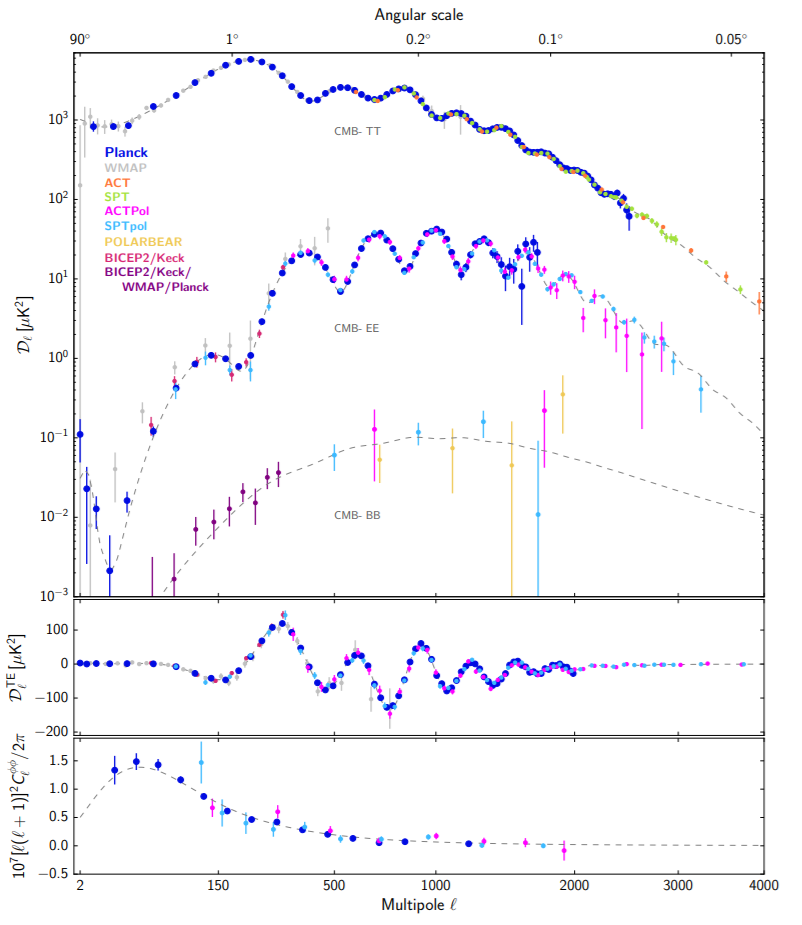
\includegraphics[width=0.9\textwidth]{cosmo_evol/CMB_compilation.png}
    \caption{Compilation of~recent CMB angular power spectrum measurements from which most cosmological inferences are drawn. The~upper panel shows the~power spectra of~the~temperature and~E-mode and~B-mode polarization signals, the~next panel the~cross-correlation spectrum between T and~E, while the~lower panel shows the~lensing deflection power spectrum. Different colours correspond to~different experiments, each retaining its original binning. For~Planck, ACTPol, and~SPTpol, the~EE points with~large error bars are not plotted (to~avoid clutter). The~dashed line shows the~best-fit \LCDM\ model to~the~Planck temperature, polarization, and~lensing data. \textit{Note:} Reprinted from \textcite{2018arXiv180706205P}.}
    \label{fig:cmb_compilation}
\end{figure}
\subsection[Supernovae]{Supernovae\footnote{\label{ftn1}Some parts of this section have already been published in \textcite{mastersthesis_vrastil}. The overtaken text is written in italics.}}
\label{ssec:supernovae}
Supernovae (SNe) are the~most straightforward tool for~studying cosmic acceleration, as they directly discovered the~acceleration in~the~first place \parencite{riess}. Type Ia supernovae (SNe Ia) are exploding stars defined by the~lack of~hydrogen and~the~presence of~silicon in~their early-time spectra \parencite{SN}, and~are a~product of~a~thermonuclear explosion of~a~C/O white dwarf. Observations show that SNe Ia have a~luminosity peak that is tightly correlated with~the~shape of~their light curves -- supernovae that rise and~fall more slowly have higher peak luminosity \parencite[first quantified by][]{SN_lum}. From observations of~(multiband) light curve shapes and~colors the~luminosity at~a~brightness peak can be predicted.

To~measure cosmic expansion with~Type Ia SNe, the~observed flux and~predicted luminosity are compared. From that the~supernova's luminosity distance can be measured. An~accurate redshift is obtained by measuring the~host galaxy (calibrator). As we can see from the~equation for~the~luminosity distance \eqref{eq:d_L}, this method gives the~distance $D_L$ in~units of~$h\mins$ Mpc. Measured relation is used to~constraint dark energy parameters.

A~recent analysis of~\textcite{Abbott_2019} uses data from the~Dark Energy Survey Supernova Program (DES-SN) -- 207 spectroscopically confirmed SNe Ia from the~first three years of~DES-SN combined with~a~low-redshift sample of~122 SNe from the~literature. For~a~flat $w$CDM\ model they found a~matter density $\Omega_m=0.321\pm0.018$ and~an~equation of~state $w=-0.978\pm0.059$, see \autoref{fig:des_sne_results}.

\begin{figure}[hbt]
    \centering
    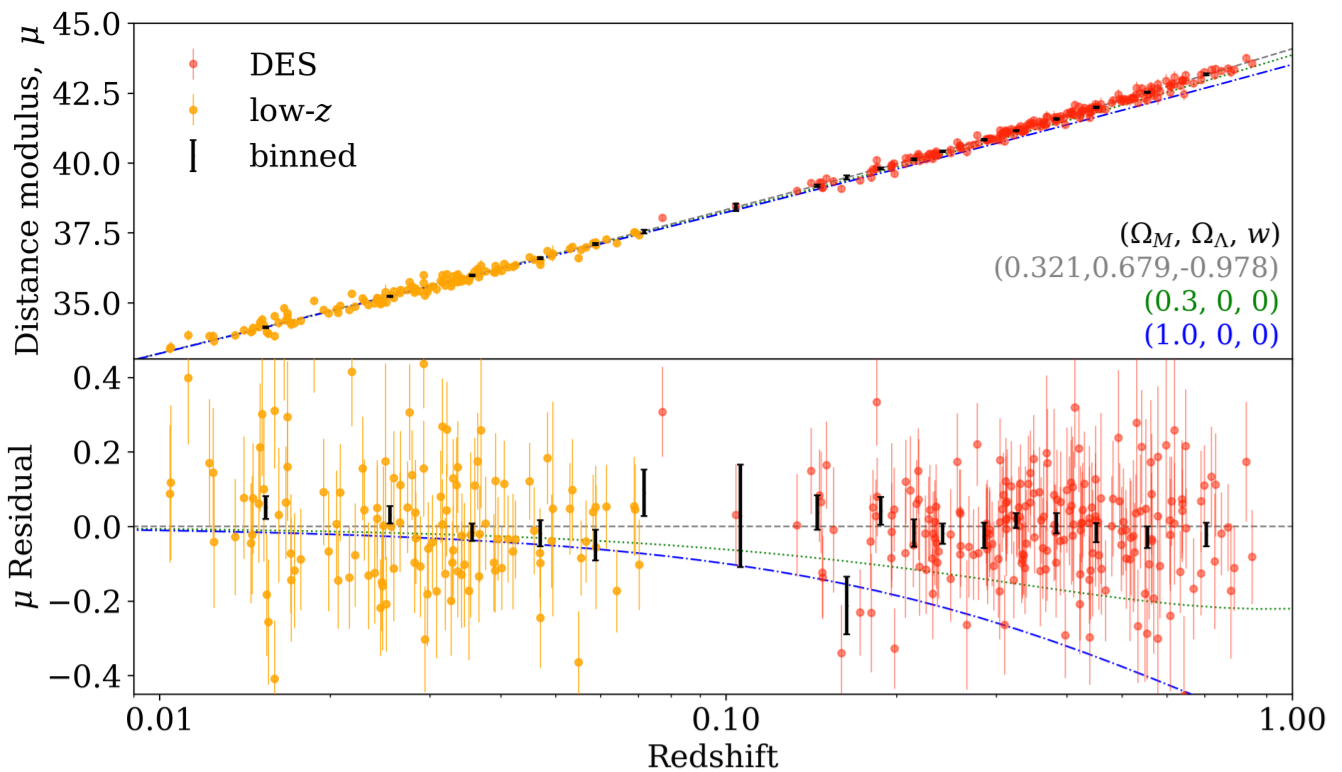
\includegraphics[width=0.7\textwidth]{cosmo_evol/DES_SNe_results.png}
    \caption{Hubble diagram for~the~DES-SN3YR sample. Top: distance modulus $(\mu =5\log [d_L/10\rm{pc}])$ from ``BEAMS with~Bias Corrections'' fit \parencite{Kessler_2017}, black bars, which are used for~cosmology fits) and~for~each SN (red, orange circles). The~dashed gray line shows best fit model, while the~green and~blue dotted lines show models with~no dark energy and~matter densities $\Omega_m = 0.3$ and~$1.0$ respectively. Bottom: residuals to~the~best fit model; $1\sigma$ error bars show 68\% confidence. \textit{Note:} Reprinted from \textcite{Abbott_2019}.}
    \label{fig:des_sne_results}
\end{figure}
\subsection[Baryonic acoustic oscillations]{Baryonic acoustic oscillations\footnoteref{ftn1}}
\label{sec:bao}
Baryonic acoustic oscillations (BAO) provide an~entirely independent way of~measuring cosmic distance. Sound waves propagating before recombination imprint a~characteristic scale on~matter clustering. The~acoustic length scale can be computed as
\eq{
r_s=\int_0^{t_\ast}{\frac{c_s(t)}{a(t)}\dd t}=\int_{z_\ast}^{\infty}{\frac{c_s(z)}{H(z)}\dd z},
}
where the~asterisk denotes time (redshift) at~recombination and~$c_s$ is the~sound speed. The~behavior of~$H(z)$ depends on~the~ratio of~the~matter density to~radiation density and~the~sound speed depends on~the~ratio of~radiation pressure to~the~energy density of~the~baryon-photon fluid, determined by the~baryon-to-photon ratio. Both the~matter-to-radiation ratio and~the~baryon-to-photon ratio can be measured from the~CMB anisotropy power spectrum. This gives $r_s\sim150$ Mpc. The~scale of~the~acoustic feature is stable to~better than 1\% accuracy, making it an~excellent standard ruler.

This effect can be detected in~the~angular clustering of~galaxies in~bins of~photometric redshift, yielding the~angular diameter distance. Furthermore, measuring the~BAO scale in~a~velocity separation allows a~direct determination of~$H(z)$. The~BAO method measures $D(z)$ in~absolute units -- Mpc not $h\mins$ Mpc like SNe measurements, and~thus BAO measurements to~the~same redshift carry different information. At~low redshift $(z\lesssim0.5)$, the~BAO method strongly complements SN measurements, while at~higher redshift $(z\gtrsim0.5)$ the~BAO method is a~powerful probe of~dark energy and~cosmic geometry.

BAO can be clearly seen in~the~correlation function \parencite[see e.g.][]{1993ApJ...412...64L} for~definition and~estimators). The~two-point correlation function $\xi(r)$ is the~excess probability $\dd P$ of~finding two pairs of~galaxies in~two volumes $\dd V_1$ and~$\dd V_2$ at~a~given comoving distance $r$
\eq{
    \label{eq:corr}
    \dd P = \bar{n}^2[1+\xi(r)]\dd V_1 \dd V_2\,,
}
where $\bar{n}$ is the~expected density of~the~distribution. The~distances are usually measured using the~redshift in~the~redshift space where the~distortions (see \autoref{sec:rsd}) cause the~redshift-space correlation $\xi(s)$ function to~vary according to~the~angle between the~separation vector and~the~line of~sight. In~\autoref{fig:xi_s} we see the~spherically averaged correlation function from \textcite{2005ApJ...633..560E} with~the~clear bump at~$100h^{-1}$ Mpc scale.
\begin{figure}[!hbt]
    \centering
    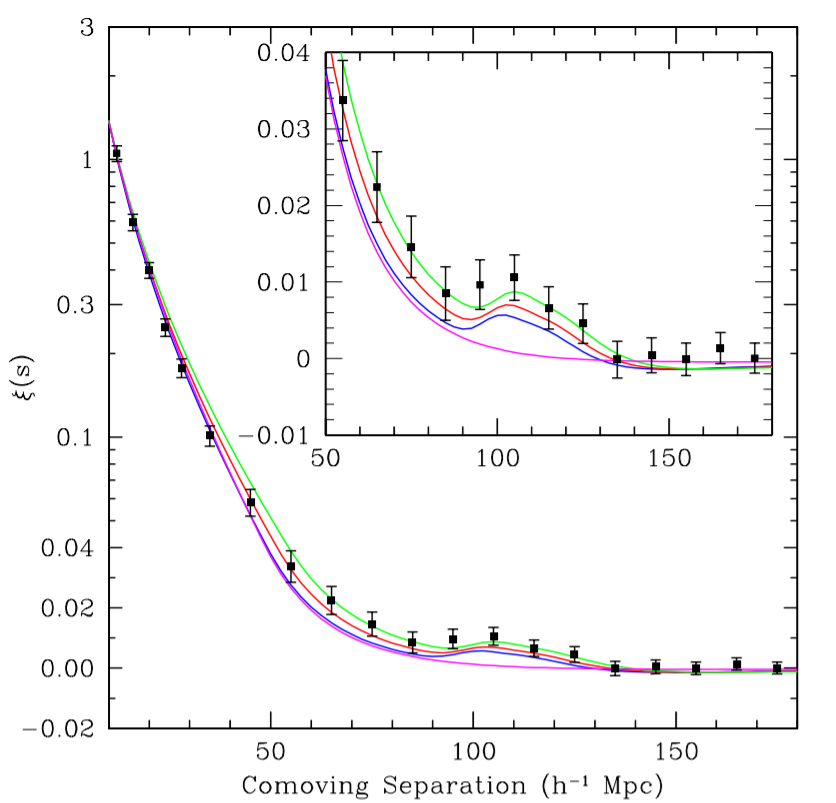
\includegraphics[width=0.7\textwidth]{cosmo_evol/bao_rsd.png}
    \caption{The~large-scale redshift-space correlation function of~the~SDSS LRG sample. The~error bars are from the~diagonal elements of~the~mock-catalog covariance matrix; however, the~points are correlated. Note that the~vertical axis mixes logarithmic and~linear scalings. The~inset shows an~expanded view with~a~linear vertical axis. The~models are $\Omega_mh^2=0.12$ (top, green), $0.13$ (red), and~$0.14$ (bottom with~peak, blue), all with~$\Omega_bh^2=0.024$ and~$n=0.89$ and~with~a~mild non-linear prescription folded in. The~magenta line shows a~pure CDM model ($\Omega_mh^2=0.105$), which lacks the~acoustic peak. It is interesting to~note that although the~data appears higher than the~models, the~covariance between the~points is soft as regards overall shifts in~$\xi(s)$. Subtracting $0.002$ from $\xi(s)$ at~all scales makes the~plot look cosmetically perfect, but changes the~best-fit $\chi^2$ by only $1.3$. The~bump at$100h^{-1}$ Mpc scale, on~the~other hand, is statistically significant. \textit{Note:} Reprinted from \textcite{2005ApJ...633..560E}.}
    \label{fig:xi_s}
\end{figure}

In~\textcite{BAO_results} present a~measurement of~the~BAO from the~three-dimensional correlation of~Lyman-$\alpha$ forest absorption and~quasars from the~SDSS Data Release 14 (the~first two years of~observations by the~eBOSS) at~redshift $z=2.35$. The~position of~the~BAO peak is used to~determine the~Hubble distance $d_H$ and~the~comoving angular diameter distance $d_A$ relative to~the~sound horizon at~the~drag epoch $r_s: d_H(z=2.35)/r_s = 9.20\pm0.36$ and~$d_M(z=2.35)/r_s = 36.3\pm1.8$. These results are $1.5\sigma$ from the~flat \LCDM\ model of~\textcite{2016A&A...594A..13P}.
\subsection[Weak lensing]{Weak lensing\footnote{Some parts of this section have already been published in \textcite{mastersthesis_vrastil}. The overtaken text is written in italics.}}
\label{ssec:wl}
Gravitational lensing is the~deflection of~light from distant sources due to~the~bending of~space-time by baryonic and~dark matter (lenses) along the~line of~sight. It is a~very useful cosmological probe because it is sensitive to~all matter regardless of~its nature. In~the~limit of~very small deflection angles, it is called weak lensing (WL). WL causes tiny distortions ($\sim0.5\%$), or ``shear'', in~galaxy sizes and~shapes. The~intrinsic size or shape of~a~given galaxy is unknown, but normally, galaxy orientations are assumed to~be random ($\sim30\%$ dispersion), so they should not exhibit statistically significant and~coherent alignments. In~the~presence of~lensing, small but coherent shears in~background galaxy images are induced. This means that WL is statistically detectable by averaging shapes over many lensed galaxies. In~principle, either the~shearing of~galaxies (shape distortion) or their magnification (size distortion) can be measured. However, in~practice, the~shape distortions are used much more widely since the~scatter in~shapes of~galaxies is less than the~scatter in~their sizes.

Weak lensing provides a~direct measure of~the~distribution of~matter, independent of~any assumptions about galaxy biasing. Since this distribution can be predicted theoretically, and~its amplitude can be directly used to~constrain cosmology, weak lensing has great potential as a~cosmological probe. The~correlation of~the~density field of~nearby galaxies with~the~lensing shear measured on~more distant galaxies is called \textit{galaxy-galaxy lensing}. Most lens systems involve sources (and~lenses) at~moderate or high redshift, and~thus can lensing probe the~geometry of~the~Universe -- the~measurement of~the~shear correlation function as a~function of~the~redshifts of~observed galaxies is called \textit{tomography}. The~scaling of~the~galaxy-galaxy lensing signal as a~function of~the~source redshift, known as \textit{cosmography}, depends purely on~geometric factors and~hence can be used to~construct a~distance-redshift relation.
\subsection[Large-scale structure]{Large-scale structure\footnote{Some parts of this section have already been published in \textcite{mastersthesis_vrastil}. The overtaken text is written in italics.}}
\label{ssec:lss}
Studying the~large-scale structures (LSS) of~the~Universe is of~great importance for~the~cosmology. Since the~clustering of~matter on~scales from galaxies to~superclusters came from quantum fluctuations in~the~very early Universe with~important modification by radiation and~baryons, the~LSS encode critical information about the~contents of~the~Universe, the~origin of~the~fluctuations, and~the~cosmic expansion background in~which the~structures evolved.

Measurements of~the~large-scale power spectrum for~the~spatial distribution of~matter as a~function of~redshift constrain the~cosmic expansion history, the~cosmological distance scale, the~growth rate of~structures, the~mass of~the~neutrinos, and~the~abundance of~dark matter. This includes the~BAO measurement of~the~distance-redshift relation (as a~standard ruler). The~BAO with~the~growth of~the~LSS in~the~Universe form two robust probes of~dark energy, and~a~potential discriminator between dark energy and~modified gravity models. Beyond the~dark energy, the~large scale power spectrum is a~probe of~both neutrino mass and~primordial non-Gaussianity.
\subsubsection{Matter power spectrum}
The~matter power spectrum $P(k)$ is defined as a~quadratic function of~the~Fourier transformation of~the~density contrast $\delta$ \parencite{2010deto.book.....A}
\eq{
  \label{eq:pk}
  P(k)(2\pi)^3\delta_{\rm D}(k-k')\equiv \left\langle \hat\delta(k)\hat\delta^*(k')\right\rangle\,,
}
where $\delta_{\rm D}$ is the~Dirac delta function and~we are averaging over possible realizations. The~power spectrum is the most used probe in cosmology in~the~linear and~mildly non-linear regime. The~power spectrum is the~Fourier transform of~the~correlation function \eqref{eq:corr}
\eq{
    \label{eq:pk_xi}
    P(k)=\int\xi(r)e^{-ik\cdot r}\dd^3r\,.
}
However, what we observe in~practice, is the~galaxy density contrast $\delta_g$, which is different from the~total matter density contrast $\delta_m$. The~two quantities are assumed to~be related by a~bias factor $b$ defined by \parencite{2010deto.book.....A}
\eq{
    b\equiv\frac{\delta_g}{\delta_m}\,,
}
from which follows $P_g(k)=b^2P_m(k)$. This simple assumption tries to incorporate non-linear physical processes, such as merging of galaxies, or evolutionary processes of stars that makes galaxies brighter or dimmer.

In~\autoref{fig:pk_planck} is shown (linear) matter power spectrum inferred from different cosmological probes \parencite{2018arXiv180706205P}.
\begin{figure}[hbt]
    \centering
    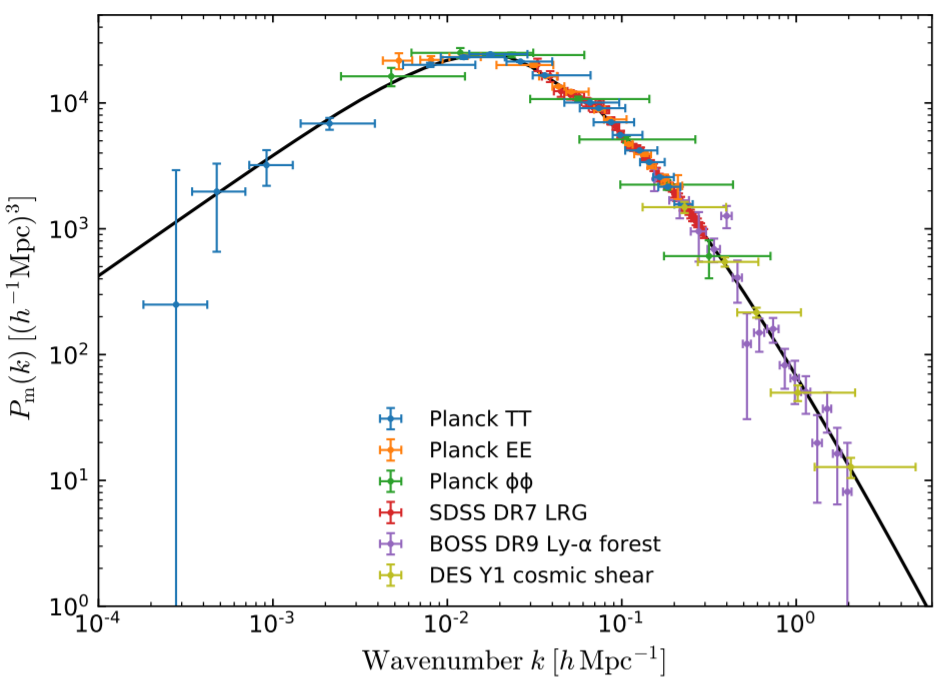
\includegraphics[width=0.7\textwidth]{cosmo_evol/pk_planck.png}
    \caption{The~(linear theory) matter power spectrum (at~z = 0) inferred from different cosmological probes. The~broad agreement of~the~model (black line) with~such a~disparate compilation of~data, spanning 14 Gyr in~time and~three decades in~scale is an~impressive testament to~the~explanatory power of~\LCDM. Earlier versions of~similar plots can be found in, for~example, \textcite{1994ARA&A..32..319W}, \textcite{1995Sci...268..829S}, \textcite{2002PhRvD..66j3508T}, and~\textcite{2004ApJ...606..702T}. A~comparison with~those papers shows that the~evolution of~the~field in~the~last two decades has been dramatic, with~\LCDM\ continuing to~provide a~good fit on~these scales. \textit{Note:} Reprinted from \textcite{2018arXiv180706205P}.}
    \label{fig:pk_planck}
\end{figure}

\subsection[Galaxy clusters]{Galaxy clusters\footnote{Some parts of this section have already been published in \textcite{mastersthesis_vrastil}. The overtaken text is written in italics.}}
\label{ssec:gc}
The~observed number density and~clustering of~galaxy clusters as a~function of~mass and~redshift provides a~powerful toolset to~constraining cosmology.  Galaxy clusters provided the~first line of~evidence for~the~existence of~dark matter \textcite{zwicky} and~cluster mass-to-light ratio measurements suggested that the~matter density in~the~universe was sub-critical \textcite{Gott}. Galaxy clusters measurements are sensitive to~both the~expansion history and~the~growth of~structure in~the~Universe enabling to~distinguish between dark energy and~modified gravity models for~cosmic acceleration. Additional probes are measurements of~the~baryonic mass fraction in~clusters, and~measurements of~the~tomographic lensing signatures through clusters.

The~basic idea of~cluster abundance studies is to~compare the~predicted space density of~massive halos to~the~observed space density of~clusters. The~basic observables are the~richness, the~number of~galaxies in~a~specified luminosity and~color range. Halo abundance is sensitive to~the~amplitude of~the~matter power spectrum $\sigma_8$ and~the~matter density $\Omega_m$, more precisely a~combination of~a~form $\sigma_8\Omega_m^q$, with~$q\approx0.4$ \textcite{white}. The~degeneracy between $\sigma_8$ and~$\Omega_m$ can be broken by measuring abundances at~a~variety of~masses.
\subsubsection{The~halo mass function}
The~halo mass function (HMF) $\dd n/\dd M$ is defined as the~number of~haloes of~mass $M$ per unit volume per unit interval in~$M$. To~describe the~halo mass function we need two other quantities, $f(\sigma)$ and~$\ln\sigma^{-1}$. The~rms linear overdensity $\sigma$ of~the~density field smoothed with~a~top-hat filter $W$ with~a~radius that encloses a~mass $M$ at~the~mean cosmic matter density is defined as \parencite{2015IJMPD..2430004B}
\eq{
    \sigma^2(M, z)=\frac{D^2(z)}{2\pi^2}\int_0^\infty{k^2P(k)W^2(k,M)\dd k}\,.
}
The~mass function is then written as
\eq{
    \label{eq:hmf}
    \dddd nM=\frac{\rho_0}{M}\dddd{\ln\sigma^{-1}}{M}f(\sigma)\,,
}
where all the~cosmological information is contained in~the~function \(f(\sigma)\) --  the~fraction of~mass in~collapsed haloes per unit interval in~$\ln\sigma$. This function depends on~how haloes are defined, usually using the~friends-of-friends (FoF) algorithm of~\textcite{1985ApJ...292..371D}. The~analytical form of~$f(\sigma)$ using the~assumption of~collisionless spherical collapse has been proposed by \textcite{1974ApJ...187..425P}
\eq{
    f_{PS}(\sigma) = \sqrt{\frac2\pi}\frac{\delta\coll}{\sigma}\exp{\left(-\frac{\delta\coll^2}{2\sigma^2}\right)}\,,
}
where the~parameter \(\delta\coll=1.686\) was introduced in~the~previous section. The~PS mass function agrees with~simulations at~$z=0$ reasonably well, but it overpredicts the~number of~low-mass halos and~underpredicts the~number of~massive halos at~the~current epoch \parencite{2007ApJ...671.1160L}. \textcite{2001MNRAS.321..372J} combined high-resolution simulations for~four different CDM cosmologies spanning a~mass range of~over 3 orders of~magnitude $(\sim10^{12}-10^{15}h^{-1}M_\odot)$, and~including several redshifts $z=0-5$. They came up with~the~following fitting function
\eq{
    \label{eq:hmf_jenkins}
    f_{Jenkins}(\sigma)=0.315\exp\left(-|\ln\sigma^{-1}+0.61|^{3.8}\right)\,.
}
As their range of~masses and~redshifts correspond to~our study case we will use this fitting formula in~our analysis (see \autoref{chpt:app_sims}).
\subsection[Strong lensing]{Strong lensing\footnote{\label{ftn2}Some parts of this section have already been published in \textcite{mastersthesis_vrastil}. The overtaken text is written in italics.}}
\label{ssec:SL}
Strong gravitational lensing (SL) refers to~the~multiple imaging of~a~background object due to~a~massive foreground object (typically clusters of~galaxies). The~resulting angular displacement, morphological distortion, and~time delay can be used to~measure dark energy parameters. Strong gravitational lensing time delays measure a~combination of~distances that combining with~other dark energy probes can further constraint cosmological parameters. The~time delays are also expected to~test gravity on~scales where the~screening mechanisms are becoming active.

Another independent way to~measure dark energy parameters with~SL is the~analysis of~systems with~multiple sets of~multiple images \textcite{SL_in_CLGs}. The~positions of~these multiple images depend strongly on~the~detailed properties of~the~lens mass distribution and~on~the~angular diameter distance ratios between the~lens, source, and~observer, they encapsulate information about the~underlying cosmology. This dependence on~the~geometry can be used to~derive constraints on~the~cosmological parameters.
\subsection[Redshift-space distortions]{Redshift-space distortions\footnoteref{ftn2}}
\label{sec:rsd}
When we observe distant galaxies, two features determine their redshifts -- the~Hubble expansion and~their peculiar velocities. The~peculiar velocities of~galaxies thus cause them to~appear displaced along the~line of~sight in~redshift space. These displacements lead to~redshift distortions in~the~pattern of~clustering of~galaxies in~redshift space and~make large scale galaxy clustering anisotropic. Redshift-space distortions (RSD) have the~tremendous advantage of~bearing information about the~dynamics of~galaxies.

The~coordinate transformation from real space $(r)$ to~redshift space $(s)$ of~a~source with~a~peculiar velocity $\bm v$ is given by \parencite{2010deto.book.....A}
\eq{
    \mb s = \mb r\left[1+\frac{u(r)-u(0)}{r}\right]\,,
}
where $u\equiv\mb v\cdot\mb r/r$. The~strength of~the~anisotropy is governed by distortion parameter $\beta = f(z)/b(z)$, where $f(z)$ is the~logarithmic growth rate of~fluctuations \eqref{eq:grw_rate} and~$b$ is the~bias. By modeling the~full redshift-space galaxy power spectrum one can obtain a~combination of~the~product of~the~matter clustering amplitude and~the~growth rate.

Anisotropy of~galaxy clustering offers an~alternative to~weak lensing and~cluster abundances as a~tool for~measuring the~growth of~structures. RSD directly measures the~rate at~which structure is growing at~the~redshift of~observation, unlike WL and~galaxy cluster measurements which measure the~rate of~growth at~multiple redshifts. RSD measurements can improve constraints on~dark energy models and~they can be used to~constrain departures from GR by testing the~consistency of~the~growth and~expansion histories. The~key challenge in~modeling RSD is accounting for~non-linear effects, including non-linear or scale-dependent bias between galaxies and~matter, at~the~level of~accuracy demanded by the~LSST's precision. 
\section{Cosmological Surveys}
There are many projects and~missions which study properties of~the~dark energy, either as a~main scientific goal or as a~complementary program. Here we mention some of the biggest surveys while directing the reader for further references.
\subsection{Sloan Digital Sky Surveys}
Sloan Digital Sky Surveys (SDSS, \cite{SDSS}) aims to~create the~most detailed three-dimensional maps of~the~Universe. From the~beginning of~regular surveys in~2000 till 2014 there were seven finished surveys in~total (SDSS-I/II results \cite{SDSS_I_II}, SDSS-III results \cite{BOSS_results}), while there are three ongoing surveys from 2014 (SDSS-IV, \cite{2017AJ....154...28B}) and~a~planned panoptic spectroscopic survey (SDSS-V, \cite{2017arXiv171103234K}) which will start collecting data in~summer 2020. The~Baryon Oscillation Spectroscopic Survey (BOSS, \cite{BOSS}) was a~six-year program (Fall 2009 -- Spring 2014) designed to~measure the~scale of~baryonic acoustic oscillations (BAO, see \autoref{sec:bao}) in~the~clustering of~matter. The~Extended Baryon Oscillation Spectroscopic Survey (eBOSS, \cite{2016AJ....151...44D}) is the~new cosmological survey within a~SDSS-IV six-year program. eBOSS conducts observations of~galaxies and quasars and will expand the~selection of~luminous red galaxies beyond that probed by BOSS.
\subsection{Dark Energy Survey}
The~Dark Energy Survey (DES) is a program designed to~uncover the~nature of~dark energy by measuring the history of~cosmic expansion with~high precision. DES is an~optical near-infrared survey of~5000 deg\sq\ of~the~South Galactic Cap. Starting in~August of~2013 and~continuing till January 2019, DES begun to~survey a~large swath of~the~southern sky out to~vast distances in~order to~provide new clues to~these most fundamental questions \parencite{DES}.
\subsection{Euclid}
Euclid is an~ESA (European Space Agency) high-precision space mission designed to study dark matter and dark energy through mapping the~geometry and~evolution of~the~Universe \parencite{euclid,2010arXiv1001.0061R}. For this purpose, the~Euclid will mainly use two independent cosmological probes -- weak gravitational lensing and~baryonic acoustic oscillation -- out to~redshift $z\sim2$. As complementary probes, Euclid will use galaxy clusters and~the~Integrated Sachs--Wolfe effect. The Euclid mission will start in~mid-2022. The~overview of~the~Euclid system design and~scientific requirements can be found in~\cite{2011arXiv1110.3193L}.
\subsection{Vera C. Rubin Observatory}
The~Vera C. Rubin Observatory project, previously known as the~Large Synoptic Survey Telescope, will conduct the~10-year Legacy Survey of~Space and~Time (LSST, \cite{lsst}). LSST is a~ground-based telescope in Chile and will produce a~6-band (300 -- 1100 nm) wide-field deep astronomical survey over 20,000 deg\sq\ of~the~southern sky. The LSST will scan the sky very rapidly (more than 800 images each night) and each patch of~the~sky will be visited about 1000 times during the whole survey. LSST`s data will be used for studying the dark matter and~the~dark energy. LSST will also detect and~track potentially hazardous asteroids. The~project is in~the~construction phase and~will begin its full science operations in~2022 \parencite{lsst_web}.
\subsection{Planck}
The~Planck mission (\cite{planck}) was a~European Space Agency mission with~significant participation from NASA. It was launched into space on~May 14, 2009, and~was orbiting the~second Lagrange point of~our Earth-sun system, about 1.5 million km (930,000 miles) away. Planck was measuring the~Cosmic Microwave Background (CMB) over a~broad range of~far-infrared wavelengths. The mission`s goal was to study the~geometry and~contents of~the~Universe \parencite[for results, see][]{planck_cosm}. Planck`s mission ended on~23 October 2013, after nearly 4.5 years of operations \parencite{planck_web}.
\subsection{Nancy Grace Roman Space Telescope}
The~Nancy Grace Roman Space Telescope (formerly known as WFIRST, the~Wide Field Infrared Survey Telescope) is a~NASA space mission designed to~study dark energy, exoplanets, and~infrared astrophysics \parencite{wmap_web}. It will perform wide-field imaging and spectroscopic survey of~the~near-infrared sky. These data will be used to determine the~expansion history of~the~Universe and~the~growth history of~larges-scale structures. WFIRST`s mission should start in~the~mid-2020s \parencite{WFIRST_report}.
 \clearpage{}
\clearpage{}\chapter{Dark Energy and~Modified Gravity}
\label{chpt:de_mg}
In~this chapter we briefly introduce how we can modify Einstein's general relativity, what are reasons for~such modifications (the~cosmological constant problem), and~the~main ideas behind adding new degrees of~freedom to~the~Einstein equations. We describe one particular model of~modified gravity in~more detail -- the~$f(R)$ theory and~chameleon gravity. We will study the~behavior of~the~chameleon field in~spherical systems using numerical techniques.

Some review parts of this chapter has already been studied and described in author`s work \textcite{mastersthesis_vrastil}. In this work, we deal with the~same topic of the $f(R)$ gravity. We also use various notations and equations we already defined in~the~former work and we need them here, such as the~chameleon field $\chi$ and related equations. As we further develop the original study of the chameleon, we also took over some parts of the text. We use the text in sections \hyperref[sec:fR]{\fR\ gravity}, \hyperref[sec_cham]{Chameleon Gravity}, and \hyperref[sec:other]{Other theories}, where a general overview of~other~interesting theories is presented. In section \hyperref[sec_cham]{Chameleon Gravity} we also extended our previous analysis of chameleon field on cosmological scales and we also extended the study of the chameleon in spherical systems on the scales of galaxy clusters.

\section{Standard $\Lambda$CDM model -- successes and~issues}
The~standard cosmological model, the~\LCDM\ model or the~concordance model, assumes that the~Universe originated in~the~Big Bang from infinitely hot and dense energy, and~now is the~Universe composed of~about 5\% ordinary matter, 27\% dark matter, and~68\% dark energy \parencite{redefineLCDM}. The~\LCDM\ model depends on two theoretical models -- the~Standard Model of~Particle Physics and~ the~General Theory of~Relativity. The~model also assumes that the~universe is homogeneous and~isotropic on~sufficiently large (cosmic) scales. The~model is mathematically described above in~\autoref{chpt:cosmo_evol}.

The~\LCDM\ model represents the Universe with~a~cosmological constant \(\Lambda\) described by general relativity. This cosmological constant is now associated with~dark energy. The other requirement of this model is the presence of sufficiently massive dark matter particles -- the cold dark matter. However, the~nature of~both dark energy and~dark matter is unknown.

In~1948, \textcite{PhysRev.74.505.2} suggested that the~elements could have been made during the~early hot matter-energy phase associated with~the~Big Bang and~predicted their representation -- hydrogen about 75\%, helium about 25\%, and~small amounts of~deuterium, lithium, and~other light elements.

The~other success of~the~Big bang model is the~prediction of~the~Cosmic Microwave Background (CMB) radiation and~its temperature. \textcite{1948Natur.162..774A} predicted the~temperature of~the~CMB to~be approximately 5 K, very close to~the~current value of~2.73 K, determined by the~COBE satellite. Besides, the~COBE results showed that the CMB is extremely isotropic and homogeneous. These smooth properties of the CMB are not easily explainable in the original Big Bang model and they have led to the~theory of~inflation \parencite{1981PhRvD..23..347G}. This model predicts strongly accelerated expansion of the Universe during its very early stage.

The~\LCDM\ model has an~additional major assumption about the~existence of~dark matter. The original need of~dark matter came from observations of galaxy clusters \parencite{zwicky} and, later, from observations of~galaxy rotation curves \parencite{1980ApJ...238..471R} and 21 cm rotation curves for~neutral hydrogen gas \parencite{1978PhDT.......195B}. All these objects moved under gravitational forces that could not be caused only by the~visible matter. Considerably more gravitational mass was needed to explain these anomalous movements. This missing matter was called dark matter. Up-to-date, no experiment searching for direct evidence of the dark matter has confirmed its existence and its nature remains unexplained.

Two sets of~observations of~supernovae of~Type Ia by \textcite{riess} and~\textcite{1999ApJ...517..565P} suggested that the~expansion of~the~universe is accelerating. As standard forms of matter cause only attractive gravitational forces, which decelerate the expansion, some new kind of matter-energy is needed to overcome the gravity. This mysterious energy was named dark energy.

\subsection{Cosmological constant problem}
\label{ssec:lambda}
The~standard cosmological \LCDM\ model described above is in~a~good agreement with~all measurements of~CMB \parencite{planck_cosm}, type Ia supernovae \parencite{Abbott_2019}, or BAO \parencite{BAO_results}. However, this concordance model, and~namely the~cosmological constant, has some significant fundamental problems. Usually, the~fine-tuning of~the~cosmological constant is presented as the~main issue but the~real issue with~the~cosmological constant is radiative instability, and~the~need to~\textbf{repeatedly} fine-tune whenever the~higher loop corrections are included. We will describe here only the~main idea behind these problems, for~a~more detailed overview see e.g. \textcite{2015arXiv150205296P,2012CRPhy..13..566M}.

The~action of~the~general relativity, together with~the~action describing matter, is
\eq{
	\label{eq:S_GR}
	S=\frac{\Mpl^2}{2}\int\dd^4x\dg\left(R-2\Lambda_B\right)+S_m[\psi_m;g_\uv]\,,
}
where $\Mpl\equiv(\sqrt{8\pi G})^{-1}$ is the~reduced Planck mass, $R$ is the~Ricci scalar (curvature), $\Lambda_B$ the~bare cosmological constant and~$S_m[\psi_m;g_\uv]$ represents the~action of~matter fields. The~first term $(R)$ is the~standard Einstein-Hilbert action. The~second term consists of the~\textit{bare} cosmological constant and~it is just a~new parameter of~the~total action. The cosmology constant in the action above is compatible with~the~principle of~general covariance and it is natural from the~relativistic point of view. The~third term in~the~action denotes the~generic matter action. Variation of~the~action \eqref{eq:S_GR} with~respect to~the~metric tensor $g\uv$ leads to~the~Einstein equations
\eq{
    R_\uv-\frac12Rg_\uv+\Lambda_Bg_\uv=\frac{1}{\Mpl^2}T_\uv\,,
}
where the~stress-energy tensor is defined by
\eq{
    T_\uv=-\frac{2}{\dg}\frac{\delta S_m}{\delta g^\uv}\,.
}
As shown by \textcite{1968SPhD...12.1040S}, the quantum field theory changes the~situation. The~stress-energy tensor of~a~field placed in~the~vacuum is given by
\eq{
    \left\langle0\left|T_\uv\right|0\right\rangle=-\rho\vac g_\uv\,,
}
where $\rho\vac$ is the~constant energy density of~the~vacuum. The~vacuum fluctuations are, therefore, just another form of~energy and as such, they must gravitate. If we take them into account,  the~Einstein equations read
\eq{
    R_\uv-\frac12Rg_\uv+\Lambda\eff g_\uv=\frac{1}{\Mpl^2}T_\uv\,,
}
where
\eq{
    \Lambda\eff=\Lambda_B+\frac{1}{\Mpl^2}\rho\vac\,.
}
The~effective cosmological constant $\Lambda\eff$ is the~sum of the~bare cosmological constant and~a~contribution from the~vacuum fluctuations. When making observations using the~Einstein equations, it is this effective cosmological constant that governs the results. Another~problem is that $\rho\vac$ includes several different terms, each of them huge in~comparison with~the~observed value of~$\Lambda\eff$ and~need to~be fine-tuned.
\subsubsection{Phase Transitions}
\begin{sloppypar}
Another problem with~fine-tuning of~the~cosmological constant comes from changes in~the~vacuum energy during phase transitions such as was the~electroweak phase transition. The~contribution to~the~vacuum energy coming from the~minimum of~a~potential of~some field, in~this case, the~Higgs field, changes as the~field takes its new position after the~transition. One can calculate this contribution \parencite{2012CRPhy..13..566M} and~for~the~mass of~the~Higgs boson $m_H=125$ GeV arrives at
\end{sloppypar}
\eq{
    \rho\vac^{EW}\simeq -10^{55}\rho\crit\,.
}
For~the~quantum chromodynamics transition, one can compute
\eq{
    \rho\vac^{EW}\simeq10^{45}\rho\crit\,.
}
If we fine-tune the~vacuum energy to~be zero today it had to~be non-zero (and~huge) before each of~these transitions.
\subsubsection{Zero-Point Energy Density}
When we consider a~simple real free scalar field with~the~potential $V(\Phi)=2m^2\Phi^2/2)$ we will arrive at~the~vacuum energy
\eq{
    \left\langle \rho \right\rangle = \left\langle0\left|T_{00}\right|0\right\rangle=\frac{1}{2\pi^3}\frac12\int\dd^3k\sqrt{k^2+m^2}\,.
}
This contribution to~the~cosmological constant blows up in~the~ultra-violet regime and~is infinite. But this is nothing new in~the~quantum field theory. If we apply the~dimensional regularization \parencite{tHooft:1972tcz} and~subtract the~pole, as usual, one is left with~a~finite energy density of~the~vacuum
\eq{
    \left\langle \rho \right\rangle = \frac{m^4}{64\pi^2}\ln{\left(\frac{m^2}{\mu^2}\right)}\,,
}
where $\mu$ is a~regularization scale. We see that the~contribution is proportional to~the~fourth power of~the~mass of~the~particle and~therefore, e.g., the~photon does not contribute to~the~vacuum energy density. The~equation was derived for~the~free scalar field but similar contributions with~different pre-factors can be computed for~all other fields. The~overall vacuum energy density is then
\eq{
    \label{eq:vac_all}
    \rho\vac=\sum_in_i\frac{m_i^4}{64\pi^4}\ln{\left(\frac{m_i^2}{\mu^2}\right)} + \rho_B + \rho\vac^{EW} + \rho\vac^{QCD}\,,
}
where $n_H=1$ stands for~the~Higgs boson, $n_f=4$ for~fermions and~$n_V=3$ for~massive vector fields. For~the~renormalization scale $\mu\simeq3\times10^{-25}$, as discussed in~\textcite{2011arXiv1105.6296K}, one calculates the~contribution from the~zero-point energy of~particles to~be  $\rho\vac\simeq-2\times10^8$ GeV$^4$
\subsubsection{Radiative instability}
The~one-loop contributions \eqref{eq:vac_all} to~the~vacuum energy can be fine-tuned via the~bare cosmological constant and~associated $\rho_B$. Even though the~cancellation has to~be very precise (one part in~$\sim10^{60}$) we can be fine with~this solution. Problems come with~two-loops correction which is not significantly suppressed with~respect to~the~one-loop contribution \parencite{2012CRPhy..13..566M}. The~cancellation imposed at~one-loop is spoilt and~one must retune the~finite contributions in~the~counterterm to~similar degree of~accuracy. If we go further, to~the~three loops, four loops, and~so on, we are required to~fine-tune each time to~extreme accuracy. This is radiative instability and~the~main cosmological constant problem.

As we know that vacuum energy really does exist, as evidenced by the~Lamb shift \parencite{2020Physi...2..105M} or the~Casimir effect \parencite{2006BrJPh..36.1137F}, and~that this energy does gravitate, as indicated by measurements of~the~ratio of~gravitational mass to~inertial mass for~heavy nuclei \parencite{Braginskii:1971tn}, we should take the~radiative instability as a~serious problem regarding the~cosmological constant and~be willing to~look for~alternatives. Other reasons for~studying the~modifications of~gravity may include the~following \parencite{2006hep.th....1213N}. Modified gravity:
\begin{itemize}
	\item can provide natural unification of~the~early-time inflation and~late-time acceleration
	\item can serve as the~basis for~a~unified explanation of~dark energy and~dark matter
	\item is expected to~be useful in~high energy physics (e.g. for~the~explanation of~hierarchy problem or unification of~GUTs with~gravity)
\end{itemize} 
\section[$f(R)$-gravity]{$f(R)$-gravity\footnote{Some parts of this section have already been published in \textcite{mastersthesis_vrastil}. The overtaken text is written in italics.}}
\label{sec:fR}
One of~the~simplest modified gravity models is the~so-called $f(R)$ gravity in~which we consider general functions of~the~Ricci scalar $R$ in~the~action
\eq{
	\label{eq:S_fr}
	S=\frac{\Mpl^2}{2}\int\dd^4x\dg\left[F(R)\right]+S_m[\psi_m;g_\uv]\,,
}
where $F(R)=R+f(R)$ and~$S_m$ is the~matter action with~matter fields $\psi_m$ which are minimally coupled to~gravity, i.e. they interact with~gravity only through the~determinant of~the~metric $\dg$ and~the~canonical kinetic term $-\frac12g^\uv\partial_\mu\psi\partial_\nu\psi$. The~matter fields $\psi_m$ obey standard conservation equations and~therefore the~metric $g_\uv$ corresponds to~the~Jordan frame.

Variation with~respect to~the~metric $g^\uv$ gives us the~equation of~motion
\eq{
	\label{eq:fR}
	F\R R_\uv-\frac{1}{2}F g_\uv+g_\uv\Box F\R-\nabla_\mu\nabla_\nu F\R=\frac{1}{\Mpl^2}T_\uv\,.
}
For~$f(R)=-2\Lambda$ the~standard Einstein gravity is reconstructed. Taking the~trace of~\eqref{eq:fR} we get
\eq{
	\label{eq:fR_tr}
	3\Box F\R+F\R R-2F=\frac{1}{\Mpl^2}T\,.
}
We see that there is a~propagating scalar degree of~freedom, so-called \textit{scalaron} $F\R$ with~mass $m^2=F\R/(3F\RR)$, which corresponds to~the~scalar field conformally coupled to~matter in~the~Einstein frame.

To~get the~inflation we need a~solution that approaches the~de Sitter solution characterized by vacuum space with~constant positive curvature. Thus $\Box F\R=0$ and~\eqref{eq:fR_tr} becomes
\eq{
	F\R R-2F=0.
}
For~example, the~model $F(R)=\alpha R^2$ gives rise to~an~asymptotically exact de Sitter solution and~can be responsible for~the~inflation in~the~early Universe. In~the~model $f(R) = R + \alpha R^2$, the~inflation ends when the~quadratic term becomes smaller than the~linear term. As at~the~present epoch is the~curvature very small this model is not suitable to~realize the~present cosmic acceleration. Models like $f(R)=-\alpha/R^n$ with~$\alpha>0,\ n>0$ could in~principle give rise to~the~present acceleration. However, these models do not satisfy local gravity constraints because of~the~instability associated with~negative values of~$f\RR$. Moreover, the~standard matter epoch is not present because of~a~large coupling between the~Ricci scalar and~the~non-relativistic matter.

There are four conditions for~the~viability of~\fR\ models \parencite{Amendola_2007}
\begin{itemize}
	\item $F\R>0\ (\rm{for\ } R>R_0)$, where $R_0$ is the~Ricci scalar at~the~present epoch,\\
	-- required to~avoid anti-gravity \parencite{2010deto.book.....A}\\
	\item $F\RR>0\ (\rm{for\ } R>R_0)$,\\
	-- required for~consistency with~local gravity tests \parencite{2005gr.qc.....5136O}, for the~presence of~the~matter-dominated epoch \parencite{2007PhRvL..98m1302A} and~the~stability of~cosmological perturbations \parencite{2007PhRvD..75d4004S}\\
	\item $F(R)\rightarrow R-2\Lambda\ (\rm{for\ } R\gg R_0)$,\\
	-- required for~consistency with~local gravity tests \parencite{2008PhRvD..77b3507T} and~for the~presence of~the~matter-dominated epoch \parencite{Amendola_2007}\\
	\item $0<\frac{RF\RR}{F\R}<1\ (\rm{for\ } F\R R-2F=0)$.\\
	-- required for~the~stability of~the~late-time de Sitter solution \parencite{1988PhLB..202..198M}
\end{itemize}
Some examples of~\fR\ models that satisfy these conditions:
\eq{
	f(R)&=-\mu R_c(R/R_c)^p	&\mbox{for\ }&0<p<1;\ \mu,R_c>0\,,\\
	f(R)&=-\mu R_c\frac{(R/R_c)^{2n}}{(R/R_c)^{2n}+1} 	&\mbox{for\ }&n,\mu,R_c>0\,,\\
	f(R)&=-\mu R_c\left[1-(1+R^2/R^2_c)^{-n}\right] 	&\mbox{for\ }&n,\mu,R_c>0\,,\\
	f(R)&=-\mu R_c\tanh(R/R_c)	&\mbox{for\ }&\mu,R_c>0\,.
}
One of~the~main predictions of~\fR\ gravity is a~different structure formation history than in~\LCDM. For~the~large-scale structure formation on~subhorizon scales \mbox{$k\gg H$} in~quasi-static approximation one gets the~modified equation for~matter density perturbation \parencite{2011RSPTA.369.4947B}
\eq{
	\ddot{\delta}_m+2H\dot{\delta}_m-4\pi G\eff \rho_m\delta_m\approx0\,,
}
where the~effective gravitational constant is defined by
\eq{
	G\eff \equiv\frac{G}{1+f\R}\frac{4k^2+3a^2m^2}{3k^2+3a^2m^2}\,.
}
On~scales much larger than the~scalaron Compton wavelength $m\mins$, gravity is unmodified aside from the~overall reduction factor $f\R$. However, on~smaller scales the~gravitational coupling increases by the~factor $4/3$. As the~scalaron mass $m$ and~the~factor $f\R$ depend on~curvature (local density), the~chameleon mechanism discussed earlier can prevent the~detection of~this effect in~the~Solar System.

\subsection{Jordan vs. Einstein Frame}
The~action \eqref{eq:S_fr} is described in~the~so-called Jordan frame, where the~matter fields are minimally coupled to~the~metric and~follow geodesics. We can also describe the~action in~the~so-called Einstein frame, where ``standard'' gravity is restored. Using the~conformal transformations
\eq{
\label{eins_trans}
\begin{split}
\tilde{g}_\uv &\equiv F\R g_\uv \,, \\
\phi &\equiv\Mpl\sqrt\frac32\ln F\R \,, \\
A(\phi) &\equiv F\R^{-1/2}\,, \\
V(\phi) &\equiv\frac{\Mpl^2}{2} \frac{F\R R - F}{F\R^2}\,,
\end{split}
}
we can rewrite the~action \eqref{eq:S_fr}
\eq{
\label{eq:S_ein_fr}
S=\int\dd^4x\dgt\left[\frac{\Mpl^2}{2}\tilde{R} - \frac12(\partial\phi)^2-V(\phi)\right]+S_m[\psi_m;A^2(\phi)\tilde{g}_\uv],
}
where tildes denote quantities in~the~Einstein frame. This action looks like the~Einstein-Hilbert action with~minimally coupled scalar but now the~matter fields are also coupled with~the~scalar field via factor $A(\phi)$. 

There is a~difference between whether one takes action \eqref{eq:S_fr} or \eqref{eq:S_ein_fr} to~be the~fundamental action defining the~modified gravity. In~the~former one, there is only one coupling constant $\beta$, defined by $A(\phi)=\exp(\beta\phi/\Mpl)$, for~all matter fields. If one takes the~action in~the~Einstein frame to~be the~fundamental one the~matter action is replaced by $S_m[\psi_m;A^2(\phi)\tilde{g}_\uv]\rightarrow S_i[\psi_i;A_i^2(\phi)\tilde{g}_\uv]$ where one can define the~coupling strengths $\beta_i$ to~the~different matter components to~be different. This is very important for~tests of~modified gravity. For~instance, if there is minimal coupling to~the~baryonic matter, $\beta_b=0$, Solar System or astrophysical tests do not constraint coupling strength to~the~cold matter $\beta_c$ whereas the~cosmological observations do.

Note that the~coupling constant for~\fR\ is $\beta=\sqrt{1/6}$ but for~other more general theories this coupling can vary. Even for~\fR\ theories, one expects that loop corrections can change the~coupling strength. Also, other theories such as the~Jordan--Brans--Dicke theory, Kaluza--Klein theories, and~higher derivative theories of~gravity, can be formulated in~two different ways \parencite{Faraoni:1998qx}.

These two conformally related frames are physically equivalent, i.e. physical observations are frame independent, but the~frame dependence of~cosmological perturbations has led to~confusion in~the~past. There have been many debates about the~(in)equivalence of~these frames \parencite{Postma:2014vaa} and~whether which one is the~physical \parencite{Faraoni:1999hp}. Many contradictory arguments (sometimes incorrect) of~both sides result in~confusion and~ambiguous viewpoints.

It has been shown in~\textcite{Magnano:1993bd} that these two frames are \textit{mathematically} equivalent, i.e. every solution in~one frame implies an~existence of~a~solution in~the~other frame and~can be mapped into this frame. The~confusion about their physical equivalence comes from interpretations of~experiment results. For~example, \textit{ordinary} cosmology described by Einstein’s theory leads to~an~expanding universe solution. Coming to~the~Jordan frame we can interpret the~scale factor as a~scalar field which is coupled to~matter. In~this case, the~redshift of~spectral lines is no longer interpreted as an~effect due to~the~expansion of~the~Universe, but due to~growth of~coupling constants such that the~present transition energies are higher than those in~the~past. Hence the~Jordan frame physicist does not see an~expanding Universe, but growing coupling constants. Nevertheless, the~measured redshift of~spectral lines is the~same for~both frames.

Both frames have some issues with~fundamental principles. In~the~Jordan frame, the~weak energy condition can be violated and~hence states with~the~negative energy are possible. Moreover, there is no guarantee of~stability of~the~ground state. All \textit{classical} fields are believed to~satisfy the~energy condition but no so in~quantum theories. On~the~other hand in~the~Einstein frame, the~weak energy condition is satisfied but due to~the~non-universal coupling of~the~matter fields, the~equivalence principle is violated. However, this violation is only weak and~can pass the~Solar system tests.

\subsection{Screening Mechanisms}
We know that general relativity with~the~cosmological constant and~assumptions about the~cold dark matter can describe our universe very well. That means that any modified cosmology must be able to~recover \LCDM\ cosmology to~high accuracy. This is not normally an~issue. However, since modifications of~GR typically involve an~extra scalar degree of~freedom there are interactions with~matter that are unavoidable -- no symmetry can prevent all couplings to~the~standard model. This coupling to~matter means that there should be a~fifth force. Because we do not see any fifth forces or modifications of~gravity in~the~laboratory or in~the~Solar System we need to~suppress these fifth forces -- we need some sort of~a~\textit{screening mechanism}.

The~nature of~the~screening mechanisms can be different. Let us start from \eqref{eq:S_ein_fr} with~the~generalized kinetic term $-\frac12 Z(\phi,\partial\phi,...)(\partial\phi)^2$. We can solve the~equations of~motion for~the~background in~a~minimum of~a~potential $V(\phi)$ and~write $\phi=\phi_0+\delta\phi$, where $\phi_0$ is a~background solution and~$\delta\phi$ is a~fluctuation. The~Lagrangian density for~the~fluctuations to~the~second order (first order vanishes) is
\eq{
\LL\propto-\frac12 Z(\phi_0)(\partial\delta\phi)^2+\frac12 m^2(\phi_0)\delta\phi^2+\frac{\beta(\phi_0)}{M_p}\delta\phi\delta T,
}
where $m^2(\phi)\equiv V_{,\phi\phi}(\phi)$. Now, any of~these three terms can serve as a~screening term:
\begin{itemize}
	\item  \textit{Large inertia} -- a~large $Z$ makes it hard for~the~scalar to~propagate and~leads to~the~kinetic type of~the~screening, where first or second derivatives being important; e.g. Galileons \parencite{2009PhRvD..79f4036N}, massive gravity \parencite{2012RvMP...84..671H} or Vainshtein mechanism \parencite{2013CQGra..30r4001B};
	\item \textit{Large mass} --  a~large $m$ means the~scalar propagates only over short distances and~leads to~the~chameleon type of~the~screening, where in~regions of~high-density, such as on~the~Earth, the~field acquires a~large mass -- the~Chameleon mechanism \parencite{Waterhouse:2006wv};
	\item \textit{Weak coupling} -- a~small $\beta$ in~regions of~high density makes the~interaction with~matter fields weaker and~leads to~symmetron \parencite{2010PhRvL.104w1301H}) or varying dilaton \parencite{Damour:1994zq,2011PhRvD..83j4026B} theories.
\end{itemize} 
\section[Chameleon Gravity]{Chameleon Gravity\footnote{Some parts of this section have already been published in \textcite{mastersthesis_vrastil}. The overtaken text is written in italics.}}
\label{sec_cham}
We now describe \fR\ gravities exhibiting the~chameleon mechanism in~more detail. As stated, this mechanism uses the~large mass of~the~chameleon field in~high-density regions and~chameleon gravity can satisfy tests of~the~equivalence principle in~the~Solar System. The~action of~a~chameleon scalar field $\chi$ in~the~Einstein frame is given by the~action \eqref{eq:S_ein_fr}. Varying the~action with~respect to~the~field $\chi$ one can obtain the~equation of~motion
\eq{
	\label{eom:cham}
	\Box\chi=V_{,\chi}-\sum_i\frac{\beta_i}{\Mpl}e^{4\beta_i\chi/\Mpl}g^\uv_{(i)}T^{(i)}_\uv,
}
where $T^{(i)}_\uv$ is the~stress-energy tensor for~the~$i$-th matter component. For~a~perfect isotropic fluid the~equation of~motion is
\eq{
	\Box\chi=V_{,\chi}+\sum_i(1-3w_i)\frac{\beta_i}{\Mpl}\rho_i e^{(1-3w_i)\beta_i\chi/\Mpl}.
}
This equation could be read as
\eq{
	\Box\chi=V_{\eff,\chi}\left(\chi\right),
}
where the~effective potential $V_{\eff}$ is defined by
\eq{
	V_{\eff}\left(\chi\right)\equiv V(\chi)+\sum_i\rho_i e^{(1-3w_i)\beta_i\chi/\Mpl}.
}
If the~couplings $\beta_i$ are the~same for~each matter component with~the~same $w$ (we can omit the~radiation in~the~sum) and~the~overall density is $\rho=\sum_i\rho_i$, then the~effective potential reads
\eq{
	V_{\eff}\left(\chi\right)\equiv V(\chi)+\rho e^{(1-3w)\beta\chi/\Mpl}.
}
For~the~quasi-static and~weak $(\beta\chi/\Mpl\ll1)$ field in~a~weak gravity background (the~Minkowski background) with~the~non-relativistic matter, the~equation further simplifies as
\eq{
	\label{eq:cham}
	\Delta \chi=\frac{\beta}{\Mpl}\rho+V_{,\chi},
}
which looks like the~normal Poisson equation but with~an~extra non-linear term.
\subsection{Chameleon Force}
The~interaction of~the~chameleon field with~matter is described by the~conformal coupling \eqref{eins_trans}. Free matter fields $\psi_m^{(i)}$ follow geodesics of~the~Jordan frame metric. In~the~Einstein frame, they follow modified trajectories affected by the~chameleon field \parencite{Waterhouse:2006wv}
\eq{
\frac{\dd^2x^\mu}{\dd\tau^2}+\Gamma^\mu_{\alpha\beta}\dddd{x^\alpha}{\tau}\dddd{x^\beta}{\tau}=-\frac{\beta_i}{\Mpl}\left(2\chi_{,\alpha}\dddd{x^\alpha}{\tau}\dddd{x^\mu}{\tau}+g^{\beta\mu}\chi_{,\beta}\right).
}
Note that the~chameleon force violates the~weak Equivalence Principle only if there exist two matter species with~differing values of~$\beta_i$. In~the~non-relativistic limit, a~test particle of~mass $m$ of~species $i$ in~a~static chameleon field $\chi$ is moving under a~force $\mb{F}_\chi$ given by
\eq{
\label{cham_force}
\frac{\mb{F}_\chi}{m}=-\frac{\beta_i}{\Mpl}\mb{\nabla}\chi
}
\subsection{Chameleon mechanism}
As discussed previously, we need some sort of~a~screening mechanism to~avoid Solar System tests of~GR. It means as seen from \eqref{cham_force} that the~chameleon potential needs to~approach some constant value in~dense regions or at~least have a~marginally suppressed amplitude.

Suppose we have a~background solution $\chi_0$ which minimizes the~effective potential with~$\rho=\rho_0$. For~small fluctuations $\chi=\chi_0+\delta\chi$ and~$\rho=\rho_0+\delta\rho$ we can linearize \eqref{eq:cham} to~obtain
\eq{
\label{eq:cham_lin}
\Delta \delta\chi=\frac{\beta}{\Mpl}\delta\rho+m^2_0\delta\chi,
}
where
\eq{
m^2_0\equiv V_{,\chi\chi}(\chi_0).
}
Except for~the~screening term, the~equation \eqref{eq:cham_lin} has the~same behavior as the~Poisson equation for~the~Newtonian potential $\Phi_G$. For~a~spherically symmetric density profile, this gives solution
\eq{
\chi=\chi_0+2\beta\Mpl\Phi_G\left(r\right)e^{-m_0 r}.
}
As the~objects in~the~background become more massive (larger and/or denser) the~Newtonian potential grows larger (in~magnitude) and~so the~deviation of~$\chi$ from background solution $\chi_0$. At~some point, this deviation is no longer small and~the~potential term in~\eqref{eq:cham} cannot be treated perturbatively. It starts canceling the~first source term and~eventually the~field $\chi$ posses a~new value which minimizes the~effective potential inside an~object.

This is the~essence of~the~chameleon mechanism. Let us derive the~mechanism more properly and~exactly. 
\subsection{Chameleon Profile}
\label{cham_prof}
To~obtain the~chameleon behavior described above we need to~choose a~chameleon potential $V(\chi)$ with~the~right properties. To~have a~screening mechanism in~\eqref{eq:cham} we need $V_{,\chi}<0$ to~cancel the~source term and~$V_{,\chi\chi}>0$ to~have a~real mass of~the~field and~stable behavior of~perturbations.

We wish to~find a~solution for~spherically symmetric matter distributions of~a~single species of~pressureless matter such that
\begin{equation*}
\rho(r)=
\begin{cases}
\rho_c & r<R_s \\
\rho_0 & r>R_s,
\end{cases}
\end{equation*}
where $\rho_c>\rho_0$. Further, we define $\chi_c$ and~$\chi_0$ with~their masses $m_c$ and~$m_0$ (the~masses of~small fluctuations about $\chi_c$ and~$\chi_0$) such as
\begin{align*}
V_{\eff,\chi}\left(\chi_c\right)_{|\rho=\rho_c}&\equiv0	&	m^2_c&\equiv V_{\eff,\chi\chi}\left(\chi_c\right) \\
V_{\eff,\chi}\left(\chi_0\right)_{|\rho=\rho_0}&\equiv0	&	m^2_0&\equiv V_{\eff,\chi\chi}\left(\chi_0\right).
\end{align*}
In~the~background with~low density, the~curvature of~the~potential is much shallower, corresponding to~a~light scalar that mediates a~long-range force. Inside the~object of~high density, the~scalar acquires a~large mass, and~the~force shuts off.

In~spherical coordinates assuming spherical symmetry, equation \eqref{eq:cham} becomes
\eq{
\label{eq_cham_r}
\frac{\dd^2\chi}{\dd r^2}+\frac{2}{r}\dddd{\chi}{r}=\frac{1}{r}\frac{\dd^2\left(r\chi\right)}{\dd r^2}=V_{,\chi}\left(\chi(r)\right)+\frac{\beta}{\Mpl}\rho(r).
}
We must impose two boundary conditions which are
\begin{align*}
\dddd{\chi}{r}(r=0)&=0 \\
\chi(r\rightarrow\infty)&=\chi_0.
\end{align*}
The~first one corresponds to~a~non-singularity of~the~solution at~the~origin while the~later one ensures that the~chameleon force vanishes at~the~infinity (as $\dd\chi/\dd r\rightarrow0$).

The~equation \eqref{eq_cham_r} drives the~field $\chi$ toward the~$\chi_0$ outside the~object and~toward $\chi_c$ inside the~object. To~solve \eqref{eq_cham_r}, we must do several approximations. Outside the~object, we assume that the~field sits near the~extreme $\chi_0$ and~we can linearize our equation
\eq{
\frac{1}{r}\frac{\dd^2\left(r\chi\right)}{\dd r^2}=m^2_0(\chi-\chi_0),
}
with~the~decaying solution
\eq{
\chi(r)=-\frac{\beta}{4\pi\Mpl}\frac{\tilde{M}}{r}e^{-m_0 r}+\chi_0.
}
Note that the~integration constant $\tilde{M}$ is not generally the~mass of~the~object $M_c$ as in~the~case of~the~Newtonian potential because it is determined by the~field inside the~object which has different behavior than the~Newtonian potential. As we will see later, for~small Newtonian potentials (in~magnitude) this effective mass $\tilde{M}\approx M_c$ but as the~potential grows larger part of~the~object's mass is screened away $\tilde{M}< M_c$.

Inside the~object, we use one of~the~two approximations based on~the~initial value of~$\chi_i\equiv\chi(0)$ -- either $\chi_i\approx\chi_c$ or $\chi_i\gg\chi_c$ .
\subsubsection{Thin-shell regime}
In~the~\textit{thin-shell} regime, the~field initially sits very close the~minimum $\chi_c$, i.e. we require
\eq{
(\chi_i-\chi_c)/\chi_c\ll1.
}
The~field is frozen near this value until the~friction term is sufficiently small to~allow the~field to~roll. This ``moment'' is denoted by $R_{roll}$. As soon as $\chi$ is displaced significantly from $\chi_c$ we may neglect the~potential term in~\eqref{eq_cham_r}. This gives us the~solution
\eq{
\chi(r)=
\begin{cases}
\chi_c & 0<r<R_{roll} \\
\frac{\beta}{6\Mpl}\rho_cr^2+\frac{A}{r}+D & R_{roll}<r<R_s.
\end{cases}
}
We have boundary conditions coming from the~requirement on~matching $\chi$ and $\dd\chi/\dd r$ at~$R_{roll}$, namely: $\chi=\chi_c$ and~$\dd\chi/\dd r=0$ at~$r=r_{roll}$. This fixes our constants and~the~solution is
\eq{
\label{eq_thin}
\chi(r)=
\begin{cases}
\chi_c & 0<r<R_{roll} \\
\frac{\beta\rho_c}{3\Mpl}\left(\frac{r^2}{2}+\frac{R^3_{roll}}{r}\right)-\frac{\beta\rho_cR^2_{roll}}{2\Mpl}+\chi_c & R_{roll}<r<R_s.
\end{cases}
}
The~approximation of~separating the~solution into the~two regions only makes sense if $(R_s-R_{roll})/R_s\ll1$. Otherwise, there is no clear separation between the~two regions, and~one needs a~solution valid over the~entire range $0<r<R_s$. In~\autoref{sec:num_cham} we solve equation \eqref{eq_cham_r} numerically and~we will check these approximations against numerical solutions.

With~approximation $(R_s-R_{roll})/R_s\ll1$, we can determine the~effective mass of~the~object $\tilde{M}$ from the~requirement $\chi(R_s^-)=\chi(R_s^+)$ and~$\dd\chi/\dd r(R_s^-)=\dd\chi/\dd r(R_s^+)$.
\eq{
\tilde{M}=\frac{3\Delta R_s}{R_s}M_c,
}
where
\eq{
\frac{\Delta R_s}{R_s}\equiv\frac{\chi_0-\chi_c}{6\beta\Mpl|\Phi_G(R_s)|}\approx\frac{R_s-R_{roll}}{R_s}\ll1.
}
This qualitative derivation of~the~thin-shell regime is using too much assumptions and~can be done more precisely without ignoring some of~the~terms but then it is harder to~see the~principle of~the~thin-shell effect. For~more details see e.g. \textcite{Tamaki:2008mf,2007PhRvD..75f3501M,Waterhouse:2006wv}.
\subsubsection{Thick-shell regime}
In~the~\textit{thick-shell} regime, the~field is initially sufficiently displaced from the~minimum -- $\chi_i\gg\chi_c$ that it begins to~roll almost immediately (no friction term). Hence the~interior solution is most easily obtained by taking the~$R_{roll}=0$ in~\eqref{eq_thin} and~replacing $\chi_c$ by $\chi_i$
\eq{
\label{eq_thick}
\chi(r)=\frac{\beta\rho_cr^2}{6\Mpl}+\chi_i\ \ \ 0<r<R_s.
}
By matching the~interior and~exterior solutions, we obtain
\eq{
\begin{split}
\chi_i &=\chi_0-3\beta\Mpl\Phi_G(R_s)\\
\tilde{M} &=M_c,
\end{split}
}
which is the~linear regime with~no screening. From the~definition of~$\Delta R_s/R_s$ we also obtain
\eq{
\frac{\Delta R_s}{R_s}\equiv\frac{\chi_0-\chi_c}{6\beta\Mpl|\Phi_G(R_s)|}>1.
}
\subsubsection{Thin-shell suppression factor}
The~chameleon force outside the~object (where experiments take place) comparing to~the~Newtonian force is
\eq{
\begin{split}
\label{eq_cham_suppression}
\frac{F_{thick}}{F_N}&=2\beta^2 \\
\frac{F_{thin}}{F_N}&=2\beta^2\frac{3\Mpl\left(\chi_0-\chi_c\right)}{\beta\rho_cR^2_c},
\end{split}
}
where we ignore the~term $m_0 r\ll1$. Therefore for~the~coupling $\beta$ of~order unity, the~chameleon force is as strong as gravity unless it is screened away by the~thin-shell effect.
\subsection{Hu-Sawicki \texorpdfstring{\textit{\lowercase{f}(R)}}{fR} Model}
We wish to~study a~class of~$f(R)$ models that accelerate cosmic expansion at~late times, without the~cosmological constant, while satisfying both cosmological and~Solar System tests. We consider the~family of~Hu-Sawicki $f(R)$ models \parencite{Hu-Saw}. The~action of~these models is given by \eqref{eq:S_fr} and~$f(R)$ has a~broken power-law form
\eq{
	f(R)=-M^2\frac{c_1(R/M^2)^m}{c_2(R/M^2)^m+1}\,,
}
where the~mass scale $M^2\equiv\bar\rho_0/3\Mpl^2$, $m>0$, and~$c_1$ and~$c_2$ are dimensionless parameters such that at~high redshifts \LCDM\ cosmology is restored.

The~formulation of~modified gravity in~this frame leads to~second-order differential equations of~motion \eqref{eq:fR} for~$R$ and~fourth-order field equations for~$g_\uv$. With~a~conformal transformation \eqref{eins_trans} we may rewrite these equations in~the~Einstein frame with~second-order differentials only \parencite[see, e.g.,][]{CHIBA20031}. In~the~Einstein frame, the~Hu-Sawicki models correspond to~chameleon gravity with~the~potential
\eq{
	V(\chi) &= \Mpl^2\Lambda-\frac{\beta\bar\rho_0}{n\Mpl}\left(2\beta\Mpl\Phiscrz\right)^{1-n}\chi^n\,, \\
    V_{,\chi}(\chi) &= -\frac{\beta}{\Mpl}\bar\rho_0\left(\frac{2\beta\Mpl\Phiscrz}{\chi}\right)^{1-n}\,,
}
where $\beta=\sqrt{1/6}$ and~the~power-law exponent $n$ and~screening potential $\Phiscrz$ are now the~free parameters of~the~theory. The~screening potential has the~following relation to~the~present scalaron value in~$f(R)$-gravity:
\eq{
    \Phiscrz=\frac{3}{2}\ln{(1+f_{R0})}\approx\frac{3}{2}f_{R0}.
}
The~chameleon obeys the~equation of~motion \eqref{eom:cham} which reduces for~our study case (non-relativistic pressureless matter) to
\eq{
\label{eq:cham_husa}
	\Delta \chi = \frac{\beta}{\Mpl}\rho - \frac{\beta}{\Mpl}\bar\rho_0\left(\frac{2\beta\Mpl\Phiscrz}{\chi}\right)^{1-n}
}
We rescale the~equations to~units in~which we can clearly see the~role of~the~screening potential $\Phiscr$ and~its relation to~the~gravitational potential $\Phi_G$. We start by defining a~few special values of~the~chameleon potential -- the~current background value
\eq{
	\chi_0\equiv2\beta\Mpl\Phiscrz\,,
}
the~background value at~a~given time (for~a~matter-dominated universe)
\eq{
	\chi_a(a)\equiv \chi_0 a^{3/(1-n)}
}
and~the~value of~the~screening potential at~a~given time
\eq{
	\Phiscra\equiv\Phiscrz a^{\frac{5-2n}{1-n}}\,.
}
With~these definitions, we rewrite equation \eqref{eq:cham} as
\eq{
\label{eq:cham_u}
	\Delta\left(\chi/\chi_a\right)= C_\chi(a)\left[1+\delta-\left(\frac{\chi_a}{\chi}\right)^{1-n}\right]\,,
}
where the~pre-factor $C_\chi(a)$ is defined by
\eq{
	C_\chi(a)\equiv\frac{3H_0^2\Omega_m}{2\Phiscrz}a^{-3\frac{2-n}{1-n}}=\left(a\mu\Phiscra\right)^{-1}\,.
}
\subsubsection{Linear prediction}
Equation \eqref{eq:cham_u} is similar to~the~Poisson equation for~the~gravitational potential and~gives meaning to~the~screening potential $\Phiscra$. If we assume $\chi\approx\chi_a$, then
\eq{
	\label{eq:chi__scr_mean}
	\Delta\left(\chi/\chi_a\right) \approx \left(\mu\Phiscra\right)^{-1}\frac{\delta}{a} = \Delta\left(\Phi_G/\Phiscra\right)
}
and~we can write down a~linear solution as
\eq{
\label{eq:chi_lin_x}
	\chi(\mb x, a) = \chi_a(a)\left(1 + \frac{\Phi_G(\mb x, a)}{\Phiscra(a)} \right)\,.
}
Here we can clearly see the~role of~the~(time-dependent) screening potential $\Phiscra$ -- as long as $|\Phi_G| < \Phiscra$ we have a~valid solution but once the~gravitational potential is large enough (in~its negative values) the~linear solution breaks down, as the~chameleon field would become negative.

We may derive a~more accurate solution in~Fourier space. If the~chameleon field sits near its background value, i.e. $\chi=\chi_a\left(1 + \delta\tilde\chi \right)$, where $\delta\tilde\chi \ll 1$, we can rewrite \eqref{eq:cham_u} as
\eq{
	\Delta\delta\tilde\chi=\frac{m^2}{1-n}\delta + m^2\delta\tilde\chi\,,
}
where the~mass of~the~chameleon field is
\eq{
    \label{eq:chi_m}
	m^2(a)\equiv\frac{1-n}{a\mu\Phiscra}\,.
}
This equation has a~solution in~$k-$space of~the~form
\eq
{
\label{eq:chi_lin_k}
	\hat{\chi}(k)=-\frac{\chi_a}{1-n}\frac{m^2}{m^2+k^2}\hat{\delta}(k) = -\frac{\beta\bar\rho}{\Mpl}\frac{\hat{\delta}(k)}{k^2+m^2}\,.
}

The~other regime, which can be solved approximately, is the~screened regime inside massive objects. When the~solution \eqref{eq:chi_lin_x} breaks down, and~if $\delta(x)$ is approximately constant, the~solution of~equation \eqref{eq:cham_u} is
\eq{
	\chi=\frac{\chi_a}{\left(1+\delta\right)^{1/(1-n)}}\,.
	\label{eq:chi_bulk}
}
Because $\chi_a$ is constant in~space the~chameleon force \eqref{cham_force} vanishes in~this screened regime.

In~\autoref{fig:chi_evol} we show the~evolution of~background parameters of~the~chameleon field -- Compton wavelength $\lambda_c=m^{-1}$, background value of~the~chameleon field $\chi_a$ and~the~screening potential $\Phiscra$ -- for~different values of~the~power-law exponent $n$ and~the~screening potential $\Phiscrz$.

\begin{figure}[hbt]
\centering
	\begin{subfigure}{1.0\textwidth}
        \includegraphicscustomlegend{simulations_approx/chi/chi_evol}
	\end{subfigure}
	\begin{subfigure}{1.0\textwidth}
		\includegraphicscustom{simulations_approx/chi/chi_evol}
	\end{subfigure}
    \caption{Evolution of~background parameters of~the~chameleon field. From top to~bottom: Compton wavelength $\lambda_c$, chameleon field $\chi_a$ and~screening potential $\Phiscra$.}
    \label{fig:chi_evol}
\end{figure}

The~background value of~the~Compton wavelength informs us about the~global behavior of~the~chameleon field whereas the~screening potential describes its behavior locally. At~high redshifts, the~chameleon's Compton wavelength is too short to~have any effects -- on~large scales, due to~its low background value, and~on~small scales due to~a~low value of~the~screening potential. At~lower redshifts, the~chameleon field starts to~affect matter, initially only on~small scales but with~the~passage of~time also on~large scales. We thus expect the~strongest effects to~be on~small scales.
\subsection{Numerical solutions}
\label{sec:num_cham}
In~this section, we will show the~results of~numerical solutions of~the~chameleon profile. We will solve the~equations for~the~Hu-Sawicki \fR\ model, \eqref{eq:cham_husa}. In~this section we will focus only on~systems with~spherical symmetry \eqref{eq_cham_r}, i.e. we will solve the~following equation
\eq{
	\label{eq:cham_husa_r}
	\frac{\dd^2\chi}{\dd r^2}+\frac{2}{r}\dddd{\chi}{r} = \frac{\beta}{\Mpl}\rho - \frac{\beta}{\Mpl}\bar\rho_0\left(\frac{\chi_0}{\chi}\right)^{1-n}
}
Our algorithm for~finding solutions to~\eqref{eq:cham_husa_r} uses the~shooting method \parencite{10.5555/42249} and~is based on~the~original algorithm of~\textcite{mastersthesis_vrastil}. We further improved the~code applicability, readability, and~its parametrization. The~code is publicly available at~\code{\url{https://github.com/vrastil/chi_r_solver}}.

\subsubsection{Stars}
We will first consider a~case where some approximate solutions exist -- a~compact spherical object of~constant density $\rho_c$ surrounded by the~background of~density $\rho_0$ as discuss in~\autoref{cham_prof}. We expect that for~low-mass objects the~chameleon field will track the~Newtonian potential while for~massive objects the~chameleon field will be frozen inside the~sphere and~outside it will be following the~Newtonian behavior but with~decreased amplitude.

In~\autoref{fig:starlike} we show results for~the~chameleon profile. We used the~notation $\tilde\chi\equiv(\chi-\chi_0)/2\beta\Mpl$ for~better comparison with~the~Newtonian potential. We see that for~$\Phiscr>\Phi_G$ we have an~unscreened solution as expected. For~lower values of~$\Phiscr$ the~field is frozen inside the~object and~have lower amplitude outside the~object as expected from analytical solutions.
\begin{figure}
	\centering
	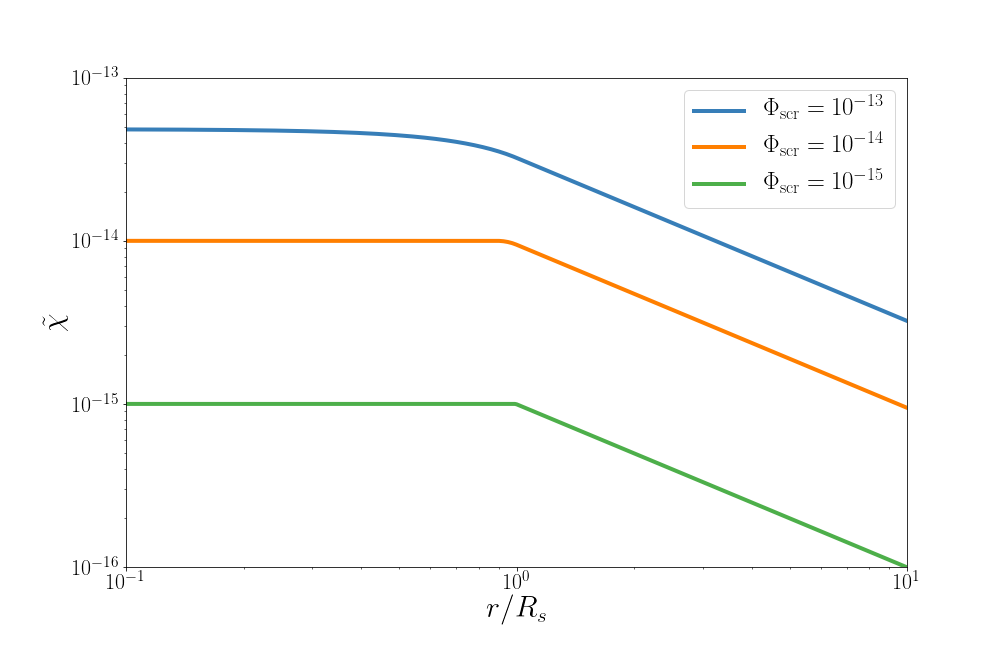
\includegraphics[width=1.0\linewidth]{{spherical_cham/starlike}.png}
	\caption{Chameleon profile for~several screening potentials. The~top solution is in~the~linear regime and~is identical to~the~gravitational potential. The~other two solutions are in~the~screened regime and~the~amplitude of~the~field is suppressed.}
	\label{fig:starlike}
\end{figure}

Let us focus on~the~regime which cannot be treated analytical, i.e. regime between thin-shell and~thick-shell solutions. This regime corresponds to~the~situation when the~linear approximation (thick-shell) breaks down inside the~object, i.e. the~gravitational potential cancels screening potential somewhere inside the~object. We will denote $\Req$ the~\textit{equivalence radius} -- radius at~which the~Newtonian potential equals the~screening potential $|\Phi_G(\Req)|=\Phi_s$. By letting the~equivalence radius posses also negative values such as $(1+|\Req|/R_s)|\Phi_G(0)|=\Phi_s$ we can clearly distinguish between the~linear $(\Req<0)$ and~the~screening $(\Req>0)$ regime.

In~\autoref{fig:starlike_forces} we show the~behavior of~the~chameleon fifth force in~this regime. We see that for~the~linear regime the~fifth force is as strong as standard gravity (up to~the~factor $2\beta^2$). For~$\Req\ll R_s$ the~chameleon field manages to~catch up with~the~linear solution inside the~object and~there is no screening outside. As the~$\Req$ grows the~field is not able to~catch up with~the~linear solution while inside the~object and~the~force outside is screened.
\begin{figure}
	\centering
	
\includegraphics[width=1.0\linewidth]{{spherical_cham/starlike_forces}.png}
	\caption{Chameleon force relative to~the~standard gravitational force for~several screening potentials (given through the~equivalence radius). For~$\Req\ll R_S$ there is no screening outside the~object. As the~$\Req$ grows the~chameleon enters the~screened regime.}
	\label{fig:starlike_forces}
\end{figure}

\subsubsection{NFW Halo}
The~Navarro-Frenk-White (NFW) profile proposed by \textcite{1996ApJ...462..563N} describes the~distribution of~cold dark matter. The~NFW profile of~matter overdensity is given by
\eq{
	\label{NFW_rho}
	\delta\rho_{\rm NFW}(r)=\frac{\rho_c}{r/r_s\left(1+r/r_s\right)^2},
}
where $\rho_c$ is the~density scale and~$r_s$ is the~scale radius. We will also be using the~dimensionless radius $x\equiv r/r_s$. The~total mass of~the~halo is divergent (logarithmically) so we take a~cut-off at~the~radius $r_{200}$, which is defined as the~radius at~which the~density is 200 times the~critical density. Then the~mass of~the~halo is
\eq{
	M_{200}=\int_0^{r_{200}}4\pi r^2\rho(r)\dd r=4\pi\rho_cr_s^3\left(\ln(1+c)-\frac{c}{c+1}\right),
}
where $c\equiv r_{200}/r_s$ is the~concentration of~the~halo. For~a~given mass the~halo is fully characterized by the~concentration.

For~NFW halo the~density is not constant as in~the~case of~compact spherical objects (stars). The~chameleon mass and~the~screened solution are therefore also not constant and~one does not have analytical solutions as in~the~case of~stars. However, for~realistic halo, the~density varies on~scales much larger than the~Compton wavelength of~the~chameleon. In~such cases, we can treat the~field as frozen in~the~same sense as in~the~case of~stars. Therefore we expect the~chameleon field to~behave in~a~similar way as in~the~case of~stars, i.e. to~follow the~Newtonian potential in~the~linear case and~to~have screened behavior for~more massive halos.

In~\autoref{fig:nfwlike_forces} we show the~chameleon fifth force. We see that the~behavior is indeed similar to~stars although the~field catches up much later. This is because there is no sudden drop in~density (and~mass of~the~field) where the~chameleon can start to~behave as free but rather the~mass is slowly dropping. This indicates that it will be much harder to~detect the~chameleon fifth force on~scales of~galaxies than for~star-like objects. This is of~course true only assuming the~screening potential is the~same on~all scales.
\begin{figure}
	\centering
	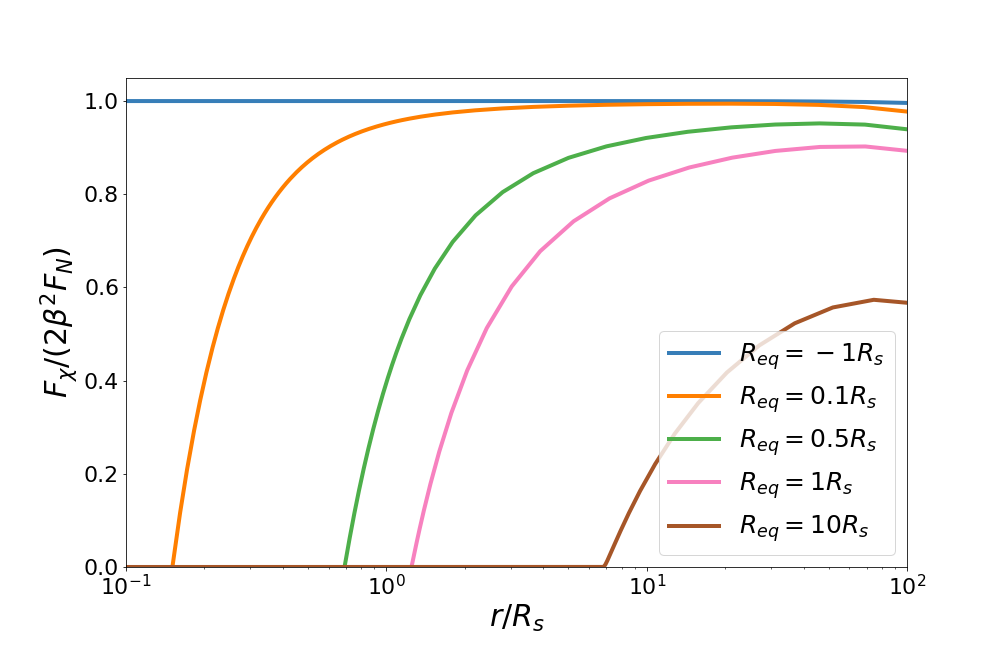
\includegraphics[width=1.0\linewidth]{{spherical_cham/nfwlike_forces}.png}
	\caption{Chameleon force relative to~the~standard gravitational force for~several screening potentials (given through the~equivalence radius). For~$\Req\ll R_S$ there is no screening outside the~object. As the~$\Req$ grows the~chameleon enters the~screened regime.}
	\label{fig:nfwlike_forces}
\end{figure}

The~meaning of~the~screening potential and~its connection to~the~Newtonian potential in~\eqref{eq:chi__scr_mean} is given by the~value of~the~field at~the~background, i.e. value that minimizes right side of~\eqref{eq:cham_u}. However, objects like stars or galaxy halos do not sit directly in~the~overall average density of~the~universe but rather in~galaxy halo or halo of~the~cluster of~galaxies. Therefore the~value of~the~effective screening potential is given by the~density of~the~background object we can consider as being in~infinity relative to~the~scale of~the~studied object. In~\autoref{fig:nfwlike_pot_eff} we show the~value of~this effective screening potential for~a~cluster of~galaxies of~a~typical size -- $M=10^{14} M_\odot, c=4$. We see that the~screening potential is greatly reduced in~inner parts of~the~galaxy cluster halo. For~this reason, we do not think it much likely to~observe the~effects of~the~chameleon field on~scales smaller than Mpc.

\begin{figure*}
	\centering
		\begin{subfigure}{1.0\linewidth}
			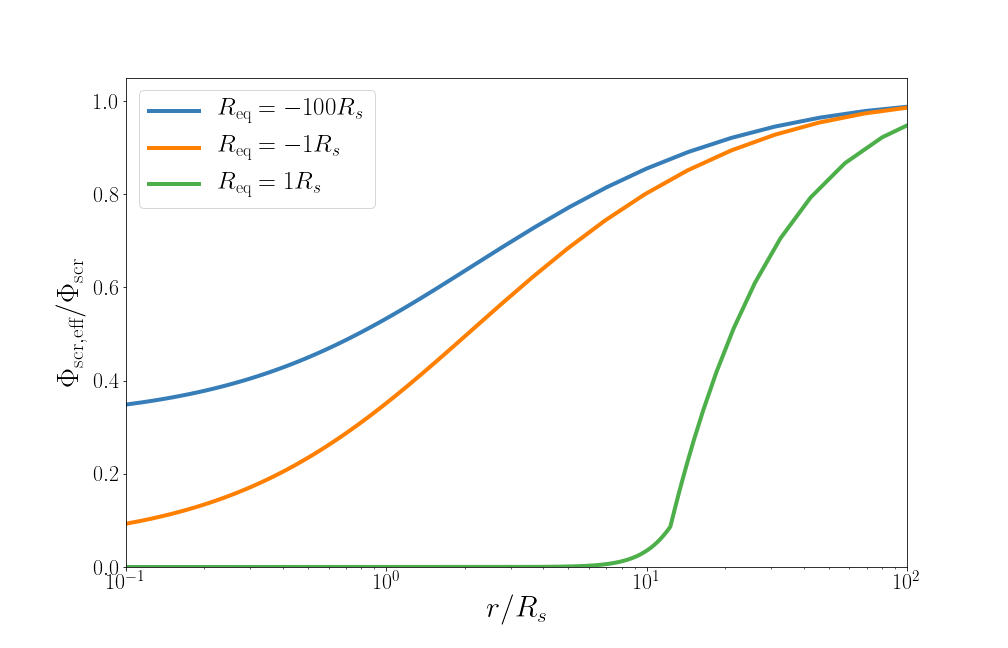
\includegraphics[width=1.0\linewidth]{{spherical_cham/nfwlike_pot_eff}.png}
		\end{subfigure}
		\begin{subfigure}{1.0\linewidth}
			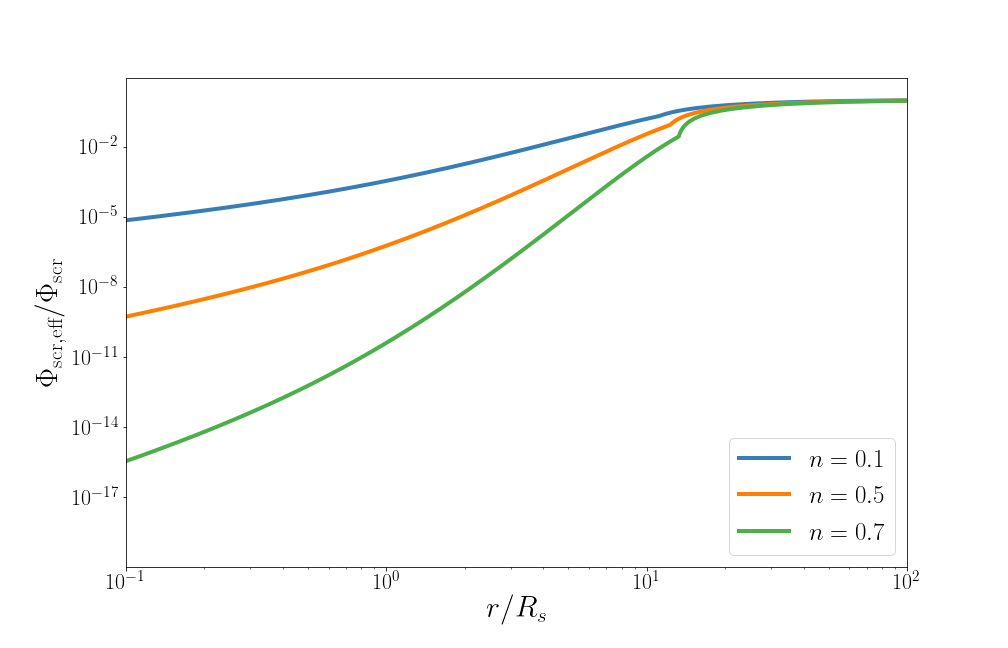
\includegraphics[width=1.0\linewidth]{{spherical_cham/nfwlike_pot_eff_n}.png}
		\end{subfigure}
		\caption{Effective screening potential relative to~the~screening potential for~a~cluster of~galaxies, $M=10^{14} M_\odot, c=4$. The~top Figure is shown for~several screening potentials (given through the~equivalence radius) while the~bottom for~different chameleon parameter $n$.}
		\label{fig:nfwlike_pot_eff}
\end{figure*}

As the~chameleon affects only non-relativistic matter it can be detected using a~combination of~dynamical measurements and~lensing measurements. Therefore, we considered what would be the~difference between the~mass distribution of~a~galaxy cluster measured via lensing (true mass) and~via dynamics of~enclosed galaxies. In~\autoref{fig:clustersYs} we plot this ratio for~five real clusters (simulated as having ideal NFW profile), see their parameters in~\autoref{tab:clusters}, and~for~four different values of~the~screening potential. We see that except for~the~case $\Phiscr=1$ one would need very precise (and~nowadays unrealistic) measurements of~the~mass distribution. We are therefore left with~only cosmological scales of~tens of~Mpc and~larger to~study the~chameleon. We will study this case in~\autoref{chpt:app_sims}.
\begin{table}[hbt]
	\centering
	\begin{tabular}{lcc|lcc}
		\hline \hline
		Cluster & $c$ & $M$ & Cluster & $c$ & $M$ \\
		\hline
		ClG 0054-27 & $1.2$ & $0.42\cdot10^{14}$ &
		Cl 0016+1609 & $2.1$ & $1.12\cdot10^{14}$ \\
		MS 2137.3-2353 & $13$ & $2.9\cdot10^{14}$ &
		ClG 2244-02 & $4.3$ & $4.5\cdot10^{14}$ \\
		MS 0451.6-0305 & $5.5$ & $18\cdot10^{14}$ & & & \\
		\hline \hline
	\end{tabular}
	\caption{Properties of~clusters simulated as perfect NFW halos: concentration $c$ and~mass $M [M_\odot]$. Parameters are taken from \textcite{2007MNRAS.379..190C}}
	\label{tab:clusters}
\end{table}

\begin{figure*}[!hbt]
\begin{adjustwidth}{-1cm}{-1cm}
	\centering
		\begin{subfigure}{0.5\linewidth}
			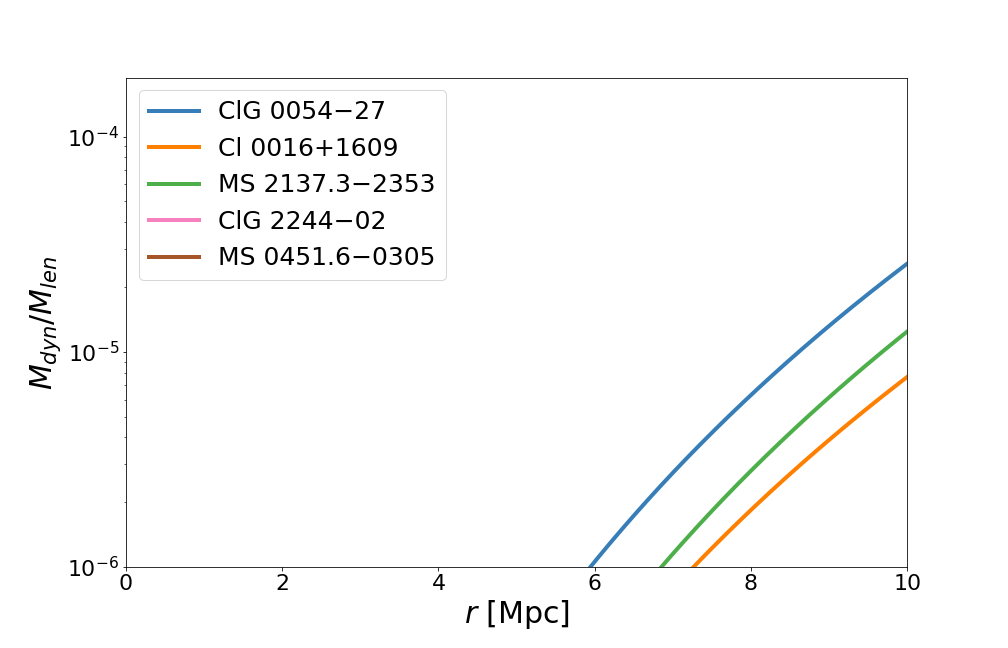
\includegraphics[width=1.0\linewidth]{{spherical_cham/clustersYs_-6}.png}
			\caption{$\Phiscr=10^{-6}$}
		\end{subfigure}
		\begin{subfigure}{0.5\linewidth}
			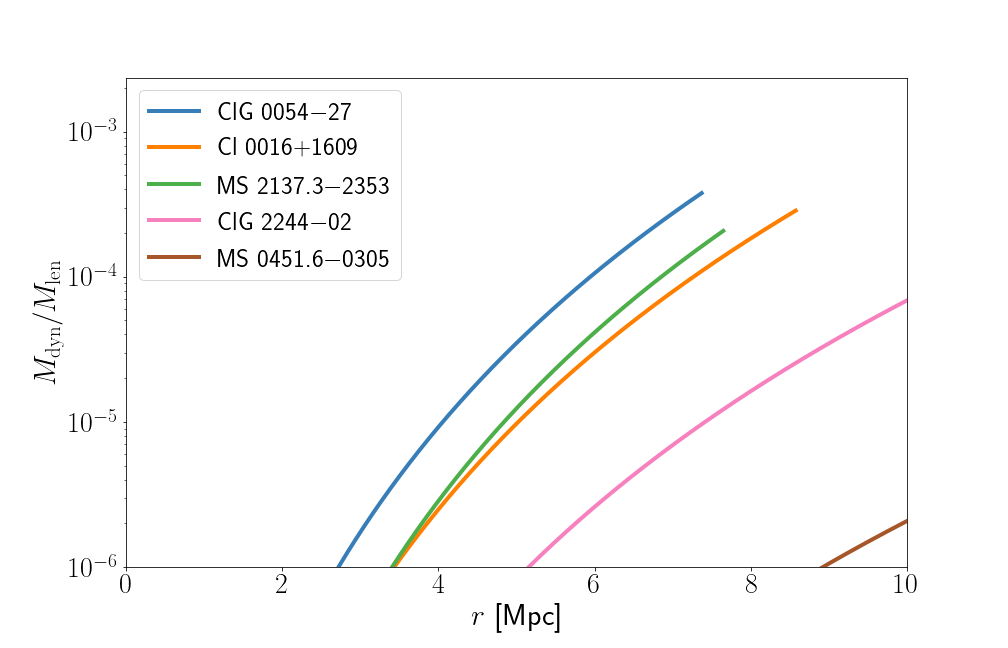
\includegraphics[width=1.0\linewidth]{{spherical_cham/clustersYs_-4}.png}
			\caption{$\Phiscr=10^{-4}$}
		\end{subfigure}
		\begin{subfigure}{0.5\linewidth}
			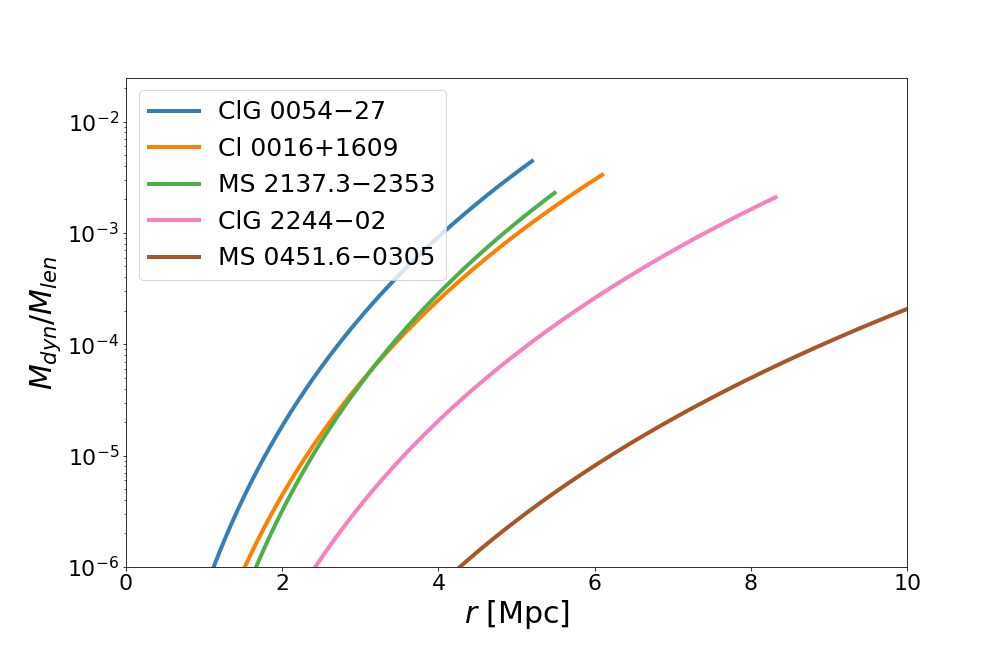
\includegraphics[width=1.0\linewidth]{{spherical_cham/clustersYs_-2}.png}
			\caption{$\Phiscr=10^{-2}$}
		\end{subfigure}
		\begin{subfigure}{0.5\linewidth}
			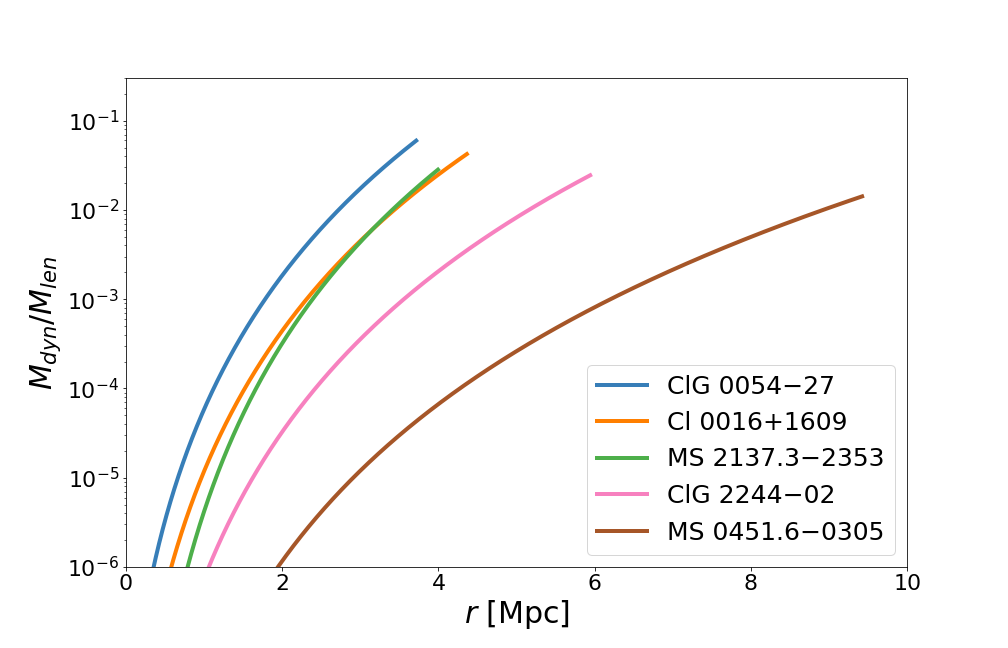
\includegraphics[width=1.0\linewidth]{{spherical_cham/clustersYs_0}.png}
			\caption{$\Phiscr=10^{0}$}
		\end{subfigure}
	\end{adjustwidth}
		\caption{Effective dynamical mass of~the~clusters relative to~the~actual (lensing) mass of~the~cluster. Cluster properties are shown in~\autoref{tab:clusters}.}
		\label{fig:clustersYs}
\end{figure*} 
\section[Other theories]{Other theories\footnote{Some parts of this section have already been published in \textcite{mastersthesis_vrastil}. The overtaken text is written in italics.}}
\label{sec:other}
In~this section we briefly mention some of~the~other theories od modified gravity. This list is in~no way complete and~serves only as an~example of~different approaches to~modifications of~gravity. See references for~further reading.
\subsection{Quintessence}
Quintessence, from the~Latin ``fifth element'', is according to~ancient and~medieval philosophy the~fifth element, or ether, supposed to~be the~constituent matter of~the~heavenly bodies after air, fire, earth, and~water. The~name quintessence, or the~$Q$ component, was first used by \textcite{1998PhRvL..80.1582C} for~the~canonical scalar field $\phi$ evolving along a~potential $V(\phi)$. Such a~dynamical field can reproduce the~late-time acceleration with~the~equation of~state $w=w(t)\approx1$. Although quintessence can alleviate the~coincidence problem of~dark energy via the~so-called tracker solution, it still suffers by the~fine-tunning problem as the~potential needs to~be flat enough to~lead to~the~slow-roll inflation today with~an~energy scale $\rho_{DE}\simeq10^{-120}\Mpl^4$ and~a~mass scale $m_\phi\lesssim10^{-33}$ eV. However, such fine-tuned potentials can be constructed within the~framework of~particle physics.

Quintessence is one of~the~simple models of~dark energy as it is a~canonical scalar field that interacts with~all the~other components only through standard gravity. The~Lagrangian density for~the~quintessence field is
\eq{
\label{Qlagr}
\LL_\phi=-\frac12(\partial\phi)^2-V(\phi)
}
We can compute the~stress-energy tensor as
\eq{
T^\phi_\uv\equiv\frac{-2}{\dg}\frac{\delta(\dg\LL_\phi)}{\delta g^\uv}=\partial_\mu\phi\partial_\nu\phi-g^\uv\left(\frac12(\partial\phi)^2+V(\phi)\right).
}
Now, the~energy density and~pressure are given by components of~the~stress-energy tensor. For~FLRW background and~$\phi$ only time-dependent we get
\eq{
\rho_\phi=-T^0_0=\frac{1}{2}\dot{\phi}^2+V(\phi)\ \ \ \ p_\phi=\frac{1}{3}T^i_i=\frac{1}{2}\dot{\phi}^2-V(\phi).
}
Equation of~state for~the~quintessence is then
\eq{
\label{eosQ}
w\equiv\frac{p}{\rho}=\frac{\dot{\phi}^2-2V(\phi)}{\dot{\phi}^2+2V(\phi)}\,.
}
We require the~condition $w<-1/3$ to~realize the~late-time cosmic acceleration, which translates into the~condition  $\dot{\phi}^2<V(\phi)$, i.e. the~potential needs to~be shallow enough for~the~field to~evolve slowly along the~potential. For~a~slow-rolling field such as $\dot{\phi}\ll V(\phi)$ equation of~state \eqref{eosQ} reduce to~$w\approx-1$ as indicated by cosmological measurements.

The~variation of~\eqref{Qlagr} with~respect to~$\phi$ gives us the~equation of~motion for~the~scalar field $\phi$
\eq{
\ddot{\phi}+3H\dot{\phi}^2+V_{,\phi}=0\,.
}

Depending on~which term and~when determines the~evolution of~the~field, the~quintessence models have been dynamically classified into \textit{freezing} models and~\textit{thawing} models \parencite{2005PhRvL..95n1301C}. In~the~freezing models the~field was rolling along the~potential in~the~past, but the~movement gradually slows down as the~field approaches the~minimum of~the~potential $(\dot{\phi}\rightarrow0)$ and~the~system enters the~phase of~the~cosmic acceleration $(w\rightarrow-1)$. In~the~thawing models, the~field was initially frozen $(\dot{\phi}\approx0)$ in~the~early matter era because of~the~Hubble friction (the~term $H\dot{\phi}$) until recently and~then it begins to~evolve once $H$ drops below $m_\phi$ and~$w$ evolves from $-1$.

A~potential of~the~freezing models is for~example
\eq{
\label{Qtr}
V(\phi)=M^{4+n}\phi^{-n}\ (n>0),
}
which appears in~the~fermion condensate model as dynamical supersymmetry breaking \parencite{1999PhRvD..60f3502B}. This potential does not possess a~minimum and~hence the~field rolls down the~potential toward infinity. Another example of~potential in~the~freezing models is
\eq{
V(\phi)=M^{4+n}\phi^{-n}\exp{(\alpha\phi^2/\Mpl^2)},
}
which can be constructed in~the~framework of~supergravity \parencite{1999PhLB..468...40B}. This potential has a~minimum at~which the~field is eventually trapped (corresponding to~$\dot{\phi}=0$ and~hence $w=-1$).

The~broader class of~potentials belonging to~the~thawing models are so-called hilltop quintessence models \parencite{2008PhRvD..78l3525D}, in~which the~scalar field is rolling near a~local \textbf{maximum} in~the~potential but it begins to~roll down around the~present. A~particular example that is well-described by this model is the~pseudo-Nambu-Goldstone Boson (PNGB) model of~\textcite{1995PhRvL..75.2077F}, for~which the~potential is given by
\eq{
V(\phi)=M^{4}\left[\cos{(\phi/f)}+1\right].
}
\subsection{K-essence}
Quintessence models are based on~a~scalar field with~a~canonical kinetic term and~a~slowly varying potential. However, in~the~context of~particle physics there appear scalar fields with~non-canonical kinetic terms. In~\textcite{1999PhLB..458..209A} it is shown that a~large class of~scalar fields with~non-canonical kinetic terms can, without the~help of~potential terms, drive an~inflationary evolution starting from rather generic initial conditions. The~Lagrangian density for~the~k-essence is
\eq{
\label{Klagr}
\LL_K=P(\phi, X),
}
where $X=-\frac12(\partial\phi)^2$ is the~canonical kinetic energy and~the~function $P(\phi, X)$ must vanish for~$X\rightarrow0$ (otherwise there would be some potential term). 

The~energy-momentum tensor of~the~k-essence is given by
\eq{
T^K_\uv\equiv\frac{-2}{\dg}\frac{\delta(\dg\LL_K)}{\delta g^\uv}=P_{,X}\partial_\mu\phi\partial_\nu\phi+g^\uv P,
}
which is of~the~form of~a~perfect fluid, $T_\uv=(\rho+p)u_\mu u_\nu+g_\uv p$, with~a~four-velocity $u_\mu=\partial_\mu\phi/\sqrt{2X}$, pressure $p_K=P$ and~energy density
\eq{
\rho_K=2XP_{,X}-P.
}
The~equation of~state of~the~k-essence is then
\eq{
w_K=\frac{p_K}{\rho_K}=\frac{P}{2XP_{,X}-P},
}
which is $w_K\approx-1$, as long as the~condition $XP_{,X}\ll P$ is satisfied.

In~the~low-energy effective string theory appear higher-order derivative terms coming from $\alpha$ and~loop corrections to~the~tree-level action \parencite{2003PhR...373....1G}. The~k-essence action for~these theories is for~example
\eq{
P=K(\phi)X+L(\phi)X^2.
}
Phantom or ghost scalar fields with~a~negative kinetic energy $-X$ and~$w\lesssim-1$ can also fit the~current observations. These ghost fields generally suffer from a~quantum instability problem unless higher-order terms in~$X$ or $\phi$ are taken into account in~the~Lagrangian density \parencite{2010deto.book.....A}. The~action of~the~so-called dilatonic ghost condensate model is \parencite{2004JCAP...07..004P}
\eq{
P=-X+e^{\kappa\lambda\phi}X^2/M^4.
}
\subsection{Gauss-Bonnet Dark Energy Models}
In~\fR\ gravity one adds the~general function of~the~Ricci scalar. But in~principle, one can add general functions of~the~Ricci and~Riemann tensors as well, e.g. $f(R,R_\uv R^\uv,R_{\alpha\beta\gamma\delta}R^{\alpha\beta\gamma\delta},...)$ \parencite{2005PhRvD..71f3513C}. These Lagrangians are generally plagued by the~existence of~ghosts.  However, there exists a~combination of~Ricci and~Riemann tensors that keeps the~equations at~second-order in~the~metric and~does not necessarily give rise to~instabilities -- so-called Gauss-Bonnet term $\GB$ coupled to~a~scalar field
\eq{
\GB\equiv R^2-4R_\uv R^\uv+R_{\alpha\beta\gamma\delta}R^{\alpha\beta\gamma\delta}.
}
The~Gauss-Bonnet term is the~unique invariant for~which the~highest (second) derivative occurs linearly in~the~equations of~motion and~thus ensuring the~uniqueness of~solutions. The~Gauss-Bonnet term naturally arises as a~correction to~the~tree-level action of~low-energy effective string theories \parencite{2000PhR...337..343L}. The~starting action is given by
\eq{
S=\int\dd^4x\dg\left[\frac{\Mpl^2}{2}R-\frac{\gamma}{2}\left(\nabla\phi\right)^2-V(\phi)+f(\phi)\GB\right],
}
where $\gamma=\pm1$ (+1 for~the~canonical scalar). For~more details see \textcite{2005PhRvD..71l3509N,2006JCAP...06..004N,2013PhRvD..87h4037C}.
\subsection{Braneworld Models}
In~the~braneworld model of~Dvali, Gabadadze, and~Porrati \parencite[DGP model][]{2000PhLB..485..208D} the~3-brane is embedded in~a~Minkowski bulk spacetime with~infinitely large extra dimensions. The~theory gives rise to~the~correct 4D potential at~short distances whereas at~large distances the~potential is that of~a~5D theory. The~action of~the~theory is
\eq{
S=\frac{M^3_{(5)}}{2}\int\dd^5X\dgt\tR+\frac{\Mpl^2}{2}\int\dd^4x\dg R + \int\dd^4x\dg \LL_m,
}
where $g_{AB}(X)=g_{AB}(x,y)$ denotes a~5D metric for~which the~5D Ricci scalar is $\tR$ and~$M_{(5)}$ is the~5D Planck mass. Capital letters are used for~5D quantities $(A,B=0,1,2,3,5)$. The~brane is located at~$y=0$. The~induces 4D metric on~the~brane is denoted by
\eq{
g_\uv(x)\equiv\tilde{g}_\uv(x,y=0).
}
The~cross-over scale $r_0$ is defined by
\eq{
r_0\equiv\frac{\Mpl^2}{2M^3_{(5)}}.
}
At~short distances $r\ll r_0$ gravity behaves as usual 4D theory, i.e the~gravitational potential has correct $1/r$ behavior (except small logarithmic repulsion term). On~the~other hand at~large distances $r\gg r_0$ the~potential scales as $1/r^2$ according to~the~laws of~5D theory.

The~presence of~the~extra dimension has severe consequences on~the~cosmology as well. It can be shown \parencite{2010deto.book.....A,2009PhLB..674..237M} that the~matter-dominated Universe approaches the~de Sitter solution $H=r_0\mins$. This cosmological solution drives our Universe into the~self-inflationary regime without dark energy. From $H_0\approx r_0\mins$ we get $M_{(5)}\approx10-100$ MeV.
\subsection{Massive Gravity}
The~idea to~give a~mass to~the~graviton (infrared modification of~gravity) is not new and~has been investigated since the~first years of~General Relativity. It is a~less minimal theory than \fR\ theories or modified gravities with~an~extra scalar field because it introduces three new degrees of~freedom rather than one. By giving a~mass $m$ to~the~graviton we deform the~classical potential to~the~Yukawa profile $\sim\frac1r e^{-mr}$ which departs from the~classical one at~distances $r>1/m$. By choosing the~graviton mass to~be of~the~order of~the~Hubble constant $m\sim H$ one can hope to~explain the~acceleration of~the~universe without dark energy.

The~simplest theory for~a~non-self-interacting massive graviton is the~Fierz-Pauli theory of~\textcite{1939RSPSA.173..211F}. The~action for~a~single massive spin 2 particle in~flat space, carried by a~symmetric tensor field $h_\uv$ is
\eq{
\begin{split}
S=&\int\dd^4x\Big[-\frac12\partial_\lambda h_\uv\partial^\lambda h^\uv+\partial_\mu h_{\nu\lambda}\partial^\nu h^{\mu\lambda}-\partial_\mu h^\uv\partial_\nu h \\
&+\frac12\partial_\lambda h \partial^\lambda h-\frac12 m^2\left(h_\uv h^\uv-h^2\right)\Big]+S_m.
\end{split}
}
Any other combination of~$h_\uv h^\uv$ and~$h^2$ would lead to~instabilities. Varying the~action with~respect to~$h_\uv$ yields the~equation of~motion
\eq{
R_\uv-\frac12Rg_\uv+\frac12m^2(h_\uv-h\eta_\uv)=\frac{1}{\Mpl^2}T_\uv,
}
where all quantities are linearized around $\eta_\uv$.

Because of~the~so-called vDVZ discontinuity (``van Dam-Veltman-Zakharov'') in~the~propagator of~a~graviton, the~Fierz-Pauli theory leads to~different physical predictions from those of~GR regardless the~mass of~the~graviton (even when $m\to0$). The~Vainshtein mechanism \parencite{1972PhLB...39..393V} allows in~principle to~get rid of~the~vDVZ discontinuity by introducing non-linear Fierz-Pauli gravity.

The~Vainshtein mechanism is another example of~the~screening mechanism and~restores the~continuity with~GR on~scales below the~so-called Vainshtein radius $r_V$, defined as
\eq{
r_V\equiv(GM/m^4)^{1/5}.
}
Much below the~Vainshtein radius, which grows as the~graviton's mass approaches $0$, only linear terms play a~crucial role and~the~GR is restored.

For~more about the~massive gravity and~the~Vainshtein mechanism see e.g. \textcite{2013CQGra..30r4001B,2012RvMP...84..671H}.

\subsection{Acceleration without Dark Energy}
So far we studied some kind of~dark energy -- either in~the~form of~an~exotic matter or by modifying gravity itself. But this need for~dark energy as an~explanation of~the~acceleration comes from our observations which are based on~the~presumption of~the~homogeneous and~isotropic Universe. What we observe are different expansion rates at~different distances rather than an~increase in~the~expansion rate at~all distances. But this can be caused by strong inhomogeneities in~the~distribution of~matter rather than by an~accelerating Universe.
\subsubsection{Void models}
The~basic idea behind void models is that we live in~the~middle of~a~huge spherical region which is expanding faster because it is emptier than the~outside. That means that the~Universe as a~whole does not accelerate but that we observe an~\textit{apparent} cosmic acceleration. The~edge of~this void should be located around $z\sim0.3-0.5$, the~value at~which in~the~standard interpretation we observe the~beginning of~the~acceleration. These models are described by the~Lema\^\i tre-Tolman-Bondi (LTB) spherically symmetric metric -- the~generalization of~a~FLRW metric in~which the~expansion factor along the~radial coordinate is different relative to~the~surface line element $\dd\Omega^2$ \parencite{2013JCAP...02..047D,2006PhRvD..73h3519A}.

The~inhomogeneous LTB model matches to~the~supernovae data and~the~location of~the~first acoustic peak of~the~CMB temperature power spectrum but cannot satisfactorily reproduce the~entire CMB angular power spectrum \parencite{2011JCAP...02..013C}. The~observed isotropy of~the~CMB radiation implies that we must live close to~the~center of~the~void -- nearer than 15 Mpc \parencite{2006PhRvD..74j3520A}. Moreover, there is no valid mechanism at~present to~explain the~formation of~such huge inhomogeneities, let alone one with~our Galaxy near the~center.
\subsubsection{Backreaction}
Unlike the~void models, which regard the~acceleration as an~apparent one, \textit{backreaction} models try to~explain the~cosmic acceleration by arranging inhomogeneities so that the~deviation from the~FLRW metric can produce a~real acceleration \parencite{2011CQGra..28w5002S,2004JCAP...02..003R,2005PhRvD..72b3507M}. Because GR equations are non-linear, averaging the~inhomogeneities and~then solving the~GR equations (which is the~usual approach) is not the~same as first solving the~full (inhomogeneous) GR equations and~then averaging them -- the~expected value of~a~non-linear function is not the~same as the~non-linear function of~the~expected value.

Any large inhomogeneities must be concealed from our sight to~fit observations. Strong peculiar velocities instead of~strong density fluctuations can do this job, but there are strong constraints on~peculiar velocities from e.g., the~kinematic Sunyaev--Zel'dovich effect. Moreover, the~accompanying anisotropy is another source of~observable effects difficult to~accommodate with~current observations.

\section{Parametrization of~models}
We saw in~the~previous chapter that at~the~background level the~evolution is governed by Friedman equations \eqref{eq:Friedmann} -- \eqref{eq:Friedmann-continuity} and~consequently omega parameters \eqref{eq:omega} and~Hubble parameter $H$ which can be obtained, e.g., from distance measurements. As we discussed, the~cosmological constant is not the~only possible explanation of~the~accelerated expansion and~the~equation of~state \(w\) of~dark energy does not have to~be exactly \(w=-1\). For~the~arbitrary equation of~state $w_{DE}=p_{DE}/\rho_{DE}$ in~the~flat Universe with~a~negligible contribution of~radiation we can obtain the~following equation
\eq{
    \label{eq:w_de}
    w_{DE}(z)=\frac{(1+z)(E^2(z))'-3E^2(z)}
                   {3\left[E^2(z)-\Omega_{m,0}(1+z^3)\right]}\,,
}
where a~prime denotes derivative with~respect to~\(z\). We see that \(w_{DE}\) cannot be determined solely from \(E(z)\) (obtainable through distance measurements) and~we need also present density of~matter \(\Omega_{m,0}\). However, if we parametrize \(w_{DE}\) in~some way as it is usually done through measurements of~\(E(z)\) at~several redshifts we can constraint both \(w_{DE}\) and~\(\Omega_{m,0}\).

Several parametrization  of~\(w_{DE}\) have been proposed so far. We can write such parametrization  in~the~form
\eq{
    w_{DE}=\sum_{n=0}w_nx_n(z)\,,
}
where he expansions can be given by
\eq{
    & \rm{(i) Redshift:}      & x_n(z) &= z^n\,, \\
    & \rm{(ii) Scale factor:} & x_n(z) &= (1-a)^n=\left(\frac{z}{1+z}\right)\,, \\
    & \rm{(iii) Logarithmic:} & x_n(z) &= \left[\ln\left(1+z\right)\right]^n\,.
}
Parametrization (ii) is usually written for~\(n\leq1\) as \(w=w_0+w_a(1-a)\).

For~the~generic \fR\ gravity, the~equation of~state is given by \parencite{2013qopu.conf...73B}
\eq{
    w_{DE} = \frac{-(1/2)(F\R R-F)+\ddot F\R+2H\dot F\R-(1-F\R)\left(2\dot H + 3H^2\right) }
                  {(1/2)(F\R - F) - 3H\dot F\R + 3 (1-F\R)H^2}\,,
}
which then can be compared with~observations \eqref{eq:w_de}. For~different examples of~evolution of~$w_{DE}$ see, e.g., \textcite{2020arXiv200707717A}. \clearpage{}
\clearpage{}\chapter{Cosmological Simulations}
\label{chpt:cosmo_sim}
In~this chapter, we will describe methods and~techniques that are used for~studying our Universe on~the~largest scales by using numerical simulations. We will describe how we implemented these methods in~our code for~\nbodysim s.

In~this chapter we will use the~following notation: box size $L$ [$\Mpch$], number of~particles $\Np$, number of~force mesh points $\Nf$, number of~power spectrum mesh points $\Na$, number of~runs $N$, number of~time-steps $\Nt$, and~a~derived parameter, the~particle mass $m$ $[M_\odot]$. This notation is summarized in~\autoref{tab:sim_param}.

\begin{table}
\centering
\begin{tabular}{ll}
    \hline \hline
    Symbol & Definition \\
    \hline
    $L$ & box size in~units of~$\Mpch$ \\
    $\Np$ & number of~particles \\
    $\Nf$ & number of~force mesh points \\
    $\Na$ & number of~power spectrum mesh points \\
    $N$ & number of~runs \\
    $\Nt$ & number of~time-steps \\
    $m$ & particle mass in~units of~$[M_\odot]$ \\
    \hline \hline
\end{tabular}
\caption{Summary of~symbols used for~simulation parameters.}
\label{tab:sim_param}
\end{table}


\section{\nbody\ problem}
Many problems in~physics, including cosmology, involve particle systems with~each particle interacting with~all other particles present. In~astronomy, there is a~gravitational interaction between stars, galaxies, and~cluster of~galaxies, depending on~the~scale which we are studying. The~challenge of~efficiently carrying out the~related calculations is generally known as the~\nbody\ problem.

The~main problem is the~following -- we have $N_p$ particles all interacting gravitationally with~each other. To~compute a~trajectory of~even a~single particle involves computing trajectories of~all other particles as the~gravitational force is dependent the~on~time-varying positions of~other particles. That means that at~each time-step we have to~compute forces from all other $N_p$ particles and~we need to~compute these forces for~each of~$N_p$ particles. This leaves us with~complexity of~\(\OO(N_p^2)\). This brute force approach can be used only for~small systems and~is computationally unimaginable for~large systems in~cosmology which typically involve \(N_p\sim10^{9}\) particles.

This direct approach is generally referred to~as the~Particle-Particle (PP) method \parencite{Hockney:1988:CSU:62815}. Although computationally expensive the~accuracy in~the~force calculation is of~machine precision. To~be able to~simulate large systems of~particles we need to~drop the~accuracy of~continuous positions and~use discrete positions for~force calculations. In~our code, we use two main methods for~force calculations -- the~Particle-Mesh algorithm (PM) and~grid-based methods, both of~them we describe in~more detail below.
\subsection{Time integration}
Accurate time integration is a~very important part of~any \nbodysim. While there are many different methods to~integrate particle trajectories \parencite[see e.g.][]{Hockney:1988:CSU:62815} we describe here one of~the~most used ones in~collisionless simulations -- the~Leapfrog integrator.

The~leapfrog integrator belongs to a~class of~symplectic integrators \parencite{2011EPJP..126...55D}. Symplectic integrators are canoncial transformations and as such, they conserve certain quantities such as the~total angular momentum, the~phase-space volume, and~the~Jacobi constants. Instead of solving the~exact Hamiltonian approximately, the~leapfrog integrator tries to solve an approximate Hamiltonian exactly
\eq{
    \tilde H=H+H\err\,,
}
where \(H\err\) is the~error Hamiltonian. If \(\tilde H\) and~\(H\) do not dependent explicitly on time, the~error in~energy is bounded at~all times. We want to find such a \(\tilde H\) that can be solved easily by numerical methods and~simultaneously and~minimizes \(H\err\). The~Hamilton's equations are
\eq{
    \dot w=\HH w\,,
}
where \(w\equiv(x,p)\) are combined phase-space coordinates and \(\HH\equiv\{\cdot,H\}\) is an~operator acting on~\(w\) through Poisson bracket. Hamilton’s equations have then the~formal solution
\eq{
    w(t+\Delta t)=e^{\Delta t\HH}w(t)\,.
}
\begin{sloppypar}
We want~to split the~operator \(e^{\Delta t\HH}\) (approximately) into steps that, individually, can be integrated exactly. This is usually done by separating the Hamiltonian into the~kinetic and~potential energies, \({H=T(p)+V(x)}\). That we can write
\end{sloppypar}
\eq{
    \label{eq:kdk}
    e^{\Delta t\HH}= e^{\Delta t(\TT+\VV)}\approx e^{\frac12\Delta t\VV}e^{\Delta t\TT}e^{\frac12\Delta t\VV}\,,
}
where operators \(\TT\equiv\{\cdot,T\}\) and~\(\VV\equiv\{\cdot,V\}\) are known as drift and~kick, as they only change either the~positions (drift) or velocities (kick). Because these operators are non-commutative, the~central relation in~\eqref{eq:kdk} is only approximately true. This operator splitting is extremely useful because the~new equations have a~simple solution:
\eq{
    e^{\Delta t\TT}
    \begin{pmatrix}
        x \\
        p \\
    \end{pmatrix}=
    \begin{pmatrix}
        x+\Delta t\ p \\
        p \\
    \end{pmatrix}
    \mspace{20mu}\rm{and}\mspace{20mu}
    e^{\Delta t\VV}
    \begin{pmatrix}
        x \\
        p \\
    \end{pmatrix}=
    \begin{pmatrix}
        x \\
        p-\Delta t\ \nabla V \\
    \end{pmatrix}\,.
}
The~splitting \eqref{eq:kdk}, also known as kick-drift-kick (KDK), is second-order accurate, whereas simpler splitting only into one kick and~one drift is first-order accurate. The~same accuracy and~results have also similar splitting into drift-kick-drift which we use in~our integrator.
\section{Particle-Mesh algorithm}
\label{sec:PM}
As we mentioned in~the~introduction, in~order to~effectively compute forces on~particles one has to~abandon the~continuous position and~solve the~forces using discretized positions. The~idea of~the~PM method is that we set up a~mesh (grid) over the~computational box, and~then we solve the~gravitational potential (i.e. Poisson’s equation \eqref{eq:poisson_lin}) at~the~mesh-points \parencite{n_body_Lindholm}. Forces at~the~mesh-points can then be obtained by calculating the~gradient of~the~potential. The~four principal steps of~the~particle-mesh calculation are \parencite{Hockney:1988:CSU:62815}:
\begin{enumerate}
    \item assign mass to~the~mesh,
    \label{it:pm_1}
    \item solve the~field equation on~the~mesh,
    \label{it:pm_2}
    \item calculate the~mesh-defined force field,
    \label{it:pm_3}
    \item interpolate to~find forces on~the~particles,
    \label{it:pm_4}
\end{enumerate}
where the~forces found at~the~last step are used to~integrate the~equations of~motion.
\subsection{Assignment schemes}
In~step \ref{it:pm_1} and~\ref{it:pm_4} we make a~connection between discrete mesh and~continuous positions of~the~particles. In~the~first, we need to~distribute the~mass of~all particles onto the~mesh and~in~the~last step, on~the~contrary, we need to~interpolate forces known on~the~discrete mesh onto particles with~continuous positions. We can assign the~masses of particles to~the~discrete density function $\delta$ and~the~discrete force $-\nabla\Phi$ to~the~particles in several ways:

\subsubsection{Nearest gridpoint (NGP)}
The~mass of~each particle $m_i$ is assigned as a~whole to~the~gridpoint closest to~the~particle. Similarly, the~force on~particles is given by force on~the~nearest gridpoint. Although computationally the~simplest, NGP as a~zero-order interpolation offers lowest accuracy, and~the~interparticle force changes discontinuously as particles cross cell boundaries.

\subsubsection{Cloud-in-Cell (CIC)}
The~mass of~each particle is weighted over the~eight closest cells while the~weighting in~each dimension is proportional to~the~distance between the~particle and the~mesh. CIC scheme is more costly in~terms of~the~number of~arithmetic operations per particle per timestep than NGP but offers better accuracy as first-order (linear) interpolation. The~CIC interpolation function in~one dimension is
\eq{
    w(x-x_p)=
    \begin{cases}
        1-\frac{|x-x_p|}{H} & |x-x_p|<H\,\\
        0 & \rm{otherwise}
    \end{cases}
}
where $x$ is the~position of~a~mesh point, $x_p$ position of~the~particle, and~$H$ the~distance between mesh points. The~three-dimensional interpolation function is \(W(\mathbf x)=w(x_1)w(x_2)w(x_3)\). The~CIC scheme is somewhere in~the~middle between oversimplistic NGP and~higher-order interpolations which offer greater accuracy and~smoother transitions but at~the~cost of~much greater computational resources -- second-order interpolation (triangular shaped cloud, TSC) involves 27 cells, third-order 64, etc. The piecewise linear force of the CIC is much smoother than that of the~NGP scheme. It~also reduces the~amplitude of~fluctuations in~the~interparticle forces when the~particles are displaced with~respect to~the~mesh. In~our code, we use the~CIC scheme.

\subsection{Solution of~the~field equations}
An~efficient method for~the~solution of~the~field equations is a~necessary requirement for~the~practical implementation of~the~particle simulation algorithms that have been described. For~linear Poisson’s equation \eqref{eq:poisson_lin} the~most used method is the~Fast Fourier Transformation which can compute convolutions involve in~the~force computation rapidly with~the~complexity of~$\OO(N_m\log N_m)$. The~FFT also automatically solves periodic boundary conditions usually incorporated in~cosmological simulations to~enforce homogeneity and~isotropy of~the~Universe. Therefore, FFT-based methods are predominantly used with~cosmological simulations.

The~Green's function $G(k)$ of~\eqref{eq:poisson_lin} is not the~expected one, $-1/k^2$, but we have the~freedom to~choose such a~Green's function which will minimize errors introduced by all the~steps involve in~force calculation -- mass assignment, potential solver, finite difference and~force interpolation. This topic is in~great detail studied in~\textcite{Hockney:1988:CSU:62815}.
\subsection{Particle-Particle Particle-Mesh algorithm}
The~PM methods are excellent for~solving long-range forces between particles as these methods are very fast and~accurate. However, this accuracy is limited by the~mesh size $H$, and~PM algorithms cannot truly describe anything below this scale. The~accuracy is given by the~Nyquist wavelength $\lambda_N=2H$, which is the~shortest spatial wavelength that can be accurately recovered. Similarly, power on~wavenumbers larger than the~Nyquist wavenumber $k_N=2\pi/\lambda_N=N_m\pi/L$ will be aliased into longer waves. To~overcome these limitations Particle-Particle Particle Mesh algorithms (P$^3$M) have been proposed \textcite{hockney_10000_1973}.

In the P$^3$M algorithm, one writes the~interparticle force as the~sum of~the~short-range force, which is limited by some cutoff radius,and~the~long range force, which varies smoothly and~is approximately band-limited (that is to~say, is approximately nonzero for~only a~limited range of~$k$). The~short-range force on~a~particle is computed by direct particle-particle (PP) force summation and~the~longe-range force is computed using the~particle-mesh (PM) algorithm.

We do not use P$^3$M in~our approximate methods because of~their much greater numerical requirements compared to~simpler PM methods. For~more details, see e.g. \textcite{Hockney:1988:CSU:62815}.
\section{Multi-grid techniques}
Practical multi-grid techniques were introduced by \textcite{10.2307/2006422}. These methods also use the~discrete grids and continuous particles positions as PM methods based on~FFT with~$\OO(N_m\log N_m)$ complexity but they use relaxation methods such as Gauss-Seidel iteration \parencite{doi:10.1002/zamm.19720520813} and~can solve elliptic partial differential equations using $\OO(N_m)$ operations. The~speed of~these methods is comparable to the PM and other rapid methods, but the~multigrid methods can also solve general elliptic equations with~nonconstant coefficients. Even non-linear equations of~modified gravitational can be solved with~these methods \parencite{10.5555/42249}.

The~basic principle of the multigrid methods is based on the~fact, than on a~smaller (coarser) grid, we can achieve an approximate solution with small long-range errors faster than on~a~bigger (finer) grid. The~problem is sequentially transferred to~coarser and~coarser grids, each time smoothing the~errors via a~few Gauss-Seidel iterations, until~the convergence on~the~coarsest grid is achieved. The~problem is then transferred back to~finer and~finer grids, each time iterating until convergence \parencite{2011EPJP..126...55D}.
\subsection{Simple two-grid V-cycle}
Let us first consider the~simple case of~a~two-grid method. We want to~solve the~discretized linear elliptic problem on~a~uniform grid with~mesh size $h$
\eq{
    \LL_h u_h=f_h\,,
}
where $\LL$ is some linear elliptic operator and~$f$ is the~source. The~error or correction of~the~(exact) solution $u_h$ to~some approximate solution $\tilde u_h$ is
\eq{
    v_h\equiv u_h-\tilde u_h.
}
The~residual or defect is
\eq{
    \label{eq:defect}
    d_h\equiv\LL \tilde u_h-f_h\,.
}
Since $\LL_h$ is linear, the~error satisfies
\eq{
    \label{eq:residual}
    \LL_hv_h=-d_h\,.
}
To~find $v_h$ we need to~make an~approximation to~$\LL_h$. This can be done using classical iteration methods, such as Jacobi or Gauss-Seidel, which use a~simpler operator than $\LL_h$, e.g. only the~diagonal part for~the~Jacobi iteration, or the~lower triangle for~the~Gauss-Seidel iteration.

Instead of~using a~simpler form of~$\LL_h$ we can use a~coarser form, i.e. we will solve the~problem using $\LL_H$ on~a~coarser grid with~$H=2h$. The~residual equation \eqref{eq:residual} is now approximated by
\eq{
    \label{eq:residual_H}
    \LL_Hv_H=-d_H\,.
}
Since $\LL_H$ has a~smaller dimension this equation can be solved much faster than the~original fine-grid solution. To~transform residuals from fine to~the~coarse grid we need a~restriction operator $\RRR$, and~similarly, we need a~ prolongation operator $\PP$ to~interpolate corrections from coarse to~the~fine grid.
\eq{
    \label{eq:restrict}
    d_H &= \RRR d_h\,,\\
    \label{eq:prolong}
    \tilde v_h &= \PP \tilde v_H\,,
}
where $\tilde v_H$ is some approximate solution of~\eqref{eq:residual_H}. The~new approximation $\tilde u_h\new$ is then obtained as
\eq{
    \label{eq:new_app}
    \tilde u_h\new = \tilde u_h + \tilde v_h\,.
}

The~idea behind multigrid techniques is a~combination of~smoothing on~the~fine grid (relaxation) and~on~the~coarse grid (coarse-grid correction). Relaxation can rapidly reduce high-frequency errors but low-frequency errors tend to~converge slowly. On~the~other hand, high-frequency errors are not even representable on~the~coarse grid and~low-frequency errors converge much quickly. The~whole scheme, two-grid V-cycle, is thus:
\begin{itemize}
    \item Apply a~relaxation method to~$\tilde u_h$ (pre-smoothing),
    \item Compute the~defect on~the~fine grid from \eqref{eq:defect},
    \item Restrict the~defect by \eqref{eq:restrict},
    \item Solve \eqref{eq:residual_H} on~the~coarse grid,
    \item Interpolate the~correction to~the~fine grid by \eqref{eq:prolong},
    \item Compute the~next approximation by \eqref{eq:new_app},
    \item Apply a~relaxation method to~$\tilde u_h\new$ (post-smoothing).
\end{itemize}
To~achieve the~full multigrid method is now straightforward. Instead of~solving the~coarse-grid defect exactly, we can get an~approximate solution by introducing an~even coarser grid and~so on.

We considered $\LL$ to~be a~linear operator but the~above method works also with~non-linear operators. The~speed of~convergence is obviously worse and~depend on~the~exact form of~the~operator. For~our problem and~finding solutions to~the~chameleon equation of~motion \eqref{eq:cham_husa} this method proves to~be sufficient.

\subsubsection{Gauss-Seidel relaxation}
The~most popular smoothing method is Gauss-Seidel relaxation. The~Gauss-Seidel scheme for~$N_m$ mesh points is
\eq{
    \label{eq:GS}
    u_i\new = u_i -\left(\sum^{N_m}_{j\neq i}L_{ij}u_j-f_i\right)\frac{1}{L_{ii}}\,,
}
where new values of~$u$ are used on~the~right-hand side as they become available. It is usually best to~use the~tile scheme, making one pass through the~mesh updating the~even points and~another pass updating the~odd points.

For~non-linear problems as ours, one needs to~modify the~scheme \eqref{eq:GS} by Newton iteration
\eq{
    u_i\new=u_i-\frac{L_i(u_i)-f_i}{\partial L_i(u_i)/\partial u_i}\,.
}
\section{Initial conditions}
So far we have described how the~particles evolve under their mutual gravity. However, in~a~cosmological simulation, we must first place these particles into the~simulation box -- we must specify the~initial conditions (IC). The~particles cannot be placed arbitrarily but they must represent the~real Universe. Among the~properties we want is the~particles to~simulate our homogeneous, isotropic, and~infinite Universe. As we described in~\autoref{chpt:cosmo_evol} the~particles evolve and~the~resulting density field $\delta$ is not perfectly homogeneous. Statistical properties of~the~Gaussian density field, which is predicted by simple inflation models and~supported by observation, can be entirely described by the~matter power spectrum $P(k)$. Any procedure for~generating the~IC must be able to~place the~particles in~the~simulation box such as the~resulting density field retains all of~these properties.

Our code for~generating the~IC is based on~a~convolution method described by \textcite{1997ApJ...490L.127P}. We first create a~random uncorrelated Gaussian density field $n(x)$ of~unit variance. This white noise has a~constant power spectrum $\left\langle|\hat n(k)|^2\right\rangle=1$. We then convolve this field with~a~correlation kernel $W(k)=\sqrt{P(k)}$ to~obtain the~initial  density field
\eq{
    \delta(k)=n(k)W(k)\,.
}
It can be easily seen that this density field has the~correct power spectrum $\left\langle|\hat\delta(k)|^2\right\rangle=P(k)$. This density field is then used to~compute the~gravitation potential and~forces in~the~simulation box. The~actual positions and~velocities of~the~particles are found using the~linear perturbation theory, the~Zel'dovich approximation \parencite{1970A&A.....5...84Z},
\eq{
    \mb x = \mb q + D(t)\mb S(\mb q)\,,
}
\begin{sloppypar}
where $D$ is the~growth function at~the~start of~the~simulation (typically ${z\sim20-200}$). The~displacement field $S$ is computed from the~linear theory and~satisfies
\end{sloppypar}
\eq{
    \nabla\cdot \mb S = -\delta\,.
}
The~initial positions $\mb q$ of~particles are chosen to~be grid points of~the~simulation box to~satisfy homogeneity and~isotropy. We use these grid-based IC but the~so-called glass IC can also be employed. In~the~glass IC, the~particles are placed at~random positions across the~box and~then evolved with~repulsive gravity until they reach an~equilibrium state. These IC look more natural but contain lots of~white noise power.

In~order to~have reliable results, one has to~run the~cosmological simulation many times with~different IC to~lower the~sampling variance. To~accelerate the~convergence, we use each IC twice, the~second time with~opposite phases \parencite{PhysRevD.93.103519}. Opposite phases of~the~density field in~the~Fourier space correspond to~switched minima and~maxima of~the~gravitation potential in~the~real space, $n_2(\mb x)=-n_1(\mb x)$

\section{Core Cosmology Library}
The~Core Cosmology Library (\code{CCL}, \textcite{2019ApJS..242....2C}) is an~open-source software package written in~\code{C}, with~a~\code{python} interface. The~\code{CCL} provides routines to~compute basic cosmological observables such as various distances, power spectra, correlation functions, and~many others. The~accuracy of~all quantities has been extensively tested and~compared with~many other independent software packages. This allows establishing a~well-defined numerical accuracy for~each predicted quantity. The~\code{CCL} was developed for~the~needs of~the~DESC of~the~LSST which needs very precise predictions for~the~next generation of~cosmological analysis. The~author contributed to~the~development of~this library, mainly by writing documentation, examples of~usage and~helping with~automatization process and~improving its compatibility.

We use \code{CCL} for~quantities such as linear and~non-linear power spectra or growth functions. Internally, \code{CCL} calculates the~matter power spectrum  $P(k)$ using various methods including common approximations, by calling external software such as Cosmic Linear Anisotropy Solving System (\code{CLASS}, \textcite{class}), or emulators, such as the~CosmicEmu emulator \parencite{Heitmann:2015xma}.

\section{Other methods}
\subsection{TreePM}
The~tree code was pioneered by \textcite{1986Natur.324..446B} and~uses a~hierarchical spatial tree to~define localized groups of~particles. This has an~advantage over an~equidistant mesh when dealing with~highly inhomogeneous systems like stellar dynamics when few cells can contain most of~the~particles in the system. When using the~oct-tree, each cubic cell containing more than some maximum number of~particles is split into eight child cells of~half their parent's size. In~this way, a~tree-like hierarchy of~cubic nodes is created. The~particles within each of~the~tree nodes constitute a~well-defined and~localized group. The~potential of~a~cell is obtained by multipole expansion around some center of~the~group of~particles (usually center of~mass). The~gravity at~any point is then approximated by the~summation of~potentials from all other cells while considering only cells with~a~sufficiently small opening angle (size of~the~cell over the~distance). If the~opening angle is big the~same algorithm is applied to~the~daughter cells \parencite{2011EPJP..126...55D}.
\subsection{Fast multipole methods}
The~fast multipole method of~\textcite{1987JCoPh..73..325G} also works with~localized particle groups and~was originally proposed using a~fixed grid but \textcite{2000ApJ...536L..39D} implemented the~method using a~tree structure with~better results. The~method works similarly as the~tree code but in~addition to~expanding the~potential at~the~source positions, it also expands it at~the~sink positions. This speeds up the~computation of~gravity for~all particles significantly but has no advantage over the~tree methods when computing the~force at~a~single position \parencite{2011EPJP..126...55D}.

The~second part of the force calculation is the~interaction phase when the~coefficients of~the~Taylor series are evaluated for~each cell. If the~opening angle for~a~mutual cell-cell interaction is small enough the~coefficients for~the~interactions in~each direction are computed.  Otherwise, the~interaction is split into up to~8 new interactions by opening the~bigger of~the~two cells. The~total complexity of the~algorithm is given by~$\OO(N_p)$ interactions for~the~computation of~all $N_p$ particle forces. This represents a~great reduction from the~$\OO(N_p^2)$ for~direct summation and~can greatly improves simulations of~astrophysical problems with~inhomogeneous particle distributions.
%
\clearpage{}
\clearpage{}\chapter{Approximation Schemes}
\label{chpt:app_schemes}
In~this chapter we will introduce different approximation methods that we plan to~use in~our numerical simulations. We will go over equations governing their behavior and~we also briefly mention some other approximations that were used in~the~past.

Parts of~this chapter have been published in~\textcite{2020MNRAS.493.2085V}.

\section{Motivation}
Various approximations in~different scientific fields have always been studied in~detail. Many non-linear equations cannot be solved analytically and~one can hope to~achieve at~least some results using linearization or other perturbation theories of~higher-order. Cosmological simulations are no exception. From the~beginning of~first attempts to~simulate clustering of~matter on~large scales in~the~late '60s the~approximate methods were developed to~help understand the~dynamics of~the~Universe. The~greatest pioneering efforts to~improve and~validate these approximate methods have been undertaken in~the~'90s.

These analytic or semi-analytic methods can be used to~understand the~otherwise very complicated problem of~structure formation. Instead of~running a~simulation ``blindly'' and~trying to~analyze them phenomenologically one can compare these simulations with~much better understood approximate methods.

Besides the~usefulness of~approximations in~getting an~insight into gravitational evolution, they are very helpful in~getting a~large number of~simulations quickly. In~order to~study BAO, one needs a~high number of~simulations with~very large volume and~a~high number of~particles which requires demanding resources. The~BAO scale is of~particular interest to~us as it lies between the~linear regime which can be studied analytically and~the~highly non-linear regime of~halo formation which requires precise \nbodysim s. The~semi-analytical methods are expected to~work very well in~this regime.

In~this chapter, we describe several approximations that have been studied in~the~past -- Zel'dovich approximation and~its \textit{truncated} extension, frozen-flow approximation, and~frozen-potential approximation. The~Zel'dovich approximation has been studied extensively in~the~past and~here we use it mainly as a~reference for~comparison in~the~context of~the~other approximations.

\section{Recapitulation of~the~linear theory}
Here we remind some results of~the~linear theory previously presented in~\autoref{chpt:cosmo_evol}. We rewrite the~equations using variables more suited for~cosmological simulations. We will be working in~comoving coordinates -- the~comoving position $\mb x$ is defined in~terms of~the~proper position coordinate $\mb r = a\mb x$. The~comoving velocity $\mb v$ is then defined as a~derivative with~respect to~cosmic time $t$, $\mb v = \dot{\mb x}$, where the~overdot denotes a~time derivative. Particles move in~the~Newtonian gravitational potential, $\Phi$. The~equations for~linear perturbations then read
\eq{
	\label{eq:lin_per_a}
	\dot\delta + \nabla\cdot\mb v &= 0, \\
	\label{eq:lin_per_b}
    \dot{\mb v} + 2\frac{\dot a}{a} \mb v &= -\frac{1}{a^2}\nabla\Phi, \\
\begin{split}
	\label{eq:lin_per_c}
	\Delta\Phi &= 4\pi G\bar\rho a^2 \delta \\
    			&= \frac32 H_0^2\Omega_{m, 0}\frac\delta a \equiv \mu^{-1}\frac\delta a\,,
\end{split}
}
where we defined the~constant $\mu\equiv\left(\frac32 H_0^2\Omega_{m, 0}\right)^{-1}$. In~this linear regime, the~time and~space dependence of~the~overdensity evolution are separable and~we can write $\delta(a, \mb x)=D(a)\delta_0(\mb x)$ where the~growth factor $D$ represents the~growing solution (we neglect the~decaying mode) and~is normalized to~unity at~the~present time.

It is often useful to~rewrite these equations with~a~different time variable, namely the~scale factor $a$. This is convenient both from the~numerical and~theoretical points of~view because the~quantities are ``more constant''. With~the~new time-variable $a$ and~comoving velocity $\mb u = \dd \mb x/\dd a$, equation \eqref{eq:lin_per_a} becomes
\eq{
\label{eq:continuity_a}
	\dddd D a \delta_0 + \nabla\cdot\mb u = 0\,,
}
where $\dd D/\dd a = 1$ in~the~Einstein--de Sitter universe (hereafter EdS) and~so the~divergence of~the~velocity field remains constant in~both time and~space. Equation \eqref{eq:lin_per_b} then becomes
\seq{
	\label{eq:motion_EdS}
	\dddd{\mb u}{a} &= -\frac{3}{2a}\left[\mb u + \mu\nabla\Phi \right] \\
\intertext{in~EdS and, more generally,}
	\label{eq:motion_LCDM}
	\dddd{\mb u}{a} &= -\frac{3}{2a}\left[\mb u\left(1+\Omega_\Lambda\right) + \mu\nabla\Phi\left(1-\Omega_\Lambda\right)\right]
}
in~the~\LCDM\ universe. The~omega factor of~the~cosmological constant
\eq{
	\Omega_\Lambda(a) = \frac{\Omega_{\Lambda,0}a^3}{\Omega_{m,0} + \Omega_{\Lambda,0}a^3}
}
rises from $0$ to~$\Omega_{\Lambda,0}$ and~becomes significant $(>5\%)$ around redshift $z\approx2.5$. The~transformation \eqref{eins_trans} from the~Jordan frame to~the~Einstein frame introduces non-standard coupling of~the~chameleon field to~standard matter resulting in~the~fifth force \eqref{cham_force}. Using our new variables, this equation reads
\eq{
	\label{eq:cham_force}
	\dddd{\mb u_{\chi}}{a} = -\frac{3\mu}{2a}\frac{\beta}{\Mpl}\mb{\nabla}\chi \,.
}
Equation \eqref{eq:lin_per_c} expressed with~the~growth factor reads
\eq{
\label{eq:poisson_a}
	\Delta\Phi(\mb x, a) = \mu^{-1}\frac D a \delta_0(\mb x)\,.
}
\section{Zel'dovich approximation}
The~Zel'dovich approximation \parencite[hereafter ZA;][]{1970A&A.....5...84Z} bears its name after a~pioneer in~the~study of~large-scale structure, a~Soviet physicist Yakov Zel'dovich. The~ZA provides an~intuitive way to~understand the~emergence of~filamentary structures (cosmic web) and~can realize the~model of~non-linear structure formation even though it is based only on~linear approximations \parencite{2014MNRAS.439.3630W}. The~Zel’dovich approximation predicts the~rich structure of~voids, clusters, sheets, and~filaments observed in~the~Universe.

The~ZA is based on~an~ansatz that particles move in~straight lines in~the~Lagrangian frame
\eq{
\label{eq:ZA}
	\mb x(\mb q, a) = \mb q + D(a)\mb S(\mb q)\,,
}
where $\mb q$ are the~initial positions (Eulerian coordinates) of~a~particle and~$\mb S$ is some displacement field. Inserting equation \eqref{eq:ZA} into the~continuity equation \eqref{eq:continuity_a} yields
\eq{
	-\nabla\cdot S = \delta_0\,.
}
Combining with~the~Poisson equation \eqref{eq:poisson_a}, we can see that \eqref{eq:ZA} represents a~potential flow, $\mb S = -\nabla\phi_V$, where the~velocity potential $\phi_V$ obeys the~Poisson equation
\eq{
	\label{eq:poisson_vel}
	\Delta\phi_V = \delta_0
}
and~has a~simple relation to~the~gravitational potential
\eq{
	\label{eq:vel_new}
	\phi_V=\mu\frac a D \Phi\,.
}
This results to~ZA being
\eq{
	\mb x(\mb q, a) = \mb q - D(a)\mb\nabla \phi_V(\mb q)\,.
}
Note that the~velocity potential is not exactly a~potential of~our velocity field $\mb u$ but
\eq{
	\label{eq:ZA_u}
	\mb u\ZA(\mb x) = -\dddd D a \nabla\phi_V(\mb q)\,.
}
The~ZA differs from other approximations (among other things) in~how this (constant) velocity potential, $\phi_V$, enters the~equations of~motion. To~avoid having different definitions of~the~\textit{real} velocity potential for~the~velocity fields in~each approximation, we take the~equation \eqref{eq:poisson_vel} as defining the~velocity potential $\phi_V$.

The~deformation tensor is defined as
\eq{
	d_{ij}=\partpart{x_i}{q_j}=\delta_{ij}+D\partpart{\nabla_i\phi_V}{q_j}\,.
}
The~eigenvectors of~the~deformation tensor determine the~principal directions of~the~collapse and~the~corresponding eigenvalues determine the~time when the~compression will be infinite. The~density is given through eigenvalues $\lambda_i$ as
\eq{
	\rho=\frac{\bar\rho}{(1-D\lambda_1)(1-D\lambda_2)(1-D\lambda_3)}\,.
}
The~time when the~density in~ZA becomes infinite corresponds to~particles crossing the~paths of~other particles. Once this shell-crossing has occurred, the~approximation has formally broken down, since there are no forces present to~slow down the~particles and~capture them within halos.

In~\autoref{fig:slice_dens_ZA} we show a~comparison of~the~simulations with~ZA at~four different redshifts through the~projected density field. At~redshift $z=\ztwo$ the~cosmic web still looks nice but after that, at~redshifts $z=\zthree, \zfour$, we can see that shell-crossing occurred and~the~overall picture gets blurry. The~large-scale structures remain visible but the~small-scale structures get diluted at~later times.
\begin{figure*}[!htbp]
	\begin{adjustwidth}{-1cm}{-1cm}
	\centering
		\begin{subfigure}{0.5\linewidth}
			\includegraphics[width=1.0\linewidth]{{simulations_approx/dens/za_dens_512m_1p_1024M_200b_z\zone}.png}
			\caption{$z=\zone$}
		\end{subfigure}
		\begin{subfigure}{0.5\linewidth}
			\includegraphics[width=1.0\linewidth]{{simulations_approx/dens/za_dens_512m_1p_1024M_200b_z\ztwo}.png}
			\caption{$z=\ztwo$}
		\end{subfigure}
		\begin{subfigure}{0.5\linewidth}
			\includegraphics[width=1.0\linewidth]{{simulations_approx/dens/za_dens_512m_1p_1024M_200b_z\zthree}.png}
			\caption{$z=\zthree$}
		\end{subfigure}
		\begin{subfigure}{0.5\linewidth}
			\includegraphics[width=1.0\linewidth]{{simulations_approx/dens/za_dens_512m_1p_1024M_200b_z\zfour}.png}
			\caption{$z=\zfour$}
		\end{subfigure}
	\end{adjustwidth}
		\caption{Projected density field at~different redshifts for~the~Zel'dovich approximation. Each slice has a~box-length of~$200~\Mpch$ and~is $1~\Mpch$ thick.}
		\label{fig:slice_dens_ZA}
\end{figure*}
\section{Truncated Zel'dovich approximation}
The~shell-crossing and~diffusion of~particles on~small scales in~ZA happens the~sooner the~more power there is on~small scales. \textcite{1993MNRAS.260..765C} suggested an~improvement of~the~ZA by removing power on~these small non-linear scales, i.e. to~set the~initial power spectrum to~zero for~wave-numbers $k$ greater than a~non-linear scale $k_{nl}$ defined as
\eq{
\label{eq:k_nl}
    \frac{a^2(t)}{2\pi^2}\int_0^{k_{nl}}P(k)\dd k=1\,,
}
where the~power spectrum $P(k)$ was defined in~\eqref{eq:pk} as
\eq{
  \label{eq:pk_cp}
  P(k)(2\pi)^3\delta_{\rm D}(k-k')\equiv \left\langle \hat\delta(k)\hat\delta^*(k')\right\rangle\,.
}

\textcite{doi:10.1093/mnras/269.3.626} further improved this truncation by applying a~Gaussian window instead of~an~abrupt cutoff
\eq{
W(k)=e^{-k^2/2k^2_{G}}\,,
}
where the~smoothing scale $k_{G}$ is 1 to~1.5 times $k_{nl}$. This filtering leads to~the~so-called truncated Zel'dovich approximation (TZA). This removes most of~the~strongly non-linear behavior and~allows the~Zel’dovich pancakes to~be seen.

In~\autoref{fig:slice_dens_TZA} we show a~comparison of~the~simulations with~TZA at~four different redshifts through the~projected density field. We see clear differences in~comparison with~ZA. Large-scale structures evolve similarly to~ZA but we see clear artifacts on~small scales given by artificial cutoff at~these scales. These small-scale structures in~filaments are not so diluted as in~the~case of~ZA, however, a~lot of~particles remain in~voids where they are frozen due to~the~lack of~the~initial kick.

\begin{figure*}[!htbp]
	\begin{adjustwidth}{-1cm}{-1cm}
	\centering
		\begin{subfigure}{0.5\linewidth}
			\includegraphics[width=1.0\linewidth]{{simulations_approx/dens/tza_dens_512m_1p_1024M_200b_z\zone}.png}
			\caption{$z=\zone$}
		\end{subfigure}
		\begin{subfigure}{0.5\linewidth}
			\includegraphics[width=1.0\linewidth]{{simulations_approx/dens/tza_dens_512m_1p_1024M_200b_z\ztwo}.png}
			\caption{$z=\ztwo$}
		\end{subfigure}
		\begin{subfigure}{0.5\linewidth}
			\includegraphics[width=1.0\linewidth]{{simulations_approx/dens/tza_dens_512m_1p_1024M_200b_z\zthree}.png}
			\caption{$z=\zthree$}
		\end{subfigure}
		\begin{subfigure}{0.5\linewidth}
			\includegraphics[width=1.0\linewidth]{{simulations_approx/dens/tza_dens_512m_1p_1024M_200b_z\zfour}.png}
			\caption{$z=\zfour$}
		\end{subfigure}
	\end{adjustwidth}
		\caption{Projected density field at~different redshifts for~the~truncated Zel'dovich approximation. Each slice has a~box-length of~$200~\Mpch$ and~is $1~\Mpch$ thick.}
		\label{fig:slice_dens_TZA}
\end{figure*}
\section{Frozen flow approximation}
The~frozen-flow, or frozen-field, approximation (FFA) was originally proposed by \textcite{Matarrese:1992be} as the~exact solution of~equation \eqref{eq:motion_EdS} in~EdS
\eq{
  \label{eq:FFA_orig}
  \tilde{\mb u}\FFA(\mb x) = \mb u_0(\mb x) = -\mu\nabla\Phi(\mb x) = -\nabla\phi_V(\mb x)\,.
}
The~velocity field $\tilde{\mb u}$ is frozen at~each point to~its initial value, i.e.
\eq{
	\partpart{\tilde{\mb u}}{a} = 0\,.
}
These equations are very similar to~ZA but now the~particles update their velocities to~the~local value of~the~velocity field (not the~initial value), without any memory of~their previous motion. This can be viewed as a~movement of~particles under some force in~a~medium with~very large viscosity. In~our case of~cosmological simulations, gravity represents the~attractive force while Hubble friction represents the~informal equivalent of~a~``damping'' or ``viscous'' force.

Originally, \textcite{Matarrese:1992be} stated three main reasons of~why should the~FFA work:
\begin{itemize}
\item FFA is, by construction, consistent with~linear theory and~follows correctly the~evolution at~early times. Keeping the~linear approximation for~the~velocity potential is justified by the~fact that this quantity is more sensitive to~large wavelength modes than the~density, and~is, therefore, less affected by strongly non-linear evolution.
\item Stream-lines are frozen to~their initial shape, so multistream regions cannot form and~FFA avoids the~formation of~caustics at~a~finite time and~can, therefore, work well after shell-crossing would occur in~ZA. A~particle moving according to~FFA has zero velocity at~minima (or maxima) of~the~gravitational potential. It will slow down its motion when approaching such a~position -- particles in~FFA would need infinite time to~reach such places. Particles move along curved paths and~once they come close to~pancake configurations they curve their trajectories, moving almost parallel to~them, trying to~reach the~positions of~filaments.
\item This type of~dynamics implies an~artificial thickening of~particles around pancakes, filaments, and~knots, which mimics the~real gravitational clustering around these types of~structures.
\end{itemize}

The~definition \eqref{eq:FFA_orig} is, however, no longer valid in~the~general \LCDM\ cosmology where even in~the~linear regime both gravitational potential and~velocity field undergo evolution. We generalize FFA for~the~\LCDM\ cosmology by adding an~extra time dependence in~equation \eqref{eq:FFA_orig}
\eq{
	\label{eq:FFA}
	\mb u\FFA(\mb x, a) = -\dddd D a(a)\nabla\phi_V(\mb x)\,.
}
This velocity field solves \eqref{eq:motion_LCDM} exactly, due to~the~definition of~the~growth factor and~its relation to~the~velocity field in~the~linear regime (see equation \eqref{eq:continuity_a}).

Although equation \eqref{eq:FFA} now does not represent a~\textit{frozen} flow, particles still move along the~same characteristic curves as in~EdS, just with~different velocities. The~particle trajectories are described by the~integral equation
\eq{
	\label{eq:FFA_int}
	\mb x(a) = \mb q + \int_0^a\dd \tilde a\mb u\FFA(\mb x(\tilde a), \tilde a)\,.
}

In~\autoref{fig:slice_dens_FFA} we show a~comparison of~the~simulations with~FFA at~four different redshifts through the~projected density field. Unlike in~the~case of~ZA or TZA there is no shell-crossing and~structures remain clear even at~later times. As the~particles approach minima of~the~gravitational potential, they slow down and~we can see that resulting structures are elongated along stream-lines.
\begin{figure*}[!htbp]
	\begin{adjustwidth}{-1cm}{-1cm}
	\centering
		\begin{subfigure}{0.5\linewidth}
			\includegraphics[width=1.0\linewidth]{{simulations_approx/dens/ff_dens_512m_1p_1024M_200b_z\zone}.png}
			\caption{$z=\zone$}
		\end{subfigure}
		\begin{subfigure}{0.5\linewidth}
			\includegraphics[width=1.0\linewidth]{{simulations_approx/dens/ff_dens_512m_1p_1024M_200b_z\ztwo}.png}
			\caption{$z=\ztwo$}
		\end{subfigure}
		\begin{subfigure}{0.5\linewidth}
			\includegraphics[width=1.0\linewidth]{{simulations_approx/dens/ff_dens_512m_1p_1024M_200b_z\zthree}.png}
			\caption{$z=\zthree$}
		\end{subfigure}
		\begin{subfigure}{0.5\linewidth}
			\includegraphics[width=1.0\linewidth]{{simulations_approx/dens/ff_dens_512m_1p_1024M_200b_z\zfour}.png}
			\caption{$z=\zfour$}
		\end{subfigure}
	\end{adjustwidth}
		\caption{Projected density field at~different redshifts for~the~frozen flow approximation. Each slice has a~box-length of~$200~\Mpch$ and~is $1~\Mpch$ thick.}
		\label{fig:slice_dens_FFA}
\end{figure*}
\section{Frozen potential approximation}
The~frozen-potential approximation (FPA) was introduced by \textcite{1994MNRAS.266..227B}. They exploit the~fact that the~gravitational potential changes much more slowly than the~density contrast, and~hence may be viewed as essentially frozen. Moreover, like the~velocity potential in~FFA is more sensitive to~large wavelength modes, this is doubly true for~gravitational potential. They solved equation \eqref{eq:motion_EdS} at~each time-step with~the~initial (constant) gravitational potential. In~\LCDM
\eq{
	\label{eq:FPA}
	\dddd{\mb u\FPA}{a} &= -\frac{3}{2a}\left[\mb u\FPA(\mb x,a)\left(1+\Omega_\Lambda(a)\right) + \frac D a \nabla\phi_V(\mb x)\left(1-\Omega_\Lambda(a)\right)\right]
}
and~the~particle trajectories are given as in~the~case of~FFA\,
\eq{
	\mb x(a) = \mb q + \int_0^a\dd \tilde a\mb u\FPA(\mb x(\tilde a), \tilde a)~.
}
Particles now follow the~linear \textit{gravitational} potential (which evolves slightly in~\LCDM) instead of~the~initial \textit{velocity} potential as in~the~case of~FFA. Equation \eqref{eq:FPA} drives the~particle velocities (approximately) to~the~velocities of~FFA but unlike in~the~FFA, particles now keep their inertia. Same as in~the~case of~FFA, the~particles tend to~move along the~pancakes towards regions of~lower potential. The~acceleration used in~FPA is largest in~regions where the~instantaneous velocity vector points along the~gradient of~the~potential, as happen for~particles after they cross the~pancake. In~FFA the~inertia of~particles is ignored, whereas in~the~Zel'dovich approximation inertia is assumed to~dominate over the~change in~the~force field. FPA takes into consideration both factors but assumes a~constant potential.

In~\autoref{fig:slice_dens_FPA} we show a~comparison of~the~simulations with~FPA at~four different redshifts through the~projected density field. At~the~first sight, it looks similarly as in~the~case of~FFA, especially at~early times. For~$z=\zthree, \zfour$ we can see the~differences due to~the~fact that particles have an~inertia and~resulting structures are not so elongated as in~the~case of~FFA.
\begin{figure*}[!htbp]
	\begin{adjustwidth}{-1cm}{-1cm}
	\centering
		\begin{subfigure}{0.5\linewidth}
			\includegraphics[width=1.0\linewidth]{{simulations_approx/dens/fp_dens_512m_1p_1024M_200b_z\zone}.png}
			\caption{$z=\zone$}
		\end{subfigure}
		\begin{subfigure}{0.5\linewidth}
			\includegraphics[width=1.0\linewidth]{{simulations_approx/dens/fp_dens_512m_1p_1024M_200b_z\ztwo}.png}
			\caption{$z=\ztwo$}
		\end{subfigure}
		\begin{subfigure}{0.5\linewidth}
			\includegraphics[width=1.0\linewidth]{{simulations_approx/dens/fp_dens_512m_1p_1024M_200b_z\zthree}.png}
			\caption{$z=\zthree$}
		\end{subfigure}
		\begin{subfigure}{0.5\linewidth}
			\includegraphics[width=1.0\linewidth]{{simulations_approx/dens/fp_dens_512m_1p_1024M_200b_z\zfour}.png}
			\caption{$z=\zfour$}
		\end{subfigure}
	\end{adjustwidth}
		\caption{Projected density field at~different redshifts for~the~frozen potential approximation. Each slice has a~box-length of~$200~\Mpch$ and~is $1~\Mpch$ thick.}
		\label{fig:slice_dens_FPA}
\end{figure*}

\section{Particle-mesh simulation}
For~comparison with~other approximations, we also implemented the~particle-mesh code, i.e. a~simulation where the~gravitation potential evolves according to~the~current position of~particles but the~particles feel only this long-range force without any short-range forces (for~details see \autoref{sec:PM}). The~particles move according to~the~equation of~motion \eqref{eq:motion_LCDM} and~the~gravitational potential evolve according to~Poisson equation \eqref{eq:lin_per_c}.

In~\autoref{fig:slice_dens_all} we show a~comparison of~all approximation methods with~PM at~$z=0$ through the~projected density field. Here we can see side-by-side the~main differences between individual approximation methods: ZA with~diluted small-scale structures, TZA with~(almost) frozen small-scale structures, FFA and~FPA with~elongated structures. We see that PM simulation has more concentrated filaments but also more particles in~voids than ZA, FFA, and~FPA.
\begin{figure*}[!htbp]
	\thisfloatpagestyle{empty}
	\begin{adjustwidth}{-2cm}{-2cm}
	\centering
		\begin{subfigure}{0.4\linewidth}
			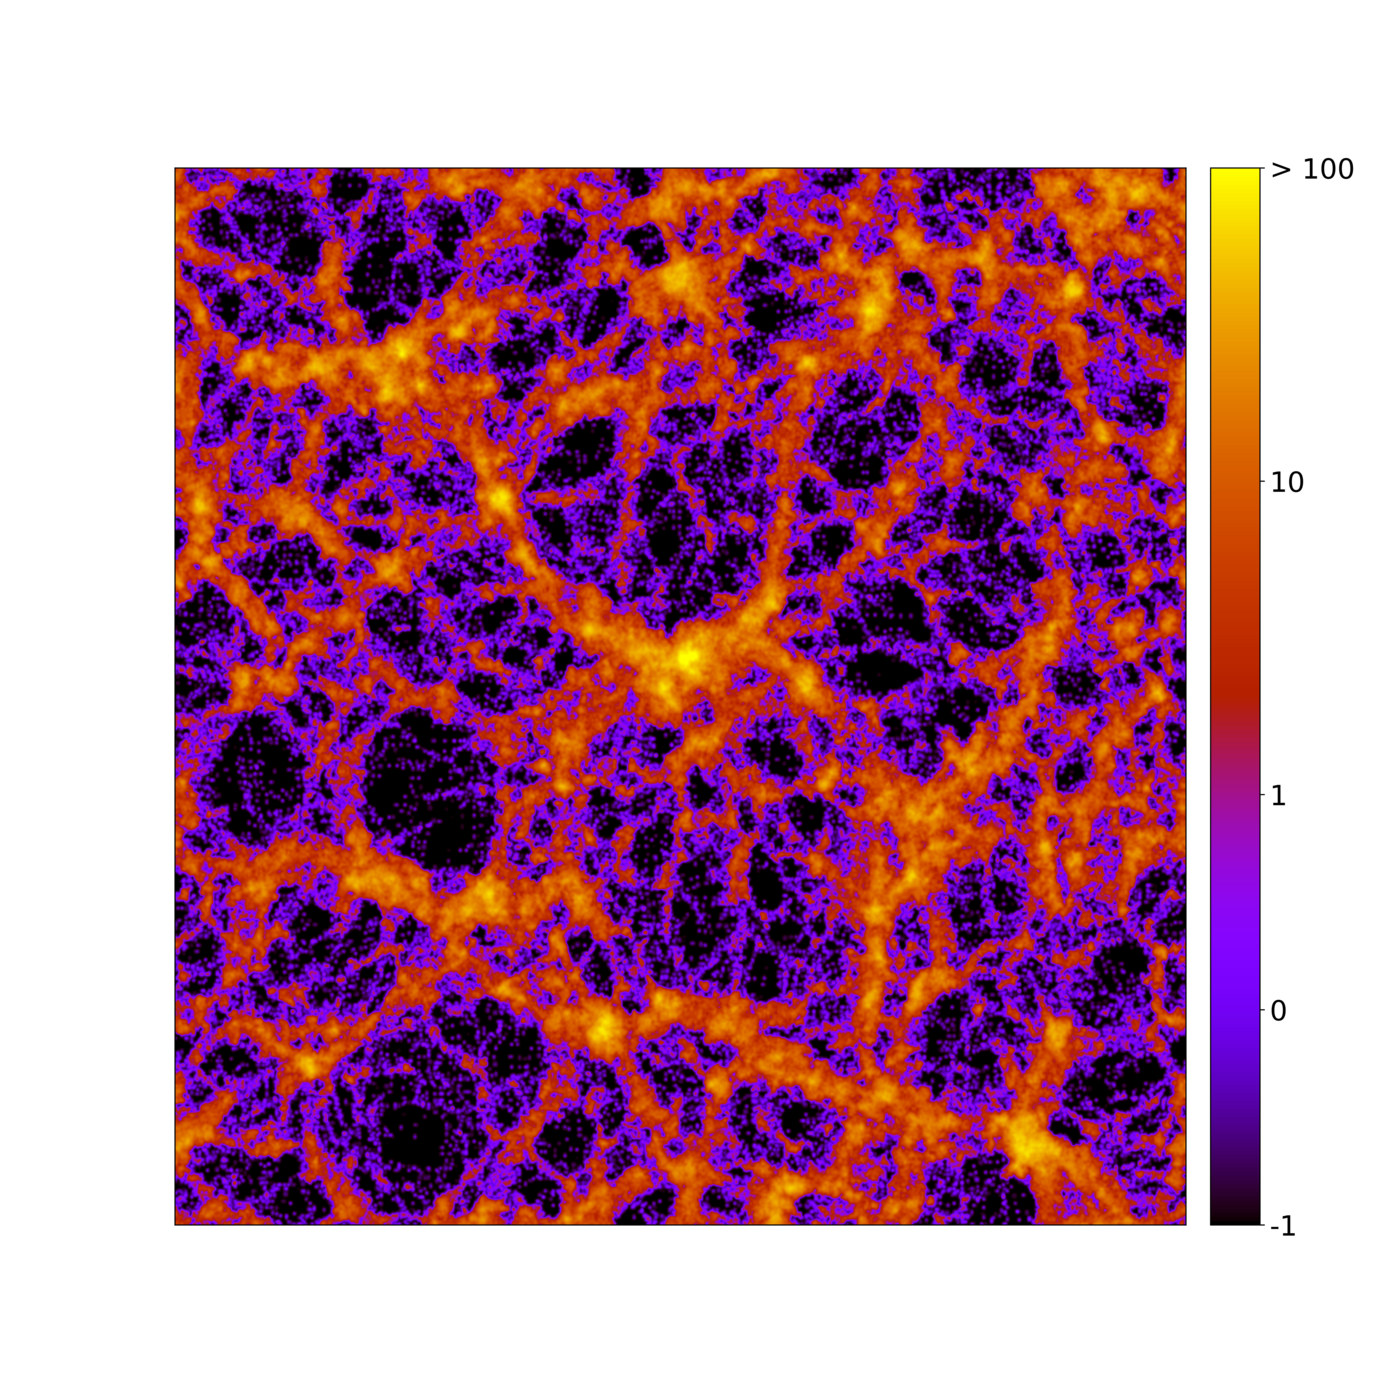
\includegraphics[width=1.0\linewidth]{{simulations_approx/dens/za_dens_512m_1p_1024M_200b_z0.00}.png}
			\caption{Zel'dovich approximation}
		\end{subfigure}
		\begin{subfigure}{0.4\linewidth}
			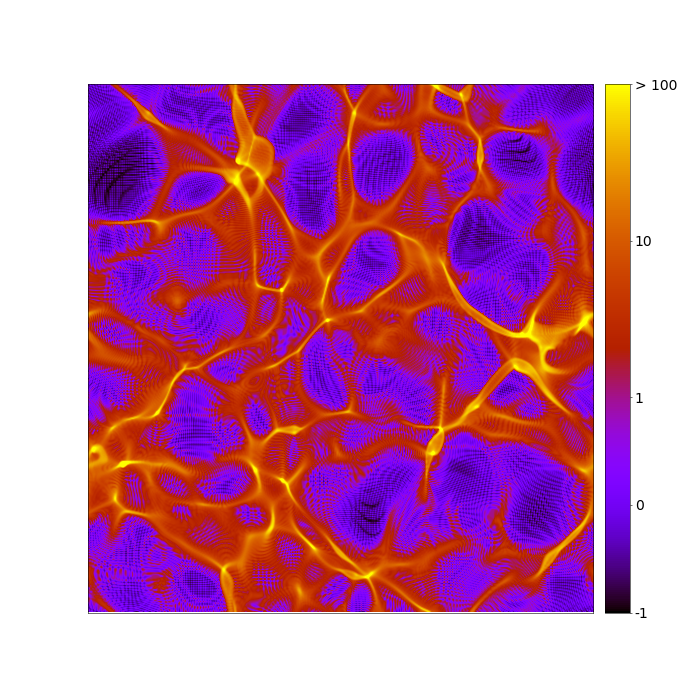
\includegraphics[width=1.0\linewidth]{{simulations_approx/dens/tza_dens_512m_1p_1024M_200b_z0.00}.png}
			\caption{Truncated Zel'dovich approximation}
		\end{subfigure}
		\begin{subfigure}{0.4\linewidth}
			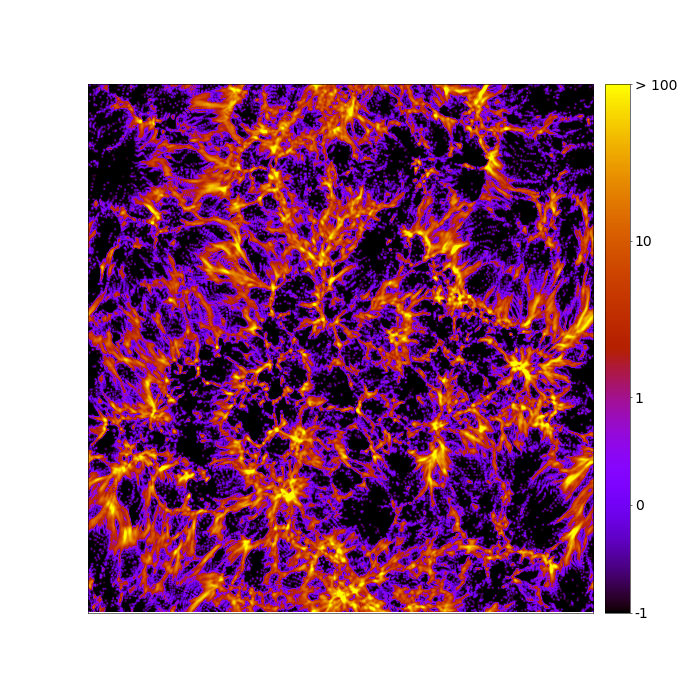
\includegraphics[width=1.0\linewidth]{{simulations_approx/dens/ff_dens_512m_1p_1024M_200b_z0.00}.png}
			\caption{Frozen-flow approximation}
		\end{subfigure}
		\begin{subfigure}{0.4\linewidth}
			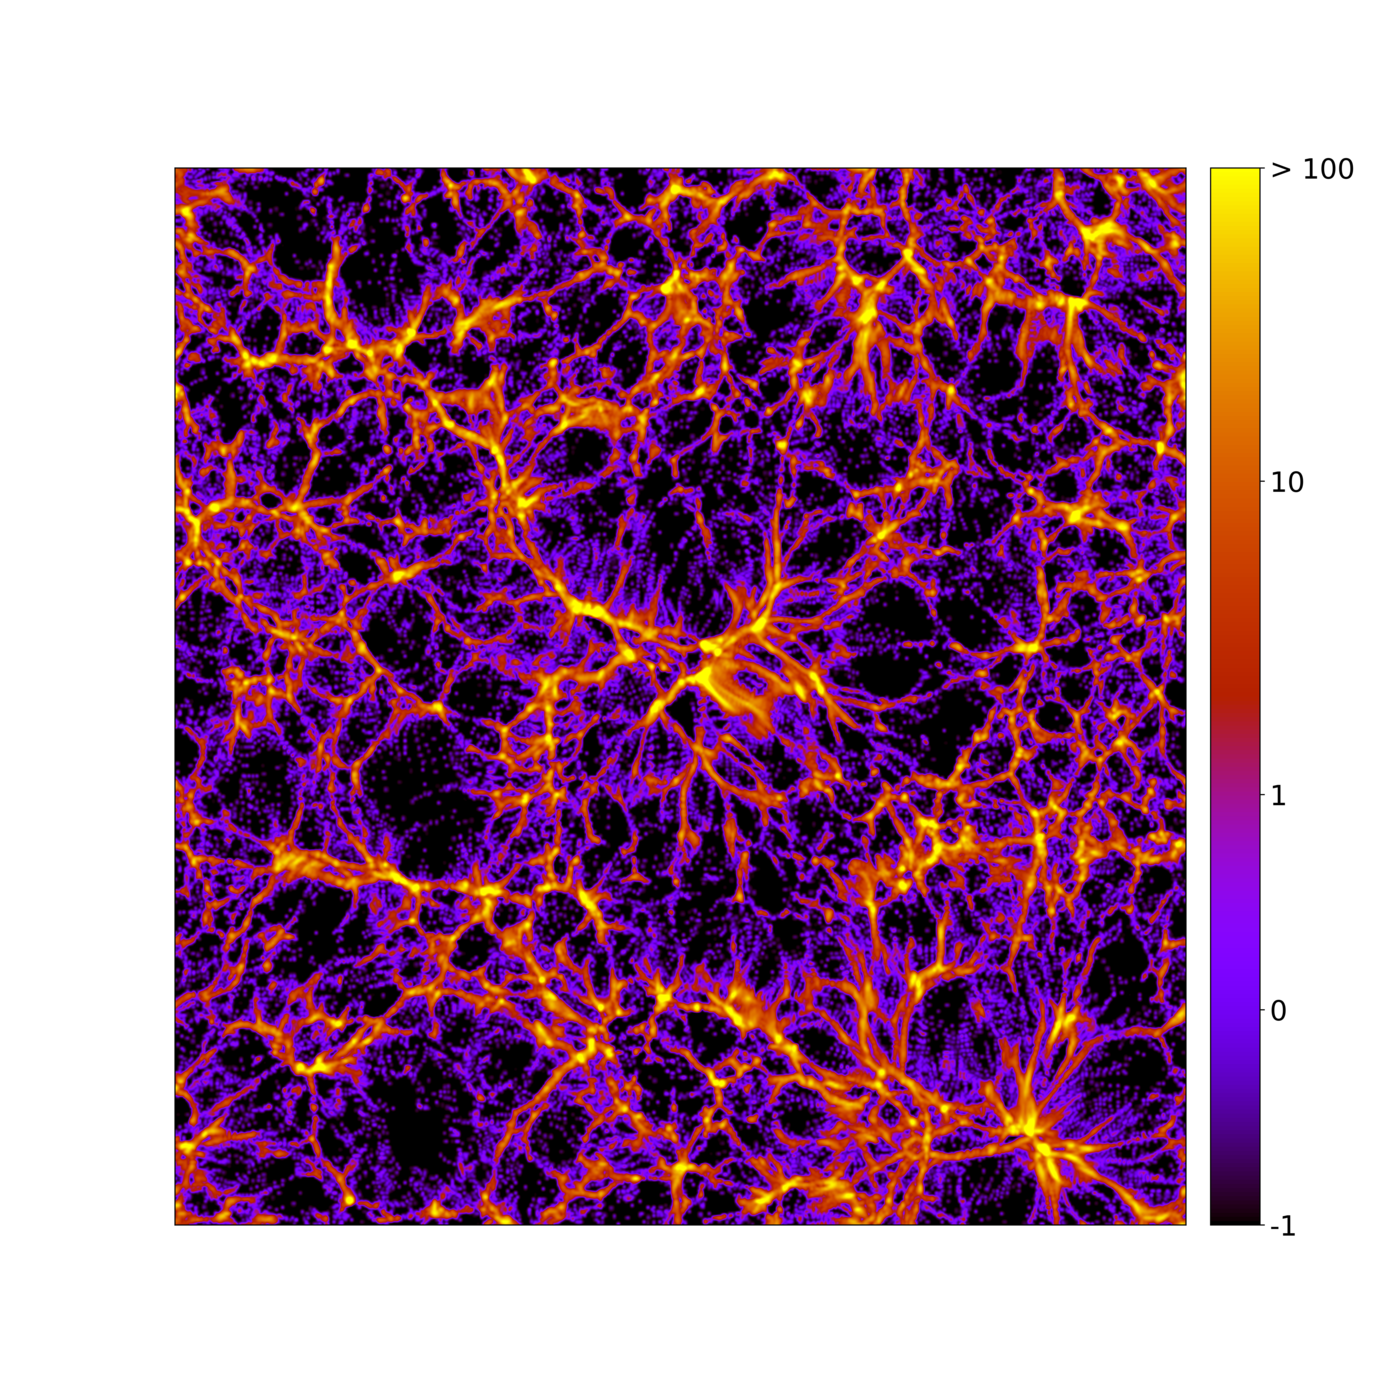
\includegraphics[width=1.0\linewidth]{{simulations_approx/dens/fp_dens_512m_1p_1024M_200b_z0.00}.png}
			\caption{Frozen-potential approximation}
		\end{subfigure}
		\begin{subfigure}{0.4\linewidth}
			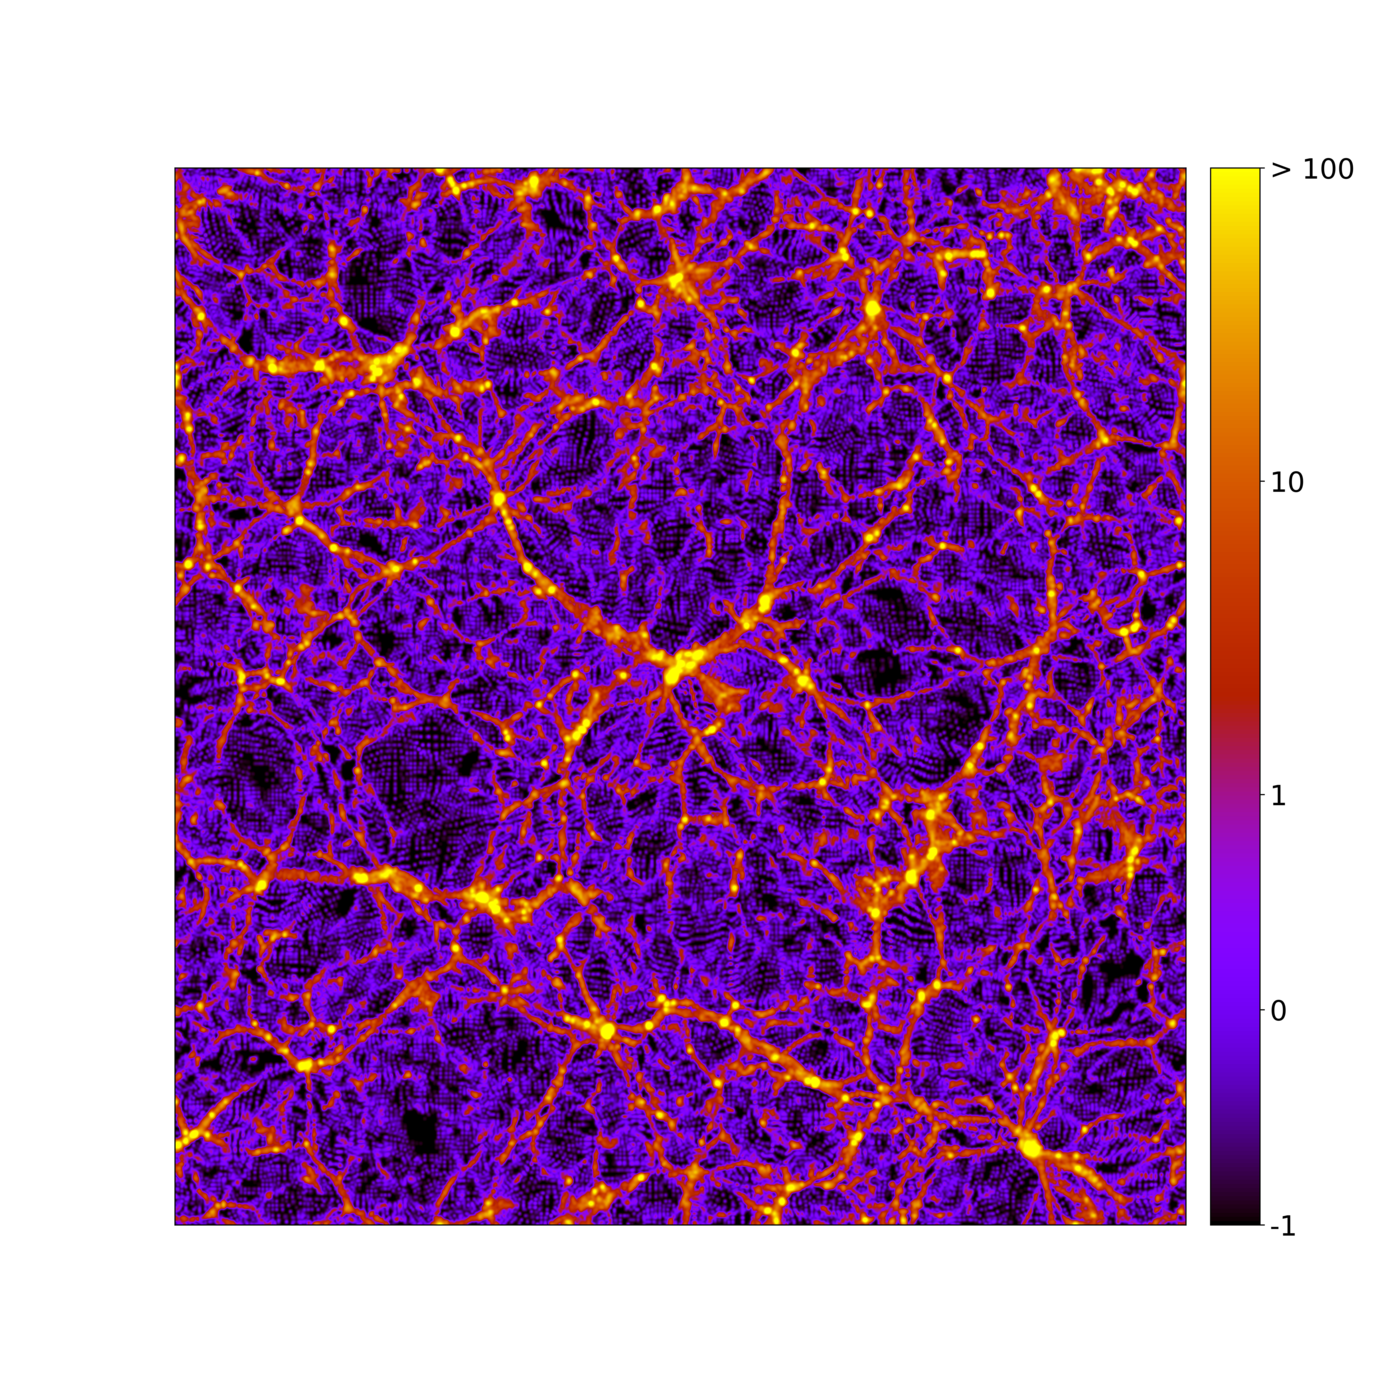
\includegraphics[width=1.0\linewidth]{{simulations_approx/dens/pm_dens_512m_1p_1024M_200b_z0.00}.png}
			\caption{PM simulation}
		\end{subfigure}
	\end{adjustwidth}
		\caption{Projected density field at~redshift $z=0$ for~the~different approximations, all run with~the~same initial conditions. Each slice has a~box-length of~$200~\Mpch$ and~is $1~\Mpch$ thick.}
		\label{fig:slice_dens_all}
\end{figure*}
\floatpagestyle{plain}


\section{Approximation methods in~modified gravity}
Here we remind the~basic chameleon equations we want to~solve numerically. The~non-linear Poisson equation
\eq{
\label{eq:cham_u_cp}
	\Delta\left(\chi/\chi_a\right)= C_\chi(a)\left[1+\delta-\left(\frac{\chi_a}{\chi}\right)^{1-n}\right]\,,
}
where
\eq{
	C_\chi(a)\equiv\frac{3H_0^2\Omega_m}{2\Phiscrz}a^{-3\frac{2-n}{1-n}}=\left(a\mu\Phiscra\right)^{-1}\,,
}
the~linear solution
\eq{
\label{eq:chi_lin_x_cp}
	\chi(\mb x, a) = \chi_a(a)\left(1 + \frac{\Phi_G(\mb x, a)}{\Phiscra(a)} \right)\,.
}
the~linear solution in~$k-$space
\eq
{
\label{eq:chi_lin_k_cp}
	\hat{\chi}(k)=-\frac{\chi_a}{1-n}\frac{m^2}{m^2+k^2}\hat{\delta}(k) = -\frac{\beta\bar\rho_m}{\Mpl}\frac{\hat{\delta}(k)}{k^2+m^2}\,.
}
where the~mass of~the~chameleon field is
\eq{
    \label{eq:chi_m_cp}
	m^2(a)\equiv\frac{1-n}{a\mu\Phiscra}\,,
}
and~the~screened solution inside massive objects
\eq{
	\chi=\frac{\chi_a}{\left(1+\delta\right)^{1/(1-n)}}\,.
	\label{eq:chi_bulk_cp}
}

When applying the~approximation methods to~the~chameleon equations, we have three choices on~how to~arrive at~an~approximate solution:
\begin{enumerate}
\item \label{itm:lin_q} Purely linear prediction in~$(\mb q, a)$-space, solution \eqref{eq:chi_lin_x_cp}

\item \label{itm:lin_k} Purely linear prediction in~$(\mb k, a)$-space, solution \eqref{eq:chi_lin_k_cp}

\item \label{itm:nl_x} Non-linear prediction in~$(\mb x, a)$-space, solution \eqref{eq:cham_u_cp}
\end{enumerate}

Choice \ref{itm:lin_q} means that there is no computational overhead and~we can simply take the~chameleon force to~be $2\beta^2a^{-2}$ of~the~gravitational one. This method clearly overestimates the~chameleon force at~early times when the~chameleon's Compton wavelength is short. This is because the~solution \eqref{eq:chi_lin_x_cp} does not take into account the~non-zero mass of~the~field.

A~better choice is to~use \ref{itm:lin_k} where the~non-zero mass is incorporated. This solution adds relatively little computational overhead over normal gravity -- needing (at~least) one Fourier transform and~also extra storage. The~overdensity $\delta(\mb k, a)$ is either the~linearly evolved one, i.e. $\delta(\mb k, a) = D(a)\delta_0(\mb k)$, or we can compute $\delta$ at~each time-step from the~current positions of~particles. This adds extra computation when assigning the~mass of~particles on~the~grid and~one extra Fourier transform to~get $\delta(\mb k, a)$. 
However, we cannot use \eqref{eq:chi_lin_k_cp} blindly to~get a~solution in~real space as this linear approximation breaks down inside massive objects where we would get a~negative solution. This effect is similar to~usage of~linear evolution for~$\delta$ where we can end up with~regions where $\delta<-1$. We need to~check if the~resulting chameleon field is positive and~fix it where it is not. We use the~screening regime value \eqref{eq:chi_bulk_cp} to~get a~positive solution. We will refer to~this prediction as pseudo-linear since it can address some effects of~the~screening mechanism.

The~most expensive choice is \ref{itm:nl_x} where we must iteratively solve nonlinear equations. Unlike other methods, this one can address the~screening regime inside and~near massive objects but at~the~cost of~the~most computational overhead.

\section{Other approximations}
Approximations described previously are studied numerically in~detail in~the~next chapter. Here we present a~few of~the~other approximations studied in~the~past or used today.

\subsection{Adhesion approximation}
The~adhesion approximation was introduced in~\textcite{1989MNRAS.236..385G}. To~study the~evolution of~density inhomogeneities they used the~model of~non-linear diffusion (Burger's equation), that gives an~approximate description of~the~growth of~structures at~the~advanced non-linear stage of~gravitational instability.

To~overcome problems of~ZA with~shell-crossing they propose a~solution of~``sticking articles.'' Particles move according to~ZA until they ran into one another. Then they move together, with~the~velocity conserving momentum. This model can be described mathematically by inserting the~viscous term into equations of~motion, simulating attractive forces of~gravity
\eq{
	\dddd{\mb u\AAP}{a}=\nu\partpart{^2\mb u}{\mb x^2}\,.
}
The~Burger's equation has an~analytical solution that can be used to~study the~formation of~structures. For~more information regarding the~adhesion approximation see  also \textcite{1990MNRAS.247..260W,1994ApJ...428...28M}.

\subsection{Stable clustering}
It was proposed by \textcite{1974ApJ...189L..51P} that we can study the~behavior of~a~non-linear clustering in~high-density regions by~assuming, that these regions have undergone virialization and~now maintain a~fixed proper density, hence stable clustering. The~correlation function of~such systems would evolve according to
\eq{
	\xi(r,a)\propto1/\bar\rho\propto a^3\,.
}
\textcite{1991ApJ...374L...1H} developed a~model which enabled interpolating between the~linear theory on~large scales and~the~non-linear predictions of~the~stable clustering on~small scales. They showed that the~non-linear two-point correlation function could be parameterized by a~simple function of~the~linear correlation function
\eq{
	\bar\xi_{NL}=f(\bar\xi_{L})\,,
}
where the~functional form of~$f$ can be derived from the~spherical top-hat model without any shell-crossing. For~the~linear regime $\bar\xi_{L}\ll1$, $f(y)=y$, and~for~non-linear $\bar\xi_{L}\gg1$, $f(y)=y^{3/2}$. For~more information regarding the~stable clustering see  also \textcite{1996MNRAS.280L..19P,2003MNRAS.341.1311S}.
\subsection{Lagrangian perturbation theories of~higher-orders}
The~success of~ZA, the~first-order Lagrangian perturbation theory (LPT), has motivated studies of~higher-order corrections \parencite[see e.g.][]{10.1093/mnras/264.2.375,2002PhR...367....1B,2010MNRAS.403.1859J,2014ApJ...788...63S}. In~the~Lagrangian description, the~spatial coordinates are transformed through the~displacement vector $\Psi$ as
\eq{
	\mb x = \mb q + \Psi(a, \mb x)\,.
}
In~LPT, this displacement vector field is expanded in~a~perturbation series in~the~linear growth function $D$ in~Fourier space. Density perturbations $\delta$ are described as a~function of~the~displacement vector through conservation of~mass.\clearpage{}
\clearpage{}\chapter{Simulations with~Approximation Methods}
\label{chpt:app_sims}
In~this chapter we present main results of~our research regarding approximation techniques and~the~possibility to~use these techniques in~studies of~modified gravity. Parts of~this chapter have been published in~\textcite{2020MNRAS.493.2085V}.

We ran our simulations with~the~Planck \LCDM\ cosmology \parencite{planck_cosm}; its parameters are summarized in~\autoref{tab:cosmo_param}. We expect our results to~apply generically to~cosmologies that are not too far from this set of~parameter values.
\begin{table}[!b]
\centering
\begin{tabular}{ l c l }
  \hline \hline
  Hubble constant  [km s$^{-1}$ Mpc$^{-1}$] & $H_0$ & $67.74$ \\
  Baryon density parameter & $\Omega_b$ & $0.0486$ \\
  Matter density parameter & $\Omega_m$ & $0.3089$ \\
  Total density parameter & $\Omega_{tot}$ & $1$ \\
  Scalar spectral index & $n_s$ & $0.9667$ \\
  Fluctuation amplitude at~$8\Mpch$ & $\sigma_8$ & $0.8159$ \\
  \hline \hline
\end{tabular}
\caption{Planck Collaboration cosmological parameters \parencite{planck_cosm} used in~the~simulations.}
\label{tab:cosmo_param}
\end{table}
The non-linear scale \eqref{eq:k_nl} for our chosen power spectrum is $k_{nl}=0.32~\hMpc$. The smoothing scale for TZA is suggested to be in the range from 1 to 1.5 times $k_{nl}$ so we ran the TZA simulations twice, once with $k_G=0.3~\hMpc$ and once with $k_G=0.5~\hMpc$. The results using $k_G=0.5~\hMpc$ proved to be better in terms of predicting the BAO features so we show only those results.

In the plots we use various abbreviations for compactness, while discussing the results of the simulations and the linear and non-linear predictions. These are summarized in \autoref{tab:plots_not}.
\begin{table}[!b]
\centering
\begin{tabular}{ll}
  \hline \hline
  \LCDM\ (lin) & prediction of the linear theory with standard gravity\\
  \LCDM\ (nl) & prediction of the emulator with standard gravity\\
  ZA, TZA, FFA, FPA & simulation run with given approximation and standard gravity\\
  $\chi$ (psl) & simulation run with pseudo-linear prediction of modified gravity\\
  $\chi$ (nl) & simulation run with non-linear solution of modified gravity\\
  \hline \hline
\end{tabular}
\caption{Abbreviations used in the plots.}
\label{tab:plots_not}
\end{table}

In~total, we ran and~analyzed 7117 simulations using different approximations, parameters of~the~simulation volume and~chameleon parameters. Their properties are described in~\autoref{tab:sim_param_ZA_TZA} -- \autoref{tab:cham_param_CHI_nl}.

\begin{landscape}
\begin{table}
    \centering
    \adjustbox{max width=0.45\linewidth, max totalheight=0.9\textheight}{
    \begin{tabular}{ ccccccc }
    \hline \hline
    $L$ & $N_{\rm p}$ & $N_{\rm f}$ & $N_{\rm a}$ & $N$ & $N_t$ & $m$ \\
    \hline
    $100$ & $512^3$ & $512^3$ & $1024^3$ & $1$ & $200$ & $9.4\cdot10^{8}$\\
    $100$ & $512^3$ & $512^3$ & $1024^3$ & $211$ & $100$ & $9.4\cdot10^{8}$\\
    $200$ & $512^3$ & $512^3$ & $1024^3$ & $1$ & $200$ & $7.6\cdot10^{9}$\\
    $200$ & $512^3$ & $512^3$ & $1024^3$ & $2$ & $100$ & $7.6\cdot10^{9}$\\
    $300$ & $512^3$ & $512^3$ & $1024^3$ & $1$ & $200$ & $2.6\cdot10^{10}$\\
    $400$ & $512^3$ & $512^3$ & $1024^3$ & $1$ & $200$ & $6.0\cdot10^{10}$\\
    $500$ & $512^3$ & $512^3$ & $1024^3$ & $1$ & $200$ & $1.2\cdot10^{11}$\\
    $500$ & $512^3$ & $512^3$ & $1024^3$ & $207$ & $100$ & $1.2\cdot10^{11}$\\
    $2000$ & $512^3$ & $512^3$ & $1024^3$ & $20$ & $400$ & $7.6\cdot10^{12}$\\
    $2000$ & $512^3$ & $512^3$ & $1024^3$ & $20$ & $200$ & $7.6\cdot10^{12}$\\
    $2000$ & $512^3$ & $512^3$ & $1024^3$ & $201$ & $100$ & $7.6\cdot10^{12}$\\
    $2000$ & $512^3$ & $512^3$ & $1024^3$ & $20$ & $50$ & $7.6\cdot10^{12}$\\
    $2000$ & $512^3$ & $512^3$ & $1024^3$ & $20$ & $25$ & $7.6\cdot10^{12}$\\
    \hline
    \end{tabular}
    }
    \hspace{2cm}
    \adjustbox{max width=0.45\linewidth, max totalheight=0.9\textheight}{
    \begin{tabular}{ ccccccc }
    \hline \hline
    $L$ & $N_{\rm p}$ & $N_{\rm f}$ & $N_{\rm a}$ & $N$ & $N_t$ & $m$ \\
    \hline
    $100$ & $512^3$ & $512^3$ & $1024^3$ & $1$ & $200$ & $9.4\cdot10^{8}$\\
    $100$ & $512^3$ & $512^3$ & $1024^3$ & $100$ & $100$ & $9.4\cdot10^{8}$\\
    $100$ & $512^3$ & $512^3$ & $1024^3$ & $200$ & $100$ & $9.4\cdot10^{8}$\\
    $200$ & $512^3$ & $512^3$ & $1024^3$ & $1$ & $200$ & $7.6\cdot10^{9}$\\
    $200$ & $512^3$ & $512^3$ & $1024^3$ & $2$ & $100$ & $7.6\cdot10^{9}$\\
    $300$ & $512^3$ & $512^3$ & $1024^3$ & $1$ & $200$ & $2.6\cdot10^{10}$\\
    $400$ & $512^3$ & $512^3$ & $1024^3$ & $1$ & $200$ & $6.0\cdot10^{10}$\\
    $500$ & $512^3$ & $512^3$ & $1024^3$ & $1$ & $200$ & $1.2\cdot10^{11}$\\
    $500$ & $512^3$ & $512^3$ & $1024^3$ & $100$ & $100$ & $1.2\cdot10^{11}$\\
    $500$ & $512^3$ & $512^3$ & $1024^3$ & $201$ & $100$ & $1.2\cdot10^{11}$\\
    $2000$ & $512^3$ & $512^3$ & $1024^3$ & $20$ & $400$ & $7.6\cdot10^{12}$\\
    $2000$ & $512^3$ & $512^3$ & $1024^3$ & $20$ & $400$ & $7.6\cdot10^{12}$\\
    $2000$ & $512^3$ & $512^3$ & $1024^3$ & $20$ & $200$ & $7.6\cdot10^{12}$\\
    $2000$ & $512^3$ & $512^3$ & $1024^3$ & $20$ & $200$ & $7.6\cdot10^{12}$\\
    $2000$ & $512^3$ & $512^3$ & $1024^3$ & $99$ & $100$ & $7.6\cdot10^{12}$\\
    $2000$ & $512^3$ & $512^3$ & $1024^3$ & $201$ & $100$ & $7.6\cdot10^{12}$\\
    $2000$ & $512^3$ & $512^3$ & $1024^3$ & $20$ & $50$ & $7.6\cdot10^{12}$\\
    $2000$ & $512^3$ & $512^3$ & $1024^3$ & $20$ & $50$ & $7.6\cdot10^{12}$\\
    $2000$ & $512^3$ & $512^3$ & $1024^3$ & $20$ & $25$ & $7.6\cdot10^{12}$\\
    $2000$ & $512^3$ & $512^3$ & $1024^3$ & $20$ & $25$ & $7.6\cdot10^{12}$\\
    \hline
    \end{tabular}
    }
    \caption{Parameters of~the~simulations for~ZA (left) and~TZA (right): box size $L$ [$\Mpch$], number of~particles $N_{\rm p}$, number of~force mesh points $\Nf$, number of~power spectrum mesh points $N_{\rm a}$, number of~runs $N$, number of~time-steps $N_t$, and~a~derived parameter particle mass $m$ $[M_\odot]$.}
    \label{tab:sim_param_ZA_TZA}
    \end{table}
    
    
\begin{table}
    \centering
    \adjustbox{max width=0.45\linewidth, max totalheight=0.9\textheight}{
    \begin{tabular}{ ccccccc }
    \hline \hline
    $L$ & $N_{\rm p}$ & $N_{\rm f}$ & $N_{\rm a}$ & $N$ & $N_t$ & $m$ \\
    \hline
    $2000$ & $64^3$ & $64^3$ & $128^3$ & $1$ & $100$ & $3.9\cdot10^{15}$\\
    $2000$ & $256^3$ & $256^3$ & $512^3$ & $99$ & $100$ & $6.0\cdot10^{13}$\\
    $100$ & $512^3$ & $512^3$ & $1024^3$ & $1$ & $200$ & $9.4\cdot10^{8}$\\
    $100$ & $512^3$ & $512^3$ & $1024^3$ & $211$ & $100$ & $9.4\cdot10^{8}$\\
    $200$ & $512^3$ & $512^3$ & $1024^3$ & $1$ & $200$ & $7.6\cdot10^{9}$\\
    $200$ & $512^3$ & $512^3$ & $1024^3$ & $2$ & $100$ & $7.6\cdot10^{9}$\\
    $300$ & $512^3$ & $512^3$ & $1024^3$ & $1$ & $200$ & $2.6\cdot10^{10}$\\
    $400$ & $512^3$ & $512^3$ & $1024^3$ & $1$ & $200$ & $6.0\cdot10^{10}$\\
    $500$ & $512^3$ & $512^3$ & $1024^3$ & $1$ & $200$ & $1.2\cdot10^{11}$\\
    $500$ & $512^3$ & $512^3$ & $1024^3$ & $208$ & $100$ & $1.2\cdot10^{11}$\\
    $2000$ & $512^3$ & $512^3$ & $1024^3$ & $20$ & $400$ & $7.6\cdot10^{12}$\\
    $2000$ & $512^3$ & $512^3$ & $1024^3$ & $20$ & $200$ & $7.6\cdot10^{12}$\\
    $2000$ & $512^3$ & $512^3$ & $1024^3$ & $201$ & $100$ & $7.6\cdot10^{12}$\\
    $2000$ & $512^3$ & $512^3$ & $1024^3$ & $20$ & $50$ & $7.6\cdot10^{12}$\\
    $2000$ & $512^3$ & $512^3$ & $1024^3$ & $19$ & $25$ & $7.6\cdot10^{12}$\\
    \hline
    \end{tabular}
    }
    \hspace{2cm}
    \adjustbox{max width=0.45\linewidth, max totalheight=0.9\textheight}{
    \begin{tabular}{ ccccccc }
    \hline \hline
    $L$ & $N_{\rm p}$ & $N_{\rm f}$ & $N_{\rm a}$ & $N$ & $N_t$ & $m$ \\
    \hline
    $1000$ & $256^3$ & $256^3$ & $512^3$ & $303$ & $100$ & $7.6\cdot10^{12}$\\
    $2000$ & $256^3$ & $256^3$ & $512^3$ & $199$ & $100$ & $6.0\cdot10^{13}$\\
    $100$ & $512^3$ & $512^3$ & $1024^3$ & $1$ & $200$ & $9.4\cdot10^{8}$\\
    $100$ & $512^3$ & $512^3$ & $1024^3$ & $212$ & $100$ & $9.4\cdot10^{8}$\\
    $200$ & $512^3$ & $512^3$ & $1024^3$ & $1$ & $200$ & $7.6\cdot10^{9}$\\
    $200$ & $512^3$ & $512^3$ & $1024^3$ & $2$ & $100$ & $7.6\cdot10^{9}$\\
    $300$ & $512^3$ & $512^3$ & $1024^3$ & $1$ & $200$ & $2.6\cdot10^{10}$\\
    $400$ & $512^3$ & $512^3$ & $1024^3$ & $1$ & $200$ & $6.0\cdot10^{10}$\\
    $500$ & $512^3$ & $512^3$ & $1024^3$ & $1$ & $200$ & $1.2\cdot10^{11}$\\
    $500$ & $512^3$ & $512^3$ & $1024^3$ & $208$ & $100$ & $1.2\cdot10^{11}$\\
    $2000$ & $512^3$ & $512^3$ & $1024^3$ & $20$ & $400$ & $7.6\cdot10^{12}$\\
    $2000$ & $512^3$ & $512^3$ & $1024^3$ & $20$ & $200$ & $7.6\cdot10^{12}$\\
    $2000$ & $512^3$ & $512^3$ & $1024^3$ & $200$ & $100$ & $7.6\cdot10^{12}$\\
    $2000$ & $512^3$ & $512^3$ & $1024^3$ & $20$ & $50$ & $7.6\cdot10^{12}$\\
    $2000$ & $512^3$ & $512^3$ & $1024^3$ & $20$ & $25$ & $7.6\cdot10^{12}$\\
    \hline
    \end{tabular}
    }
    \caption{Parameters of~the~simulations for~FF (left) and~FP (right): box size $L$ [$\Mpch$], number of~particles $N_{\rm p}$, number of~force mesh points $\Nf$, number of~power spectrum mesh points $N_{\rm a}$, number of~runs $N$, number of~time-steps $N_t$, and~a~derived parameter particle mass $m$ $[M_\odot]$.}
    \label{tab:sim_param_FF_FP}
    \end{table}
    
    
     \begin{table}
    \centering
    \adjustbox{max width=0.45\linewidth, max totalheight=0.9\textheight}{
    \begin{tabular}{ ccccccc cc}
    \hline \hline
    $L$ & $N_{\rm p}$ & $N_{\rm f}$ & $N_{\rm a}$ & $N$ & $N_t$ & $m$ & $\Phiscr$ & $n$ \\
    \hline
    $2000$ & $256^3$ & $256^3$ & $512^3$ & $100$ & $100$ & $6.0\cdot10^{13}$ & $1.0\cdot10^{-4}$ & $0.5$ \\
    $2000$ & $256^3$ & $256^3$ & $512^3$ & $96$ & $100$ & $6.0\cdot10^{13}$ & $1.0\cdot10^{-5}$ & $0.7$ \\
    $2000$ & $256^3$ & $256^3$ & $512^3$ & $98$ & $100$ & $6.0\cdot10^{13}$ & $1.0\cdot10^{-6}$ & $0.5$ \\
    $2000$ & $256^3$ & $256^3$ & $512^3$ & $97$ & $100$ & $6.0\cdot10^{13}$ & $1.0\cdot10^{-5}$ & $0.5$ \\
    $2000$ & $256^3$ & $256^3$ & $512^3$ & $99$ & $100$ & $6.0\cdot10^{13}$ & $1.0\cdot10^{-5}$ & $0.1$ \\
    \hline
    \end{tabular}
    }
    \hspace{1cm}
    \adjustbox{max width=0.45\linewidth, max totalheight=0.9\textheight}{
    \begin{tabular}{ ccccccc cc}
    \hline \hline
    $L$ & $N_{\rm p}$ & $N_{\rm f}$ & $N_{\rm a}$ & $N$ & $N_t$ & $m$ & $\Phiscr$ & $n$ \\
    \hline
    $1000$ & $256^3$ & $256^3$ & $512^3$ & $101$ & $100$ & $7.6\cdot10^{12}$ & $1.0\cdot10^{-5}$ & $0.5$ \\
    $2000$ & $256^3$ & $256^3$ & $512^3$ & $100$ & $100$ & $6.0\cdot10^{13}$ & $1.0\cdot10^{-6}$ & $0.5$ \\
    $2000$ & $256^3$ & $256^3$ & $512^3$ & $99$ & $100$ & $6.0\cdot10^{13}$ & $1.0\cdot10^{-5}$ & $0.1$ \\
    $2000$ & $256^3$ & $256^3$ & $512^3$ & $120$ & $100$ & $6.0\cdot10^{13}$ & $1.0\cdot10^{-5}$ & $0.5$ \\
    $2000$ & $256^3$ & $256^3$ & $512^3$ & $100$ & $100$ & $6.0\cdot10^{13}$ & $1.0\cdot10^{-5}$ & $0.7$ \\
    $2000$ & $256^3$ & $256^3$ & $512^3$ & $100$ & $100$ & $6.0\cdot10^{13}$ & $1.0\cdot10^{-4}$ & $0.5$ \\
    $100$ & $512^3$ & $512^3$ & $1024^3$ & $100$ & $100$ & $9.4\cdot10^{8}$ & $1.0\cdot10^{-5}$ & $0.5$ \\
    $500$ & $512^3$ & $512^3$ & $1024^3$ & $100$ & $100$ & $1.2\cdot10^{11}$ & $1.0\cdot10^{-5}$ & $0.5$ \\
    \hline
    \end{tabular}
    }
    \caption{Parameters of~the~pseudo-linear chameleon simulation for~FF (left) and~FP (right): box size $L$ [$\Mpch$], number of~particles $N_{\rm p}$, number of~force mesh points $\Nf$, number of~power spectrum mesh points $N_{\rm a}$, number of~runs $N$, number of~time-steps $N_t$, a~derived parameter particle mass $m$ $[M_\odot]$, screening potential $\Phiscr$, and~the~chameleon power-law exponent $n$.}
    \label{tab:cham_param_CHI_lin}
    \end{table}
    
    
    \begin{table}
    \adjustbox{max width=0.45\linewidth, max totalheight=0.9\textheight}{
    \begin{tabular}{ ccccccc cc}
    \hline \hline
    $L$ & $N_{\rm p}$ & $N_{\rm f}$ & $N_{\rm a}$ & $N$ & $N_t$ & $m$ & $\Phiscr$ & $n$ \\
    \hline
    $2000$ & $256^3$ & $256^3$ & $512^3$ & $100$ & $100$ & $6.0\cdot10^{13}$ & $1.0\cdot10^{-5}$ & $0.5$ \\
    $2000$ & $256^3$ & $256^3$ & $512^3$ & $99$ & $100$ & $6.0\cdot10^{13}$ & $1.0\cdot10^{-5}$ & $0.1$ \\
    $2000$ & $256^3$ & $256^3$ & $512^3$ & $99$ & $100$ & $6.0\cdot10^{13}$ & $1.0\cdot10^{-4}$ & $0.5$ \\
    $2000$ & $256^3$ & $256^3$ & $512^3$ & $100$ & $100$ & $6.0\cdot10^{13}$ & $1.0\cdot10^{-5}$ & $0.7$ \\
    $2000$ & $256^3$ & $256^3$ & $512^3$ & $99$ & $100$ & $6.0\cdot10^{13}$ & $1.0\cdot10^{-6}$ & $0.5$ \\
    \hline
    \end{tabular}
    }
    \hspace{1cm}
    \adjustbox{max width=0.45\linewidth, max totalheight=0.9\textheight}{
    \begin{tabular}{ ccccccc cc}
    \hline \hline
    $L$ & $N_{\rm p}$ & $N_{\rm f}$ & $N_{\rm a}$ & $N$ & $N_t$ & $m$ & $\Phiscr$ & $n$ \\
    \hline
    $1000$ & $256^3$ & $256^3$ & $512^3$ & $77$ & $100$ & $7.6\cdot10^{12}$ & $1.0\cdot10^{-5}$ & $0.5$ \\
    $2000$ & $256^3$ & $256^3$ & $512^3$ & $96$ & $100$ & $6.0\cdot10^{13}$ & $1.0\cdot10^{-6}$ & $0.5$ \\
    $2000$ & $256^3$ & $256^3$ & $512^3$ & $100$ & $100$ & $6.0\cdot10^{13}$ & $1.0\cdot10^{-5}$ & $0.1$ \\
    $2000$ & $256^3$ & $256^3$ & $512^3$ & $102$ & $100$ & $6.0\cdot10^{13}$ & $1.0\cdot10^{-5}$ & $0.5$ \\
    $2000$ & $256^3$ & $256^3$ & $512^3$ & $99$ & $100$ & $6.0\cdot10^{13}$ & $1.0\cdot10^{-5}$ & $0.7$ \\
    $2000$ & $256^3$ & $256^3$ & $512^3$ & $99$ & $100$ & $6.0\cdot10^{13}$ & $1.0\cdot10^{-4}$ & $0.5$ \\
    $100$ & $512^3$ & $512^3$ & $1024^3$ & $100$ & $100$ & $9.4\cdot10^{8}$ & $1.0\cdot10^{-5}$ & $0.5$ \\
    $500$ & $512^3$ & $512^3$ & $1024^3$ & $98$ & $100$ & $1.2\cdot10^{11}$ & $1.0\cdot10^{-5}$ & $0.5$ \\
    \hline
    \end{tabular}
    }
    \caption{Parameters of~the~non-linear chameleon simulation for~FF and~FP: box size $L$ [$\Mpch$], number of~particles $N_{\rm p}$, number of~force mesh points $\Nf$, number of~power spectrum mesh points $N_{\rm a}$, number of~runs $N$, number of~time-steps $N_t$, a~derived parameter particle mass $m$ $[M_\odot]$, screening potential $\Phiscr$, and~the~chameleon power-law exponent $n$.}
    \label{tab:cham_param_CHI_nl}
    \end{table}
     \end{landscape}

\section{Results for~standard gravity}
\subsection{Matter Power Spectrum}
\label{sec:pwr_spec}
The~power spectrum is defined by equation~\eqref{eq:pk}. In~\autoref{fig:pwr_spec_all} we show the~power spectra $P(k)$ at~redshifts $z=0$ and~$z=1.8$ for~the~different approximation schemes. The~gray areas represent variation across different realizations (different simulation runs). We see that on~large (linear) scales all approximations reproduce the~linear theory prediction (note that this is because the~FFA and~FFP results have been compensated for~slower growth, as described below). On~smaller scales, differences between the~approximations become apparent. At~the~higher redshift, the~TZA is still missing a~lot of~power due to~the~initial truncation while ZA sticks close to~the~linear predication. At~$z=0$, the~ZA loses power compared to~the~linear power spectrum on~these scales due to~shell-crossing. In~contrast, FFA and~FPA do much better and~can even partially simulate non-linear clustering.

\begin{figure}[!hbt]
\centering
	\begin{subfigure}{0.9\textwidth}
        \includegraphicscustomlegend{simulations_approx/pwr_spec/pwr_spec_z0.0}
	\end{subfigure}
	\begin{subfigure}{0.9\textwidth}
		\includegraphicscustom{simulations_approx/pwr_spec/pwr_spec_z0.0}
	\end{subfigure}
	\begin{subfigure}{0.9\textwidth}
		\includegraphicscustom{simulations_approx/pwr_spec/pwr_spec_z1.8}
	\end{subfigure}
	\caption{Matter power spectrum $P(k)$ at~redshifts $z=0$ (top) and~$z=1.8$ (bottom) for~different approximation schemes. Grey areas represent variations across different runs. At~$z=1.8$, the~TZA is much below the~linear prediction due to~the~initial truncation whereas ZA stick close to~the~linear prediction. At~$z=0$, due to~shell-crossing, ZA filters the~power at~higher $k$, falling below the~linear power spectrum, whereas FFA and~FPA retain some features of~the~full non-linear clustering.}
    \label{fig:pwr_spec_all}
\end{figure}

\subsubsection{Comparison with~linear theory}
The~relative differences between power spectra and~the~linear predictions at~different redshifts are plotted in~\autoref{fig:pwr_spec_diff}. By the~linear prediction, in~this case, is meant the~initial power spectrum of~the~realization linearly evolved to~the~given epoch. The~error bars once again represent variation across different realizations but individual differences are computed from the~same realization of~the~power spectrum.
\begin{figure*}[!hbt]
	\begin{adjustwidth}{-1cm}{-1cm}
	\centering
		\begin{subfigure}{1.0\linewidth}
			\includegraphicscustomlegend{simulations_approx/pwr_spec/pwr_spec_diff_init_ZA}
		\end{subfigure}
		\begin{subfigure}{0.5\linewidth}
			\includegraphicscustom{simulations_approx/pwr_spec/pwr_spec_diff_emu}	
			\caption{\LCDM\ (nl)}	
		\end{subfigure}
		\begin{subfigure}{0.5\linewidth}
			\includegraphicscustom{simulations_approx/pwr_spec/pwr_spec_diff_init_ZA}
			\caption{Zel'dovich approximation}
		\end{subfigure}
		\begin{subfigure}{0.5\linewidth}
			\includegraphicscustom{simulations_approx/pwr_spec/pwr_spec_diff_init_TZA}
			\caption{Truncated Zel'dovich approximation}
		\end{subfigure}
		\begin{subfigure}{0.5\linewidth}
			\includegraphicscustom{simulations_approx/pwr_spec/pwr_spec_diff_init_FF}
			\caption{Frozen-flow approximation}
		\end{subfigure}
		\begin{subfigure}{0.5\linewidth}
			\includegraphicscustom{simulations_approx/pwr_spec/pwr_spec_diff_init_FP}
			\caption{Frozen-potential approximation}
		\end{subfigure}
	\end{adjustwidth}
	\caption{Relative differences between power spectra of~approximations and~the~linear prediction at~different redshifts. ZA predicts power spectra at~large scales very well but fails on~small scales at~later times. FFA and~FPA do not have this problem at~small scales but the~power spectrum grows more slowly across all scales. The~(CosmicEmu) non-linear power spectrum is shown in~the~upper panel for~comparison.}
	\label{fig:pwr_spec_diff}
\end{figure*}

The~upper panel shows the~non-linear power spectrum $P(k)$ generated by the~CosmicEmu emulator \parencite{Heitmann:2015xma} for~comparison purposes. The~emulator predictions involve interpolations across results from a~finite number of~high-resolution simulations run with~different cosmological parameters; the~results are accurate at~the~level of~a~few percent.

As expected, the~ZA predicts power spectra at~large scales very well but fails on~small scales at~later times. In~the~case of~FFA and~FPA, the~power spectrum growth is slower than linear theory predicts but, unlike ZA, this behavior is across all scales and~there is significantly less suppression of~power on~smaller scales. 
\subsection{Effective Redshift}
\label{sec:z_eff}
The~power spectrum growth is slower than the~linear prediction in~the~case of~FFA or FPA. For~FFA, this can be understood from the~equation of~motion \eqref{eq:FFA}. As the~particles approach the~minimum of~the~gravitational well, their velocities decrease as the~gradient of~the~potential drops. In~these approximations, as the~velocity potential is constant in~time, there is no change in~slope as more and~more particles arrive into the~gravitational well, which is certainly not realistic. (If possible, the~resulting artifacts should be corrected when using these approximations.)

For~FPA, the~reason for~the~suppression is very similar, although not as significant. Particles are not moving without any memory of~their previous positions as in~the~case of~FFA. They do not stop at~the~bottom of~the~well but rather oscillate around it. However, equation \eqref{eq:FPA} still drives them toward the~velocities of~FFA and~they slow down inside gravitational wells.

Note that this effect of~slower growth due to~a~decreasing gradient of~the~velocity potential is not bound to~some particular scale -- it occurs both in~shallow large wells as well as in~deep and~more concentrated wells. Consequently, it can be compensated via a~correction factor. A~similar situation occurs in~particle-mesh codes when the~number of~time-steps is restricted because the~assumption of~constancy in~velocity and~force (the~``drift'' and~``kick'' terms in~a~standard integrator) fails to~hold. In~approximate particle-mesh codes, this error may be compensated by employing a~ZA-motivated correction~(\cite{Ref:Feng}) in~the~time-stepping. The~same technique could be applied here by combining the~approximations in~a~suitable way or, as we do, by simply calibrating against linear theory, which yields the~same result.

Additionally, the~dynamical approximations in~FFA and~FPA can lead to~artificial non-linear enhancement of~the~growth at~later times on~small scales within deep wells. It takes more time to~get into a~local gravitational well than in~standard \nbody\ but once the~particles are there, they may form stable cores as they simply move towards the~local potential minimum. On~these small scales, the~approximations are not valid in~any case, so this point is mostly academic.

As discussed above, the~suppression of~linear growth in~FFA and~FPA can be viewed as a~modified growth function and~we can introduce a~simple rescaling via an~effective redshift $z\eff$ so that the~power spectrum on~large linear scales matches the~linear prediction
\eq{
	\langle P(k, z\eff) \rangle = \langle P\lin(k, z)\rangle\,,
}
where we are averaging over ``large scales''. In~our simulations, this means we are fitting the~linear power spectrum in~the~range from the~minimum available wave-number $k_\text{\tiny min}=2\pi/L$ to~half a~decade $k=\sqrt{10}k_\text{\tiny min}$.

In~the~rest of~the~paper when we are comparing our results with~a~prediction of~the~linear or non-linear theory, we use this effective time instead of~the~simulation time unless stated otherwise.

In~\autoref{fig:D_eff_Pk}, we compare the~effective growth function with~the~linear growth function of~\LCDM. For~ZA and~TZA there is almost no suppression as we are comparing large scales. However, at~later times (or if we had used smaller scales) we would see an~exponential suppression as described in~\cite{Bharadwaj_1996}. For~FFA and~FPA we have an~almost linear dependence of~$D\eff$ on~$a$, for~FFA with~a~slope of~approximately $8\%$ and~for~FPA with~the~slope being approximately $6\%$.
\begin{figure}[!bt]
  \centering
    \begin{subfigure}{0.9\textwidth}
        \includegraphicscustomlegend{simulations_approx/z_eff/D_eff_Pk}
	\end{subfigure}
	\begin{subfigure}{0.9\textwidth}
        \includegraphicscustom{simulations_approx/z_eff/D_eff_Pk}
	\end{subfigure}
  \caption{Effective growth factor $D\eff$ for~different approximation schemes based on~the~ratio of~power spectrum on~large scales compared to~the~linear prediction.}
  \label{fig:D_eff_Pk}
\end{figure}

In~\autoref{fig:timestep} we study the~dependence of~$D\eff$ on~the~number of~time-steps. A~larger number of~time-steps improves $D\eff$ for~FPA but, as expected, cannot eliminate the~effect. In~the~case of~FFA, $D\eff$ actually decreases with~an~increase in~the~number of~time-steps. In~this case, for~a~smaller number of~time-steps, particles do not evolve exactly along characteristic curves of~the~(initial) potential, and~the~deceleration is suppressed.
\begin{figure}[!bt]
  \centering
    \begin{subfigure}{0.9\textwidth}
        \includegraphicscustomlegend{simulations_approx/z_eff/timesteps}
	\end{subfigure}
	\begin{subfigure}{0.9\textwidth}
        \includegraphicscustom{simulations_approx/z_eff/timesteps}
	\end{subfigure}
  \caption{Effective growth factor $D\eff$ at~$z=0$ for~FFA and~FPA as a~function of~the~number of~time-steps.}
  \label{fig:timestep}
\end{figure}

After the~linear theory compensation via the~effective time, all approximations match the~linear prediction on~large scales (by definition), however, on~smaller scales, there are considerable differences. In~the~case of~ZA (and~TZA) at~early times there is an~enhancement of~power above linear theory, but at~later times, the~lack of~the~ability to~follow small-scale structure (``diffusion'' at~caustics) causes a~suppression of~power that continues to~leak to~larger scales. For~FFA and~FPA, however, the~behavior is quite different. At~early times particles on~the~smallest scales are almost in~the~minimum of~the~local gravitational potential (and~consequently at~the~minimum of~the~velocity potential) and~do not evolve much. This effect is weaker for~FPA where particles have inertia and~are not overdamped. At~later times more and~more particles end up in~these (constant-in-time) gravitational wells and~we observe (partial) non-linear gravitational clustering.
 
\subsection{Correlation Function}
\label{sec:corr}
The~two-point correlation function is defined by the~equation \eqref{eq:corr}. We computed the~correlation function as an~inverse Fourier transformation of~\eqref{eq:pk_xi} as
\eq{
\label{eq:bao}
\xi(r)=\left\langle \delta(\mb x)\delta(\mb{x+r})\right\rangle=\int\frac{\dd^3\mb k}{(2\pi)^3}P(k)e^{i\mb{k\cdot r}}\,.
}
We computed the~correlation function $\xi(r)$ for~different approximation schemes at~different redshifts directly from the~measured matter power spectrum $P(k)$ using equation \eqref{eq:bao}. In~\autoref{fig:corr_func}, we display an~example of~the~correlation function at~redshift $z=0.5$. All approximations agree reasonably with~the~full non-linear predictions of~the~emulator for~the~location of~the~BAO peak and~its width.
\begin{figure}[bt]
\centering
	\begin{subfigure}{0.9\textwidth}
        \includegraphicscustomlegend{simulations_approx/corr_func/corr_func_r2_z_z_eff}
	\end{subfigure}
	\begin{subfigure}{0.9\textwidth}
		\centering
		\includegraphicscustom{simulations_approx/corr_func//corr_func_r2_z_z_eff}
	\end{subfigure}
	\caption{Two-point correlation function for~different approximation schemes at~$z=0.5$}.
	\label{fig:corr_func}
\end{figure}

Individual features of~the~BAO peak -- location $r_0$, amplitude $A$ and~width $\sigma$ -- are obtained by fitting a~Gaussian to~$r^2\xi(r)$ around the~BAO peak
\eq{
\xi_G(r)=A\cdot e^{-(r-r_0)^2/2\sigma^2}
}
In~\autoref{fig:corr_peak}, we show these features of~the~BAO peak relative to~the~non-linear predictions of~the~emulator as a~function of~time. All approximations can predict the~location of~the~peak with~1\% accuracy. In~predicting the~shape of~the~peak, however, they do worse -- all approximations deviate in~predictions for~the~peak width and~amplitude. Note that which approximation does best (compared to~the~others) for~a~given quantity is a~function of~redshift.


\begin{figure}[tbp]
\newcommand{\corrwidth}{0.70}
\centering
	\begin{subfigure}{\corrwidth\textwidth}
        \includegraphicscustomlegend{simulations_approx/corr_func/corr_peak_loc_z_eff}
	\end{subfigure}
	\begin{subfigure}{\corrwidth\textwidth}
		\centering
		\includegraphicscustom{simulations_approx/corr_func//corr_peak_loc_z_eff}
		\caption{Location}
	\end{subfigure}
	\begin{subfigure}{\corrwidth\textwidth}
		\centering
		\includegraphicscustom{simulations_approx/corr_func//corr_peak_amp_z_eff}
		\caption{Amplitude}
	\end{subfigure}
	\begin{subfigure}{\corrwidth\textwidth}
		\centering
		\includegraphicscustom{simulations_approx/corr_func//corr_peak_width_z_eff}
		\caption{Width}
	\end{subfigure}
	\caption{Location, amplitude and~width of~the~BAO peak (relative to~the~non-linear prediction) as a~function of~the~redshift.}
	\label{fig:corr_peak}
\end{figure}

\subsection{Halo mass function}
We computed the~halo mass function \eqref{eq:hmf} from the~amplitude of~density fluctuations for~all approximation schemes. Four our simple analysis we just use the~fitting formula \eqref{eq:hmf_jenkins} instead of~implementing the~full friend-of-friend algorithm.

The~comparison of~approximations in~mass range $(10^{11}-10^{15}M_\odot)$, is shown in~\autoref{fig:hmf_diff_z}. We see that TZA for~higher redshifts is completely wrong as its missing a~lot of~power on~these scales. At~higher redshifts, this gets better as the~TZA gets more power on~these scales without so much shell-crossing as ZA. We see that for~$z=0$ TZA gives results closer to~the~linear prediction than ZA.
\begin{figure*}[p]
	\thisfloatpagestyle{empty}
	\centering
	\begin{subfigure}{1.0\textwidth}
		\includegraphicscustomlegend{simulations_approx/hmf/z0.0_b100_M1024_hmf_z_z_eff}
	\end{subfigure}
	\begin{subfigure}{0.5\textwidth}
		\includegraphicscustom{simulations_approx/hmf/z3.9_b100_M1024_hmf_z_z_eff}
		\caption{$z=\zone$}
	\end{subfigure}
	\begin{subfigure}{0.5\textwidth}
		\includegraphicscustom{simulations_approx/hmf/z1.8_b100_M1024_hmf_z_z_eff}
		\caption{$z=\ztwo$}
	\end{subfigure}
	\begin{subfigure}{0.5\textwidth}
		\includegraphicscustom{simulations_approx/hmf/z0.5_b100_M1024_hmf_z_z_eff}
		\caption{$z=\zthree$}
	\end{subfigure}
	\begin{subfigure}{0.5\textwidth}
		\includegraphicscustom{simulations_approx/hmf/z0.0_b100_M1024_hmf_z_z_eff}
		\caption{$z=\zfour$}
	\end{subfigure}
	\begin{subfigure}{0.5\textwidth}
		\includegraphicscustom{simulations_approx/hmf/diff_z3.9_b100_M1024_hmf_z_z_eff}
		\caption{$z=\zone$}
	\end{subfigure}
	\begin{subfigure}{0.5\textwidth}
		\includegraphicscustom{simulations_approx/hmf/diff_z1.8_b100_M1024_hmf_z_z_eff}
		\caption{$z=\ztwo$}
	\end{subfigure}
	\begin{subfigure}{0.5\textwidth}
		\includegraphicscustom{simulations_approx/hmf/diff_z0.5_b100_M1024_hmf_z_z_eff}
		\caption{$z=\zthree$}
	\end{subfigure}
	\begin{subfigure}{0.5\textwidth}
		\includegraphicscustom{simulations_approx/hmf/diff_z0.0_b100_M1024_hmf_z_z_eff}
		\caption{$z=\zfour$}
	\end{subfigure}
	\caption{Halo mass function for~different approximation schemes at~different redshifts. Top four (a -- d) are absolute functions while four bottom ones (e -- h) represents HMFs relative to~non-linear prediction of~\LCDM.}
	\label{fig:hmf_diff_z}
\end{figure*}
\floatpagestyle{plain}

Also in~\autoref{fig:hmf_diff_z} we show the~halo mass function in~more detail, mainly as a~relative difference between prediction of~approximation schemes and~prediction of~the~non-linear theory. We see that approximation schemes generally predicts less massive halos $(M\gtrsim10^{12}M_\odot)$ and~more light halos $(M\lesssim10^{12}M_\odot)$. We see that simple PM simulations get results close to~the~non-linear prediction, except at~higher redshift. 
\section{Results for~modified gravity}
\newcommand{\chileft}{\hspace*{-1cm}}
In~this section, we apply the~approximate techniques to~chameleon gravity. Parameters of~all run and~analyzed simulations are described in~\autoref{tab:cham_param_CHI_lin} and~\autoref{tab:cham_param_CHI_nl}. We focused on~issues closely related to~the~scale where the~chameleon field starts to~affect the~matter distribution. We first wish to~study the~effects of~varying the~simulation resolution on~the~power spectrum. Because the~screening mechanism is directly related to~the~depth of~the~gravitational wells, and~with~lower spatial resolution, these wells are smeared, the~role of~the~resolution also needs to~be understood. For~this analysis, we chose the~FPA as this approximation is closest in~spirit to~\nbodysim s.

Following this, we compare the~results of~chameleon gravity directly against the~FPA and~FFA simulations. 
We will study both $k-$space effects (power spectrum) and~real-space effects (BAO peak in~the~correlation function). For~chameleon gravity we ran all simulations twice -- once solving the~non-linear Poisson equation \eqref{eq:cham_u_cp} using the~multigrid solver, and~the~second using the~pseudo-linear prediction for~the~chameleon in~$k-$space given by \eqref{eq:chi_lin_k_cp} corrected by \eqref{eq:chi_bulk_cp}.

\subsection{Effect of~simulation resolution}
In~order to~study the~effects of~the~simulation resolution, we define this resolution via the~Nyquist wave-number $\knq$
\eq{
\knq=\frac{\pi N_f}{L}\,.
}
We wish to~study two things in~particular. The~first is the~minimum resolution needed to~explore some particular scale, i.e., whether non-linear effects on~smaller scales can affect larger scales. The~second is to~study the~validity range of~the~pseudo-linear approximation of~the~chameleon field. We want to~investigate on~which scale this approximation breaks down and~cannot be used even for~generating approximate results.

In~\autoref{fig:chi_res}, we see several chameleon simulations $(n=0.5,\ \Phiscr=10^{-5})$ with~different resolutions. We compared the~resulting power spectra directly with~FPA simulations with~the~same parameters (box size, number of~particles, etc.). There are four sets of~simulations with~different resolutions (Nyquist frequencies), each one with~a~pseudo-linear prediction for~the~chameleon field and~a~non-linear result from the~multigrid solver.

\begin{figure}[bt]
	\centering
	  \begin{subfigure}{0.85\textwidth}
		  \includegraphicscustomlegend{simulations_approx/chi/chi_resolution_eff}
	  \end{subfigure}
	  \begin{subfigure}{0.85\textwidth}
		  \includegraphicscustom{simulations_approx/chi/chi_resolution_eff}
	  \end{subfigure}
	\caption{Ratio of~the~power spectrum of~chameleon gravity to~FPA with~different resolutions of~simulations. All simulations have $n=0.5,\ \Phiscr=10^{-5}$. Dotted lines show the~pseudo-linear prediction of~the~chameleon field whereas solid lines show results for~the~full non-linear multigrid solver for~the~chameleon field. Dashed vertical lines show locations of~corresponding Nyquist frequencies.}
	\label{fig:chi_res}
\end{figure}
For~lower resolutions $(\knq = 0.4~\hMpc$ and~$\knq = 0.8~\hMpc)$, the~pseudo-linear theory predicts a~higher amplitude of~the~power spectrum as it underestimates the~screening effect on~smaller scales. However, with~higher resolution (and~the~ability to~see deeper gravitational wells) this pseudo-linear prediction starts to~overestimate the~screening and~suppress the~power spectrum sooner than in~the~non-linear solver. It is because the~correction to~the~solution \eqref{eq:chi_lin_k_cp} suppresses the~chameleon force completely -- not only inside massive objects but near those as well. The~non-linear solution predicts suppressed forces nearby these massive objects but not completely. The~exact scale when this happens is dependent on~the~screening potential -- lower $\Phiscr$ means we need a~finer resolution to~see deep gravitational wells where the~chameleon is in~the~screening regime. For~the~choice of~the~screening potential as in~\autoref{fig:chi_res} $(\Phiscr=10^{-5})$ this crossover where we cannot use the~linear prediction happens at~$k\sim2~\hMpc$. However, as FPA cannot fully resolve non-linear features on~scales $k\gtrsim1~\hMpc$  we cannot take this scale exactly.

We can also see that even with~higher resolution the~power spectra on~large and~medium scales remain the~same. This may suggest that the~non-linear effects due to~the~coupling of~different wave-numbers are small. However, as these results are coming from a~quasi-linear approximation we should be cautious about such a~statement. We will further explore this resolution effects of~the~chameleon gravity using full \nbodysim s in~the~future.
\subsection{Matter power spectrum}
We now turn to~results for~the~matter power spectrum; \autoref{fig:pwr_spec_chi_fp} shows power spectra for~different chameleon parameters for~modified gravity simulations with~FFA and~FPA.
\begin{figure*}[bt]
	\begin{adjustwidth}{-1cm}{-1cm}
	\centering
		\begin{subfigure}{1.2\textwidth}
			\includegraphicscustomlegend{simulations_approx/chi/fp_pwr_spec}
		\end{subfigure}
		\begin{subfigure}{0.5\textwidth}
			\includegraphicscustom{simulations_approx/chi/fp_pwr_spec}
		\end{subfigure}
		\begin{subfigure}{0.5\textwidth}
			\includegraphicscustom{simulations_approx/chi/ff_pwr_spec}
		\end{subfigure}
		\begin{subfigure}{0.5\textwidth}
			\includegraphicscustom{simulations_approx/chi/fp_pwr_spec_ratio_nl}
		\end{subfigure}
		\begin{subfigure}{0.5\textwidth}
			\includegraphicscustom{simulations_approx/chi/ff_pwr_spec_ratio_nl}
		\end{subfigure}
	\end{adjustwidth}
    \caption{Matter power spectrum $P(k)$ at~redshift $z=0$ for~different chameleon parameters. On~the~left are results using FPA whereas on~the~right results using FFA. Grey areas represent variations across different runs. Higher screening potential leads to~greater enhancement of~the~power spectrum due to~the~fifth force.}
    \label{fig:pwr_spec_chi_fp}
\end{figure*}

The~FFA predicts an~increased enhancement of~the~power spectrum compared to~the~FPA, unlike the~corresponding situation for~$\Lambda$CDM. This can be understood from how dynamics are treated within the~FFA. In~the~case of~standard gravity, the~velocity of~a~particle decreases steadily as it approaches a~minimum of~the~gravitational potential. In~the~case of~chameleon gravity, however, once the~particle is close enough to~the~potential minimum such that the~screening effect kicks in, the~fifth force is abruptly cut off and~the~particle stops at~the~potential minimum. In~the~case of~FPA, the~particles retain their velocities inside the~screened regions and~the~clustering effect, therefore, is not as strong.

In~\autoref{fig:CHI_FP_diff}, we compare simulations with~different chameleon parameters directly with~FPA and~FFA. For~the~values of~the~chosen screening potential $(\Phiscr=10^{-6}, 10^{-5}, 10^{-4})$ and~a~given resolution, the~pseudo-linear prediction slightly underestimates the~screening effect. The~dependence of~the~enhancement of~the~power spectrum on~chameleon parameters is according to~our expectations. A~lower value of~the~screening potential leads to~a~shorter Compton wavelength and~greater effect of~screening and~therefore lower enhancement. The~lower value of~the~chameleon power-law exponent leads to~a~longer Compton wavelength and~higher screening potential $\Phiscra$ and~therefore greater enhancement. We also again see that FFA predicts greater enhancement than FPA.

\begin{figure*}[tb]
  \centering
  \chileft
	\begin{subfigure}{1.2\textwidth}
        \includegraphicscustomlegend{simulations_approx/chi/chi_pwr_diff_256m_1p_512M_2000b}
	\end{subfigure}
	\begin{subfigure}{0.5\textwidth}
		\includegraphicscustom{simulations_approx/chi/chi_pwr_diff_256m_1p_512M_2000b}
	\end{subfigure}
	\begin{subfigure}{0.5\textwidth}
		\includegraphicscustom{simulations_approx/chi/chi_ff_pwr_diff_256m_1p_512M_2000b}
	\end{subfigure}
  \caption{Ratio of~the~power spectrum of~chameleon gravity to~FPA (left) and~FFA (right) with~different chameleon parameters. Dotted lines show the~pseudo-linear prediction of~the~chameleon field whereas solid lines show results for~the~full non-linear multigrid solver.}
  \label{fig:CHI_FP_diff}
\end{figure*}

In~\autoref{fig:CHI_FP_diff_lin_ratio} we show the~ratio of~the~power spectrum using the~full non-linear solver of~the~chameleon field to~results using pseudo-linear predictions. The~enhancement of~the~pseudo-linear prediction on~scales $k\sim0.1~\Mpch$ is at~percent level, while again somewhat stronger for~FFA.

\begin{figure*}[!tb]
  \centering
	\begin{subfigure}{1.2\textwidth}
		\chileft
        \includegraphicscustomlegend{simulations_approx/chi/chi_pwr_diff_256m_1p_512M_2000b_lin_ratio}
	\end{subfigure}
	\begin{subfigure}{0.5\textwidth}
		\includegraphicscustom{simulations_approx/chi/chi_pwr_diff_256m_1p_512M_2000b_lin_ratio}
	\end{subfigure}
	\begin{subfigure}{0.5\textwidth}
		\includegraphicscustom{simulations_approx/chi/chi_ff_pwr_diff_256m_1p_512M_2000b_lin_ratio}
	\end{subfigure}
  \caption{Ratio of~the~power spectrum of~chameleon gravity to~pseudo-linear prediction using FPA (left) and~FFA (right) with~different chameleon parameters.}
  \label{fig:CHI_FP_diff_lin_ratio}
\end{figure*}

In~\autoref{fig:chi_pwr_diff_map}, we compare chameleon gravity to~the~FPA through the~ratio of~their power spectra for~one set of~chameleon parameters $(n=0.5,\ \Phiscr=10^{-5})$ as a~function of~time and~scale. Here we can see a~comparison of~a~non-linear prediction as well as a~comparison with~the~chameleon mass (at~a~given time). The~chameleon mass is a~very good indicator at~which time and~on~what scales we should expect to~see some effects of~the~fifth force. This can be used to~improve the~speed of~the~simulations at~early times when chameleon effects are negligible.
\begin{figure}[!tb]
	\centering
	\chileft
	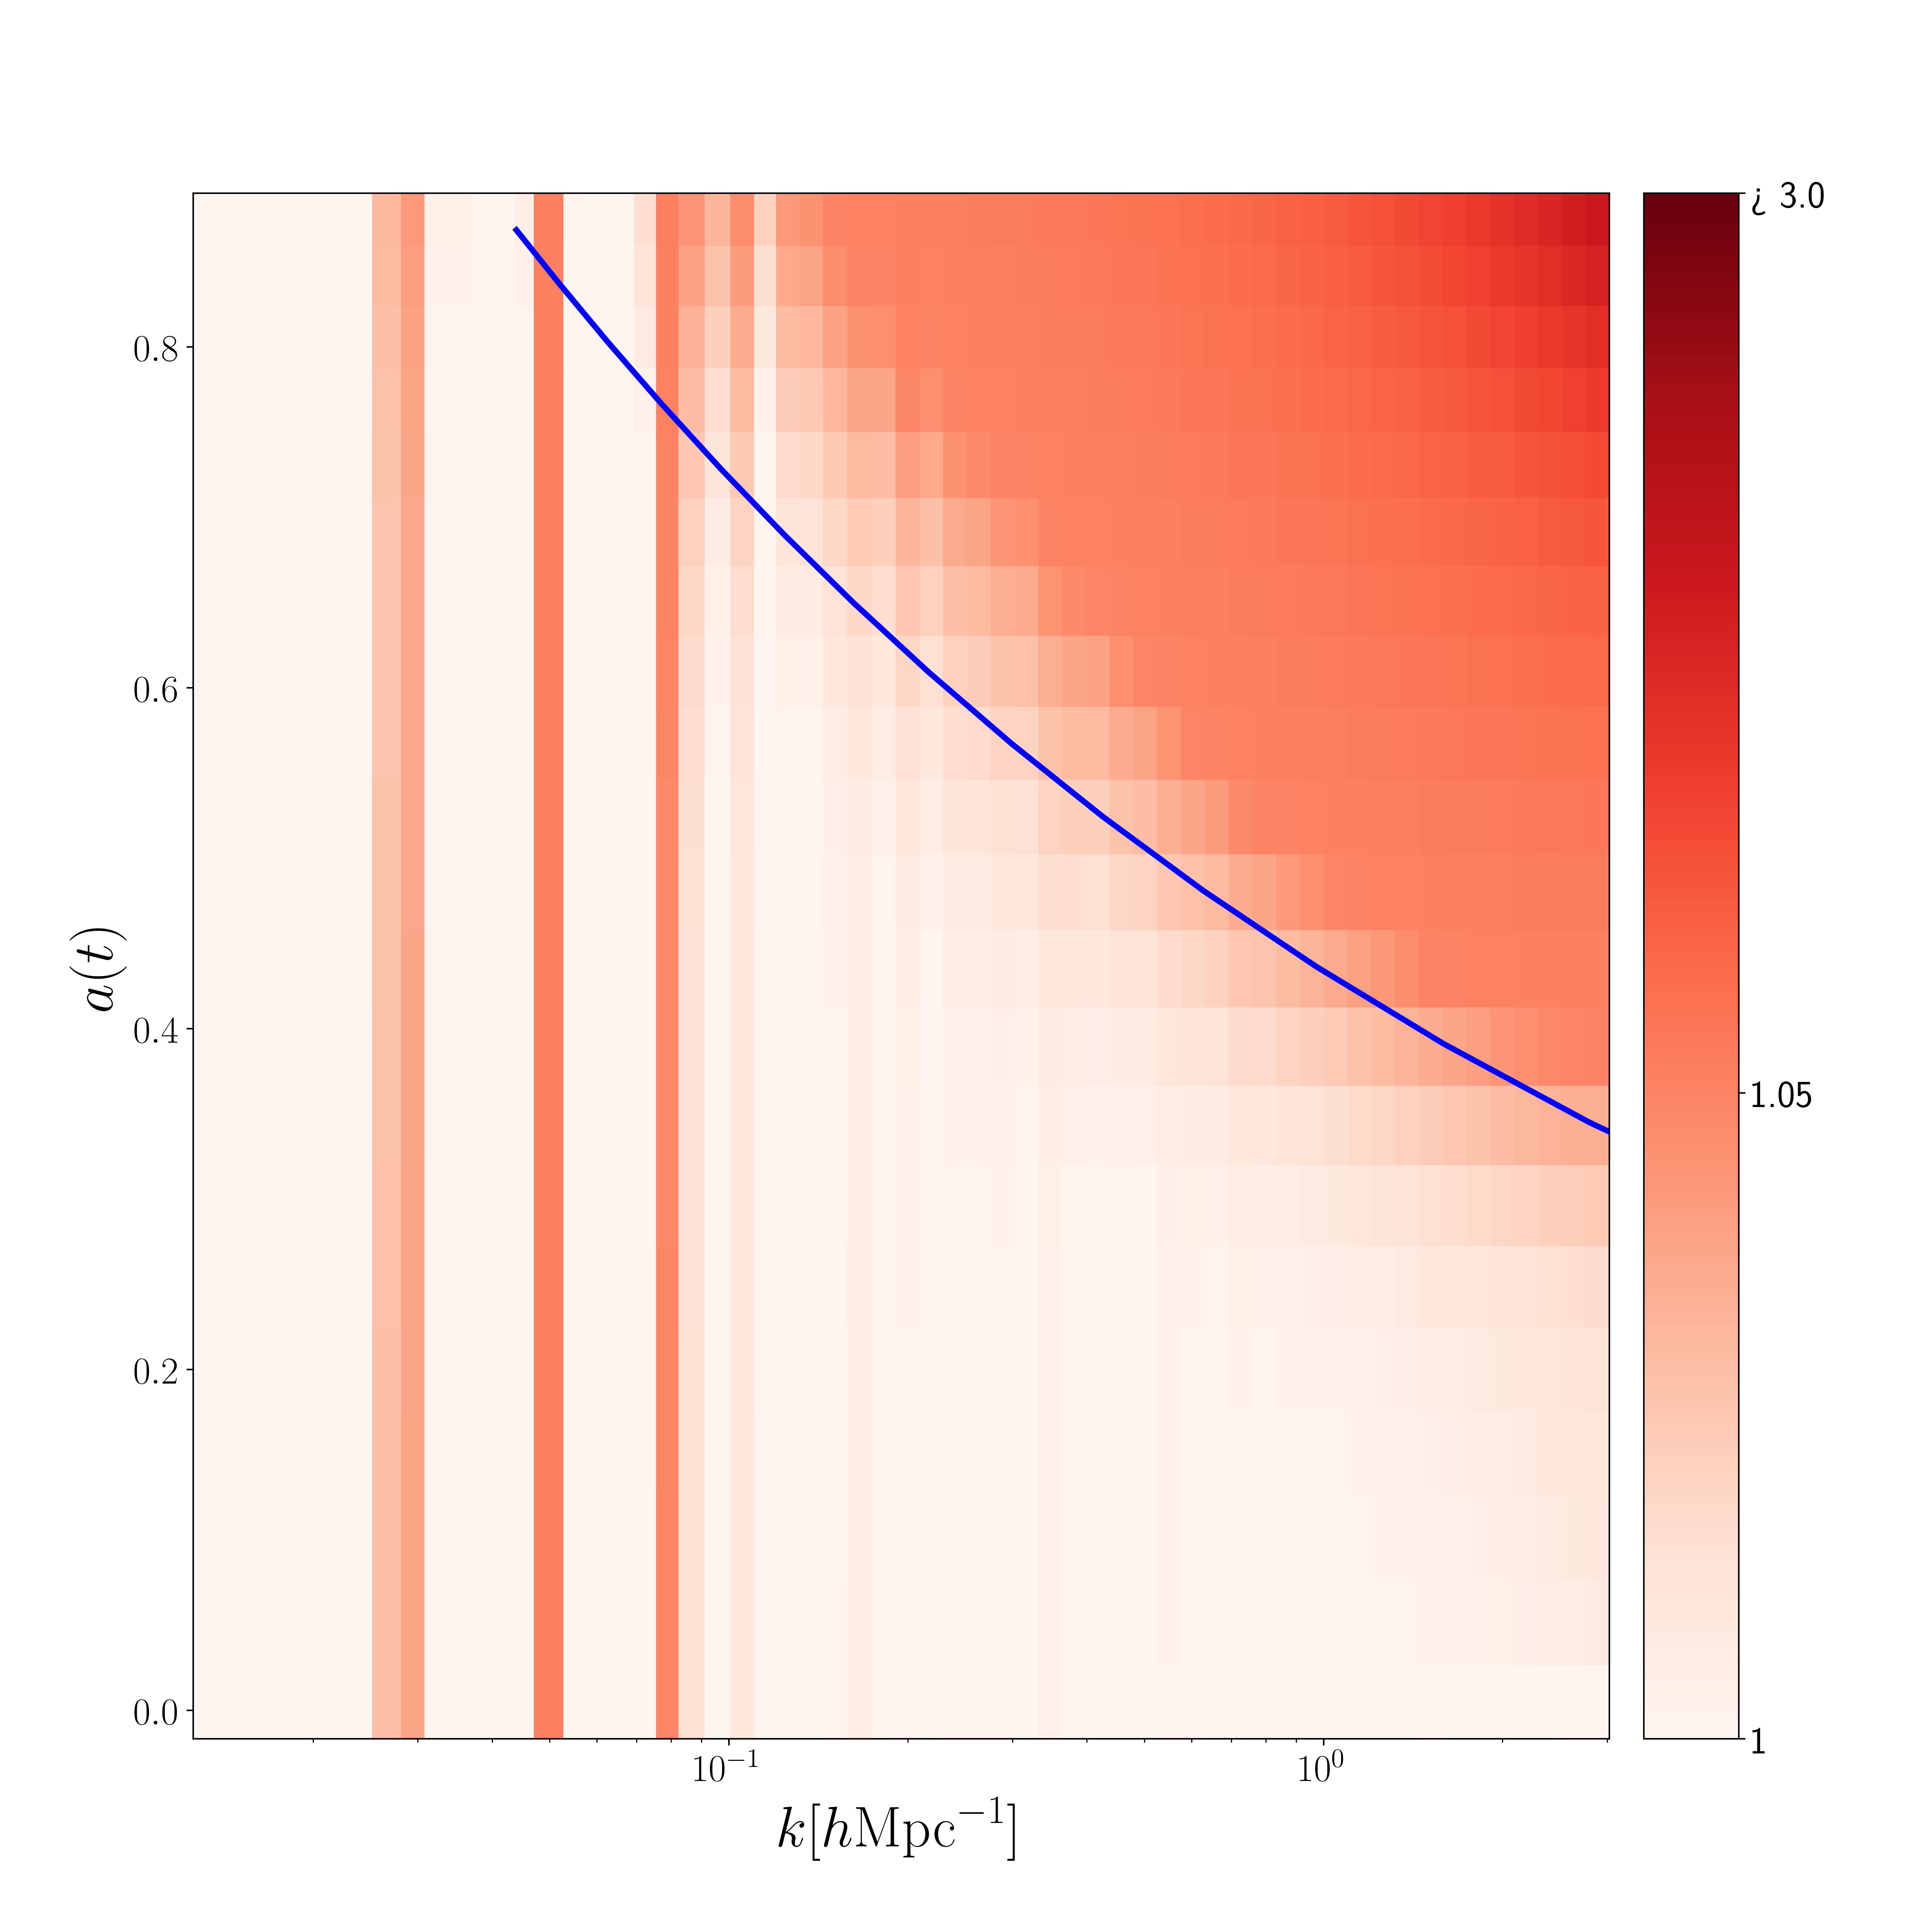
\includegraphics[width=0.7\linewidth]{simulations_approx/chi/chi_pwr_diff_map_512m_1p_1024M_500b_nl.png}
	\caption{Ratio of~the~FPA power spectrum in~chameleon gravity $(n=0.5,\ \Phiscr=10^{-5})$ to~the~simulation run with~standard gravity as a~function of~time. The~blue solid line is a~chameleon mass \eqref{eq:chi_m}.}
	\label{fig:chi_pwr_diff_map}
\end{figure}

\subsection{Correlation function}
In~\autoref{fig:chi_corr_func}, we display the~correlation function for~one particular case of~chameleon gravity -- $n=0.5,\ \Phiscr=10^{-5}$ at~$z=0.5$. In~\autoref{fig:chi_corr_peak}, we show the~effects of~different parameters of~chameleon gravity through the~BAO peak (amplitude, location, and~width). In~this plot, the~BAO peak characteristics are shown relative to~the~non-linear prediction (at~the~effective time) from the~emulator. Comparison is done both for~FPA (left) and~FFA (right). We see that chameleon generally leads to~a~higher amplitude of~the~peak, a~slight shift to~the~higher $r$, and~a~narrower width of~the~peak. All these effects are stronger for~FFA than for~FPA (as expected).

\begin{figure*}
\centering
	\begin{subfigure}{1.1\textwidth}
		\chileft
        \includegraphicscustomlegend{simulations_approx/chi/chi_corr_func_r2_z_z_eff}
	\end{subfigure}
	\begin{subfigure}{0.9\textwidth}
		\centering
		\includegraphicscustom{simulations_approx/chi/chi_corr_func_r2_z_z_eff}
	\end{subfigure}
	\begin{subfigure}{0.9\textwidth}
		\centering
		\includegraphicscustom{simulations_approx/chi/chi_ff_corr_func_r2_z_z_eff}
	\end{subfigure}
	\caption{Correlation function for~chameleon gravity $(n=0.5,\ \Phiscr=10^{-5})$ at~$z=0.5$. On~the~top are shown results using FPA whereas on~the~bottom using FFA.}
	\label{fig:chi_corr_func}
\end{figure*}

\begin{figure*}
\centering
	\begin{subfigure}{1.2\textwidth}
		\chileft
        \includegraphicscustomlegend{simulations_approx/chi/nl_fp_corr_peak_amp_z_eff}
	\end{subfigure}
	\begin{subfigure}{0.5\textwidth}
		\includegraphicscustom{simulations_approx/chi/nl_fp_corr_peak_amp_z_eff}
		\caption{Amplitude}
	\end{subfigure}
	\begin{subfigure}{0.5\textwidth}
		\includegraphicscustom{simulations_approx/chi/nl_ff_corr_peak_amp_z_eff}
		\caption{Amplitude}
	\end{subfigure}
	\begin{subfigure}{0.5\textwidth}
		\includegraphicscustom{simulations_approx/chi/nl_fp_corr_peak_loc_z_eff}
		\caption{Location}
	\end{subfigure}
	\begin{subfigure}{0.5\textwidth}
		\includegraphicscustom{simulations_approx/chi/nl_ff_corr_peak_loc_z_eff}
		\caption{Location}
	\end{subfigure}
	\begin{subfigure}{0.5\textwidth}
		\includegraphicscustom{simulations_approx/chi/nl_fp_corr_peak_width_z_eff}
		\caption{Width}
	\end{subfigure}
	\begin{subfigure}{0.5\textwidth}
		\includegraphicscustom{simulations_approx/chi/nl_ff_corr_peak_width_z_eff}
		\caption{Width}
	\end{subfigure}
	\caption{Location, amplitude and~width of~the~BAO peak as a~function of~the~redshift for~different values of~chameleon parameters. On~the~left, the~characteristics are shown for~simulations using FPA, while on~the~right, for~simulations using FFA.}
	\label{fig:chi_corr_peak}
\end{figure*}

\subsection{Halo mass function}
In~\autoref{fig:chi_diff_hmf} we compared the~(relative) halo mass function for~different parameters of~chameleon gravity. We use the~halo mass function relative to~the~non-linear prediction (at~the~effective time) from the~emulator. Comparison is done both for~FPA (top) and~FFA (bottom). We see that for~FPA in~the~mass range $(10^{12}-10^{14}M_\odot)$ all the~simulations give very similar results and~differ more outside this range. FFA shows much greater differences between individual parameters, as we have already seen in~the~correlation function. For~both approximations, we see that the~higher the~screening potential $\Phiscr$ the~more power on~small scales and~therefore more massive halos. For~distinguishing between different chameleon parameters we should, therefore, use the~most massive halos $(M\gtrsim10^{14}M_\odot)$.
\begin{figure*}
	\centering
	\chileft
	\begin{subfigure}{1.2\textwidth}
		\includegraphicscustomlegend{simulations_approx/chi/hmf_z0.5_b2000_M512_chi_hmf_z_z_eff}
	\end{subfigure}
	\begin{subfigure}{1.0\textwidth}
		\centering
		\includegraphicscustom{simulations_approx/chi/hmf_z0.5_b2000_M512_chi_hmf_z_z_eff}
	\end{subfigure}
	\begin{subfigure}{1.0\textwidth}
		\centering
		\includegraphicscustom{simulations_approx/chi/hmf_z0.5_b2000_M512_chi_ff_hmf_z_z_eff}
	\end{subfigure}
	\caption{Halo mass function (relative) for~non-linear chameleon gravity with~different chameleon parameters. On~the~top are shown results using FPA whereas on~the~bottom using FFA.}
	\label{fig:chi_diff_hmf}
\end{figure*} 
\section{Discussion}
\label{sec:disc}
In this chapter, we studied different approximation schemes and tested their usefulness as fast alternatives to full \nbodysim s. The results for ZA and TZA are as expected. Both of these approximations may be used to make very fast predictions (no need for trajectory integration). Speed (and other computation resources) is the main advantage of ZA and TZA but at the cost of reduced accuracy. We saw that they predict very good results on large scales $(k<10^{-2}~\hMpc)$ but structures on smaller scales are smeared out due to the line-crossing. TZA proved to work better on these smaller scales but at the cost of loss of sub-structures.

FFA and FPA have better results on our scales of interest -- they predict better location and width of the BAO peak for redshifts $z\gtrsim0.5$ than ZA or TZA. Their main disadvantage compared to the ZA or TZA is speed because we need to integrate the whole trajectory through the frozen field (velocity or gravitational potential). Although they are slower than ZA and TZA, they are still much faster than full \nbodysim s. Because we do not need to compute the short range force and the density field at each time-step and the surrounding field remains (almost) constant, we can use much larger time-steps than in full \nbodysim s. Because particles do not \textit{see} each other, we can integrate their paths independently -- from the starting redshift to the final one with adaptive time-step which can further improve the overall speed and accuracy.

In FFA and FPA, structures grow more slowly than in the case of the linear theory. This feature of the approximations can be fixed through mapping of the simulation time and real time. With this fix, structures grow on all scales (there is no smearing on small scales as in the case of ZA/TZA) and there are even non-linear features in the power spectrum. We also showed that this slower growth is not due to the insufficient number of time-steps as may be the case for standard PM simulations. Summary of the achieved accuracy is shown in \autoref{tab:err}.

All approximations can predict the BAO peak location to a 1\% accuracy at $z=0.5$, comparing to a non-linear theory. However, ZA and TZA predict the smoothing of the peak stronger than non-linear evolution \parencite[see, e.g.,][]{2007ApJ...664..660E, 2014JCAP...02..042S} whereas FFA and FPA weaker. All approximations predict lower amplitude and narrower width of the peak than linear theory (smoothing). ZA and TZA predict a wider peak, while FPA and FFA a narrower one, as compared to the $N$-body prediction. Compared to the amplitude of the BAO peak of the $N$-body prediction ZA and TZA give the best results for low $z$. However, for higher redshifts $z>1$, FFA and FPA give better amplitude, location and width.
\begin{table}
\centering
\begin{tabular}{lccccc}
	\hline \hline
	 & $P_1(k)$ & $P_2(k)$ & amp & loc & width \\ 
	\hline
	FF & $1.3\%$ & $8.2\%$ & $11.2\%$ & $0.4\%$ & $5.2\%$ \\
	FP & $2.1\%$ & $8.2\%$ & $8.7\%$ & $0.3\%$ & $2.9\%$ \\
	TZA & $11.3\%$ & $33.0\%$ & $5.2\%$ & $0.9\%$ & $13.4\%$ \\
	ZA & $6.4\%$ & $17.2\%$ & $0.2\%$ & $0.5\%$ & $8.4\%$ \\
	\hline \hline
\end{tabular}
 \caption
{Errors of different approximation schemes at the redshift $z=0.5$. $P_1(k)$ corresponds to an error at scale $k = 0.1~\hMpc$ and $P_2(k)$ at scale $k = 0.2~\hMpc$. Amp, loc and width are errors of the BAO peak.}
\label{tab:err}
\end{table}

The broadening and shift of the acoustic peak due to the non-linear evolution of structures can be reduced by reconstruction techniques \parencite{2007ApJ...664..675E}. A widely used technique is based on ZA, as described in \textcite{10.1111/j.1365-2966.2012.21888.x}. As FFA and FPA are closer to the non-linear evolution than ZA or TZA, they could potentially be used for similar purposes.

Different approximation methods -- Lagrangian perturbation theory (LPT) up to third order (\cite{10.1093/mnras/264.2.375}), Truncated LPT (\cite{1993MNRAS.260..765C}), Augumented LPT (\cite{10.1093/mnrasl/slt101}), MUSCLE (\cite{10.1093/mnrasl/slv141}) and COLA -- have been tested in \textcite{2017JCAP...07..050M}, see \autoref{fig:app_compare}. Our results for ZA and TZA match theirs (on the basis of matter power spectrum accuracy at the scale $k=0.1~\Mpch$ and $k=0.2~\Mpch$, see \autoref{tab:err}). Our results for FFA and FPA show that they do better than 2LPT ($\sim5\%$ error of $P(k)$ at $k=0.1~\Mpch$ at $z=0.5$) and T2LPT $(\sim10\%)$, while having a similar accuracy as compared to 3LPT $(\sim1\%)$, A2LPT $(\sim1\%)$, A3LPT $(\sim2\%)$ and MUSCLE 2LPT $(\sim1\%)$. As expected, the particle-mesh code COLA gives the best results, especially at later time $(z=0)$.

\begin{figure}[!htb]
  \centering
  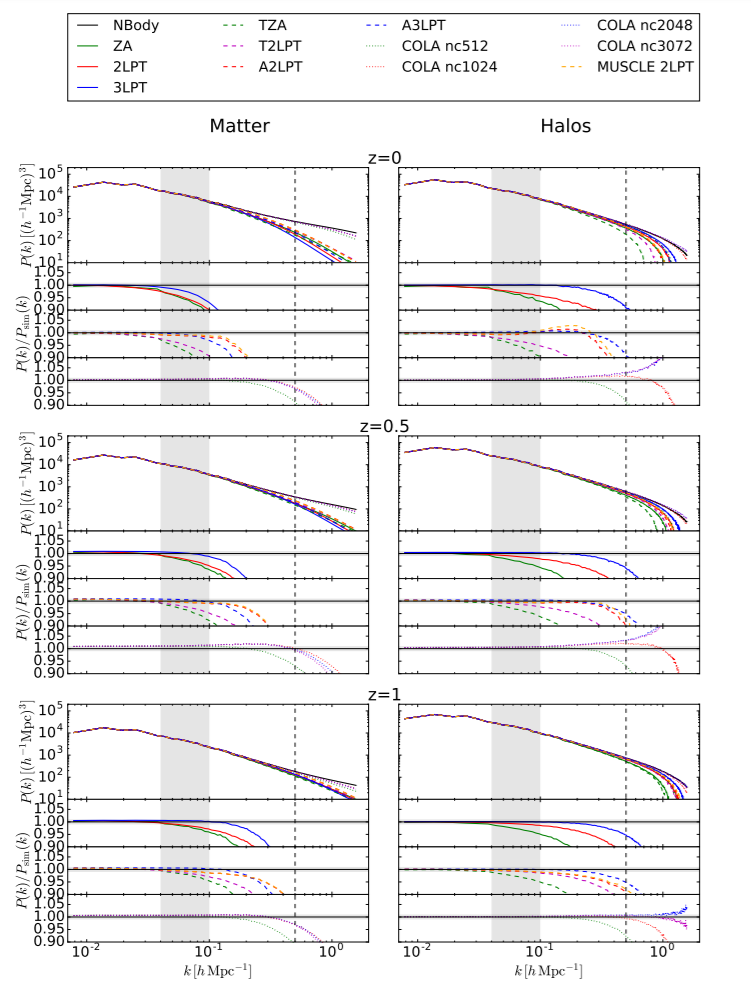
\includegraphics[width=0.9\textwidth]{cosmo_evol/app_compare.png}
  \caption{Power spectrum at~$z = 0,\ 0.5$, and~$1$ (top, middle, and~bottom panels, respectively) in~real space and~ratio with~the~\nbody’s one for~the~matter field (left panels) and~the~halo catalogs (right panels). The~vertical dashed line locates the~$k = 0.5\hMpc$ where the~one-halo term becomes significant. The~vertical shaded area locates the~region of~the~BAO peak, while the~horizontal one locates the~1\% accuracy region.  \textit{Note:} Reprinted from \textcite{2017JCAP...07..050M}.}
  \label{fig:app_compare}
\end{figure}
When we applied the FPA to chameleon gravity we saw that the spatial resolution of simulations has a great impact on the resulting power spectra (on small scales). In our code, we used a fixed-size mesh. However, when entering the screening regime where high resolution is key, the use of an adaptive mesh would be a better approach. Note that the limitations of the approximations on small scales must be taken into account. This limits the highest possible resolution to $k\sim1~\Mpch$ that is still reasonable to use.

For studying large scales $(k\lesssim0.1~\hMpc)$ both pseudo-linear and non-linear prediction had very similar results. We saw that the pseudo-linear solution to chameleon equations generally predicts a greater effect of the fifth force than the non-linear solution on smaller scales. On small scales $(k\gtrsim1~\hMpc)$ the difference between the pseudo-linear and non-linear solutions became more apparent in the screening regime. The scale when this transition happens tells us where the results of linear prediction are still sufficient and when the linear prediction breaks down.

The overall success of FFA and FPA when predicting the movement of particles reveals that linear predictions of potentials can lead to good results. This could also be applied to a non-linear solver for the chameleon equations where the linear prediction is relatively close to the non-linear one on large scales and at early times. For now, at each time-step we recomputed the chameleon field. But in principle we can compute the chameleon field only once in a while -- depending on the background chameleon values and the number of regions in the screened regime -- and evolve the chameleon field according to the linear theory in between.

To sum up, we showed that simple methods like FFA and FPA, which are very easy to implement even for modified theories of gravity, can predict results at BAO scales that are comparable with significantly more complex methods such as second-order Lagrangian perturbation theory. This makes their further study worthwhile, including implementations for other modified gravity models.\clearpage{}
\clearpage{}\chapter{Outlook}
\label{chpt:outlook}
In~the~thesis, we explored different ways to~study modified gravities. The~work was focused on~quasi-linear regimes as the~full non-linear behavior of~modified gravities is hard to~study due to~its numerical difficulties. We showed what behavior one can expect on~scales ranging from stars to~that of~superclusters. The~implemented methods were tested on~the~example of~the~chameleon gravity and~showed interesting results. These prepared techniques can now be used to~explore other modified gravities.

In~\autoref{chpt:de_mg} we studied the~properties of~the~chameleon gravity in~spherical systems -- stars and~in~NFW halos both on~scales of~galaxies and~clusters of~galaxies. Although the~results showed that the~Hu-Sawicki \fR\ theory is screened in~this system, other modifications of~gravity do not have to~be and~it is worth checking. Our code and~implemented techniques can be used with~slight modifications for~studies of~a~broader class of~theories. Implementing other models of~\fR\ gravity exhibiting chameleon mechanism should be fairly straightforward and~therefore we would like to~explore this type of~modification in~a~similar way as we did for~the~Hu-Sawicki model.

We would like to~study the~generic \fR\ models with~negative and~positive powers of~curvature of~\textcite{2003PhRvD..68l3512N} which can in~principle unify the~inflation and~cosmic acceleration. The~model is given by
\eq{
    f(R)=R-\frac{a}{(R-\Lambda_1)^n}+b(R-\Lambda_2)^m\,.
}
Another class of~models we would like to~explore was proposed by \textcite{2007JETPL..86..157S}. This class of~modifications is given by
\eq{
    f(R)=R+\lambda R_0\left[\left(1+\frac{R^2}{R_0^2}\right)^{-n}-1\right]\,.
}
All of~these models can be studied in~dense objects surrounded by a~vacuum (or decreasing density) such as stars and~halos as we did in~this work. Another approach, which can be tested in~laboratory conditions on~Earth, is quite the~opposite. We can study the~behavior of~the~chameleon in~a~vacuum chamber surrounded by a~dense environment. This could be implemented easily in~our code and~is therefore worth studying. However, we showed that the~effective screening potential is very low on~scales of~galaxies and~can range from $10^{-10}$ up to~completely screened values of~the~order $10^{-40}$, depending on~the~parameter $n$. Fow a~wide range $(0.1 < n < 1)$ we do not expect this will lead to~measurable results but for~the~low values $(n < 0.1)$ it could lead to~some measurable effects.

The~main field for~studying modified gravities remains on~cosmological scales where it mimics the~cosmological constant. In~the~work, we dealt with~approximations which can greatly help to~study quasi-linear regimes. Although the~non-linear results for~used approximation schemes do not look very promising compared to~simple particle-mesh codes such as \code{COLA} they proved that linear approximation can be used successfully and~we can still obtain results in~mildly non-linear regimes. This can be used for~studies of~modified gravity where solving the~full non-linear equations is computationally very demanding and~probing the~huge space of~different modifications almost impossible. We showed that linear approximation of~chameleon equations can still lead to~observable non-linear results.

This approach we want to~pursue further, i.e. to~use particle-mesh codes such as \code{COLA}, \code{HACC}, or \code{GADGET} without demanding short-range interactions and~implement modified equations for~theories such as chameleon. To~speed up the~execution time we would use the~linear predictions for~these theories which we saw can still lead to~non-linear results. This will further push the~scales where we can study the~chameleon behavior down and~it will increase current precision at~the~BAO scale.

The~next step we can make in~studying the~non-linear regime with~modified gravities is to~use \nbody\ code with~short-range forces, use the~linear predictions for~chameleon gravity to~avoid the~lengthy computation of~the~chameleon field and~therefore obtain a~good approximation of~the~background value of~the~field. To~solve the~equations on~small scales quickly we would use the~introduced technique for~spherical systems. As the~halo finders are a~standard part of~the~simulations, obtaining some approximate density profile of~forming halos would not be too expensive. Consequent solving of~the~one-dimensional chameleon non-linear equations does not pose any substantial demands on~computing time.\clearpage{}
\clearpage{}\chapter*{Conclusion}
\addcontentsline{toc}{chapter}{Conclusion}
The~thesis was dealing with~the~topic of~modified gravity and~how we can discover its resulting deviations from general relativity. In~\autoref{chpt:cosmo_evol} we summarized linear equations for~the~evolution of~the~Universe. We described how we can use the~evolution process to~studies of~cosmological parameters of~the~Universe. We described basic cosmological observables and~their usefulness when distinguishing between different cosmologies.

\hyperref[chpt:de_mg]{Chapter 2} was focused on~modifications of~the~general relativity. We described successes and~failures of~the~standard cosmological model and~presented main issues with~the~cosmological constant. We described how we can modify the~theory of~gravity and~focused on~one of~the~most studied extensions -- the~\fR\ gravity. We studied the~Hu-Sawicki \fR\ theory from a~different angle of~view than most authors -- as the~chameleon gravity in~the~Einstein frame. We studied the~chameleon behavior numerically and~we checked the~linear predictions with~our numerical solutions. We studied the~chameleon behavior in~spherical systems (stars, galaxies, clusters) and~concluded that the~chameleon mechanism hides the~fifth force on~scales smaller than superclusters for~the~Hu-Sawicki model and~that the~chameleon needs to~be studied on~large cosmological scales through \nbodysim s. Our original method of~solving modified gravity in~spherical systems represents an~important contribution because it can be applied to~other models than Hu-Sawicki \fR. With~these methods we can check the~behavior of~other theories in~spherical systems and~also check their behavior in~laboratory conditions on~the~Earth.

In~\autoref{chpt:cosmo_sim} we described general techniques when dealing with~cosmological \nbodysim s and~how we implemented them in~our own code for~\nbodysim s -- with~both standard and~modified gravity. We described our own contribution to~the~\code{CCL} code and~how the~\code{CCL} can help scientists worldwide to~speed up their work on~cosmology.

In~\autoref{chpt:app_schemes} we introduced different approximations that can be used to~study the~Universe quickly and~intuitively. Most of~the~previous studies focused on the~Einstein--de Sitter Universe whereas in~this work we generalized the~equations to~the~\LCDM\ cosmology. We described how we implemented these approximations in~studies of~modified gravity which has not been done before and~is one of~the~original result of~this work.

Key results of~the~thesis are presented in~\autoref{chpt:app_sims}. We described original results of~our cosmological \nbodysim s using approximate schemes. We focused on~aspects that have drawn less attention in~the~past -- slower growth of~structure formation (modified growth function), study of~the~correlation function, predictions of~the~shape of~the~peak of~baryonic acoustic oscillations in~real space and~the~ability to~predict certain non-linear features of~full \nbodysim s. We showed that these approximations can be used to~study scales around the~baryon acoustic oscillation scale, $k\sim 0.1~h\text{Mpc}^{-1}$ but not much further. We also tested these methods on~the~chameleon gravity and~showed what probes are suited the~best for~distinguishing between different parameters of~the~chameleon gravity. Unlike matter power spectra and~baryonic acoustic oscillation, the~halo mass function does not seem to~be a~good way to~study the~chameleon gravity. In~\autoref{chpt:outlook} we then discussed other possible applications of~approximate methods described in~this work and~we outlined further course of~our studies.

In~\autoref{chpt:cosmo_surveys} we reviewed the~present-day and~future experiments designed to~study our Universe. We showed what constraints on~our Universe have already been observed and~what accuracy of~future experiments we can expect.

\subsubsection{Author's publications}
\begin{refsection}[bibliography/my_work.bib]
In~the~\hyperref[chpt:list_publish]{List of~publications} all author's publications are listed (in~alphabetical order by the~authors' last names). The~list includes the~author's previous work in~the~Cherenkov Telescope Array collaboration \parencite{2016arXiv161005151C,2017arXiv170903483A,2017ApJ...840...74A,2019scta.book.....C}. While working on~the~CTA, the~author's main interest were the~atmospheric simulations of~cosmic showers \parencite{2017EPJWC.14401014V,}. The~purpose of~these simulations is to~improve the~calibration of~the~atmospheric properties as well as a~calibration of~the~detector response. One of~the~main contributions to~the~systematic uncertainties of~the~CTA measurements stems from the~uncertainty on~the~atmospheric density profile, of~molecules and~aerosols, which these simulations help to~reduce.

The~author's work inside the~Dark Energy Science Collaboration (DESC) focused mainly on~improving the~Core Cosmology Library \parencite[\code{CCL},][]{2019ascl.soft01003C,2019ApJS..242....2C}. Initially, the~author helped to~create a~documentation of~the~library, wrote many examples of~usage of~the~\code{CCL}, and~presented with~other authors the~\code{CCL} and~its capabilities at~several sessions to~new users. The~author also helped to~improve several automatization processes regarding the~releasing of~the~library and~helped to~improve its compatibility across different operating systems and~environments.

The~author's main work, \textit{Fast approximate methods for~modified gravity cosmological simulations} \parencite[published in~Monthly Notices of~the~Royal Astronomical Society,][]{2020MNRAS.493.2085V}, summarizes results regarding the~cosmological \nbodysim s described in~this work (\autoref{chpt:cosmo_sim} -- \autoref{chpt:app_sims}). It is the~result of~several-year research regarding the~cosmological simulations. During this time, the~author wrote his own code for~cosmological simulations, implemented methods for~solving highly non-linear equations, and~developed complex pipelines for~processing and~analyzing data of~these simulations.
\end{refsection}
\clearpage{}


\cleardoublepage
\phantomsection
\renewcommand{\bibname}{Bibliography}
\addcontentsline{toc}{chapter}{\bibname}
\begingroup
\sloppy
\printbibliography[title={\bibname}]
\endgroup



\cleardoublepage
\phantomsection
\renewcommand{\bibname}{List of~publications}
\addcontentsline{toc}{chapter}{\bibname}
\label{chpt:list_publish}
\begin{refsection}[bibliography/my_work.bib]
\nocite{*}
\begingroup
\sloppy
\printbibliography[title={\bibname}]
\endgroup
\end{refsection}



\openright
\end{document}
